\documentclass{tufte-book} 
% This configures what chapters are rendered and what aren't
\newif\ifSpIntro
\newif\ifSpPython
\newif\ifSpComplex
\newif\ifSpSigSys
\newif\ifSpElSig
\newif\ifSpSin
\newif\ifSpFourierSer
\newif\ifSpFourierTra
\newif\ifSpDT
\newif\ifSpLTI
\newif\ifSpFResp
\newif\ifSpDTFT
\newif\ifSpFilters
\newif\ifSpUncertainty
\newif\ifSpDFT
\newif\ifSpSpectAn
\newif\ifSpFiltering
\newif\ifSpZFIR
\newif\ifSpZIIR
\newif\ifSpdB
\newif\ifSpProgA
\newif\ifSpProgB
\newif\ifSpProgC
\newif\ifSpSyllabus

\newif\ifSpExerciseSol


% Comment out to disable chapter/section
% look in signal_processing.tex to see what is affected by these
% if statements

\if 0
\SpExerciseSolfalse        % turn exercise solutions on/off
\SpSyllabustrue        %syllabus
\SpIntrotrue        %ch01
\SpPythonfalse       %ch02
\SpComplexfalse      %ch03
\SpSigSysfalse       %ch04
\SpElSigfalse        %ch05
\SpSinfalse          %ch06
\SpdBfalse           
\SpFourierSerfalse   %ch07
\SpFourierTrafalse   %ch08
\SpDTfalse           %ch09
\SpLTIfalse          %ch10
\SpFRespfalse        %ch11
\SpDTFTfalse         %ch12
\SpFiltersfalse      %ch13
\SpUncertaintyfalse  %ch14
\SpDFTfalse          %ch15
\SpSpectAnfalse      %ch16
\SpFilteringfalse    %ch17
\SpZFIRfalse         %ch18
\SpZIIRfalse         %ch19

% turn off programming assignments
\SpProgAfalse        %p1
\SpProgBfalse        %p2
\SpProgCfalse        %p3
\fi

\SpExerciseSoltrue        % turn exercise solutions on/off
\SpSyllabustrue        %syllabus
\SpIntrotrue        %ch01
\SpPythontrue       %ch02
\SpComplextrue      %ch03
\SpSigSystrue       %ch04
\SpElSigtrue        %ch05
\SpSintrue          %ch06
\SpFourierSertrue   %ch07
\SpFourierTratrue   %ch08
\SpDTtrue           %ch09
\SpLTItrue          %ch10
\SpFResptrue        %ch11
\SpDTFTtrue         %ch12
\SpFilterstrue      %ch13
\SpUncertaintytrue  %ch14
\SpDFTtrue          %ch15
\SpSpectAntrue      %ch16
\SpFilteringtrue    %ch17
\SpZFIRtrue         %ch18
\SpZIIRtrue         %ch19

% turn off programming assignments
\SpProgAtrue        %p1
\SpProgBtrue        %p2
\SpProgCtrue        %p3

%=======
%\SpProgCtrue        %p3
%>>>>>>> e63d22f87b61765fe8f4e43f9ba97a3923d3e76e
 
\usepackage[english]{babel}
\usepackage[utf8x]{inputenc}
\usepackage[T1]{fontenc}
%% Sets page size and margins
%\usepackage[a4paper,top=3cm,bottom=2cm,left=3cm,right=3cm,marginparwidth=1.75cm]{geometry}

%% Useful packages
\usepackage{amsmath,amssymb,amsthm}
\usepackage{physics}
\usepackage{mathtools}
\usepackage{tikz}
\usepackage{pgfplots}
\usepackage{graphicx}
\usepackage{xcolor}
\usepackage{tabularx}

\usepackage[colorinlistoftodos]{todonotes}

%\usetikzlibrary{backgrounds,calc}

\usetikzlibrary{shapes,arrows,backgrounds,calc}
\usepackage{color}
\usepackage{listings}
\usepackage{bm}
\usepackage{microtype} % Improves character and word spacing
\usepackage{lipsum} % Inserts dummy text
\usepackage{booktabs} % Better horizontal rules in tables
\usepackage{graphicx} % Needed to insert images into the document
\usepackage{tabularx}
\usepackage{cancel}
\definecolor{codegreen}{rgb}{0,0.6,0}
\definecolor{codegray}{rgb}{0.5,0.5,0.5}
\definecolor{codepurple}{rgb}{0.58,0,0.82}
%\definecolor{backcolour}{rgb}{0.95,0.95,0.92}
%\definecolor{backcolour}{rgb}{0.5,0.5,0.5}
%\definecolor{backcolour}{rgb}{1.0,0.937,0.859}
\definecolor{backcolour}{rgb}{1.0,1.0,1.0}
\definecolor{skyblue1}{rgb}{0.447,0.624,0.812}
\definecolor{scarletred1}{rgb}{0.937,0.561,0.561}
\definecolor{juhagray}{rgb}{0.75,0.75,0.75}
%\definecolor{backcolour}{rgb}{1.0,1.0,1.0}
 
\lstdefinestyle{mystyle}{
    backgroundcolor=\color{backcolour},   
    commentstyle=\color{codegreen},
    keywordstyle=\color{magenta},
    numberstyle=\tiny\color{codegray}, 
    stringstyle=\color{codepurple},
    basicstyle=\footnotesize,
    breakatwhitespace=false,
    frame=shadowbox,
    rulesepcolor=\color{juhagray},
    breaklines=true,                 
    captionpos=b,                    
    keepspaces=true,                 
    numbers=none,                    
    numbersep=5pt,                  
    showspaces=false,                
    showstringspaces=false,
    showtabs=false,                  
    tabsize=2
}
 
\lstset{style=mystyle}

\usepackage[american,siunitx]{circuitikz}
\usetikzlibrary{arrows,calc,positioning}


\newcommand{\Hee}{\mathcal{H}(e^{i\hat{\omega}})}
\newcommand{\Hez}{\mathcal{H}(z)}
\newcommand{\Hew}{\mathcal{H}(\omega)} 
\newcommand{\Hec}{\mathcal{H}^*\left(e^{i\hat{\omega}}\right)} 
\newcommand{\Hem}{\mathcal{H}\left(e^{-i\hat{\omega}}\right)}
%\newcommand{\He}{\mathcal{H}\left(e^{i\hat{\omega}}\right)}

\newcommand{\He}{\mathcal{H}\left(\hat{\omega}\right)}
\newcommand{\Xe}{X\left(e^{i\hat{\omega}}\right)}
\newcommand{\Xec}{X^*\left(e^{i\hat{\omega}}\right)}
%\newcommand{\Hec}{\mathcal{H}^*\left(e^{i\hat{\omega}}\right)} 
%\newcommand{\Hem}{\mathcal{H}\left(e^{-i\hat{\omega}}\right)} 
\newcommand{\Xem}{X\left(e^{-i\hat{\omega}}\right)} 

\newcommand{\mixer}[1] 
{  % #1 = name , 
\draw[thick] (#1) circle (12pt);
\draw[rotate=45,line width=0.5pt]   (#1)  +(0,-12pt) -- +(0,12pt);
\draw[rotate=-45,line width=0.5pt]  (#1)  +(0,-12pt) -- +(0,12pt);
}
\newcommand{\BPF}[2] 
{  % #1 = name , #2 = rotation angle
\begin{scope}[transform shape,rotate=#2]
\draw[thick] (#1)node[](a){} +(-12pt,-12pt) rectangle +(12pt,12pt);
\draw (a) +(-8pt,0) to[bend left] +(0,0) edge[bend right] +(8pt,0);
\draw ([yshift=5pt]a) +(-8pt,0) to[bend left] +(0,0) to[bend right] +(8pt,0);
\draw ([yshift=-5pt]a) +(-8pt,0) to[bend left] +(0,0) edge[bend right] +(8pt,0);
\draw[rotate=20] ([yshift=5pt]a) +(-4pt,0) -- +(7pt,0);
\draw[rotate=20] ([yshift=-5pt]a) +(-7pt,0) -- +(4pt,0);
\end{scope}
}
\newcommand{\LPF}[2] 
{  % #1 = name , #2 = rotation angle
\begin{scope}[transform shape,rotate=#2]
\draw[thick] (#1)node[](a) {\footnotesize{$\mathcal{H}(\omega)$}} +(-12pt,-12pt) rectangle +(12pt,12pt);
\end{scope}
}

\newcommand{\hangp}[1]{\makebox[0pt][r]{(}#1\makebox[0pt][l]{)}} % New command to create parentheses around text in tables which take up no horizontal space - this improves column spacing
\newcommand{\hangstar}{\makebox[0pt][l]{*}} % New command to create asterisks in tables which take up no horizontal space - this improves column spacing

\tikzset{ar/.style={-latex,shorten >=-1pt, shorten <=-1pt}}
\usetikzlibrary{shapes,arrows}


\hypersetup{colorlinks} % Comment this line if you don't wish to have colored links


\setkeys{Gin}{width=\linewidth,totalheight=\textheight,keepaspectratio} % Improves figure scaling

\usepackage{fancyvrb} % Allows customization of verbatim environments
\fvset{fontsize=\normalsize} % The font size of all verbatim text can be changed here


\usepackage{xspace} % Used for printing a trailing space better than using a tilde (~) using the \xspace command

\newcommand{\monthyear}{\ifcase\month\or January\or February\or March\or April\or May\or June\or July\or August\or September\or October\or November\or December\fi\space\number\year} % A command to print the current month and year

\newcommand{\openepigraph}[2]{ % This block sets up a command for printing an epigraph with 2 arguments - the quote and the author
\begin{fullwidth}
\sffamily\large
\begin{doublespace}
\noindent\allcaps{#1}\\ % The quote
\noindent\allcaps{#2} % The author
\end{doublespace}
\end{fullwidth}
}
\usetikzlibrary{shapes,snakes}

\newcommand\Hiw{\mathcal{H}(\omega)}

\tikzset{%
    dimen/.style={|-|,>=latex,thin,every rectangle node/.style={fill=white,midway,font=\sffamily}},
}

\pgfplotsset{
    dirac/.style={
        mark=triangle*,
        mark options={scale=2},
        ycomb,
        scatter,
        visualization depends on={y/abs(y)-1 \as \sign},
        scatter/@pre marker code/.code={\scope[rotate=90*\sign,yshift=-2pt]}
    }
}

\tikzstyle{int}=[draw, minimum size=2em]
\tikzstyle{init} = [pin edge={to-,thin,black}]

 
\newcommand{\spop}[1][\cdot]{\mathcal{T}\left\{#1\right\}}
\newcommand{\spopb}{\mathcal{T}}

\newcommand{\blankpage}{\newpage\hbox{}\thispagestyle{empty}\newpage} % Command to insert a blank page

\usepackage{imakeidx} % Used to generate the index
\usepackage{hyperref}
\makeindex % Generate the index which is printed at the end of the document

\setcounter{secnumdepth}{0} %numbers chapters

%----------------------------------------------------------------------------------------
%	BOOK META-INFORMATION
%----------------------------------------------------------------------------------------
\author{Juha Vierinen} % Author
\publisher{University of Troms\o{}} % Publisher

%----------------------------------------------------------------------------------------


\newsavebox{\titleimage}
\savebox{\titleimage}{
\centering{
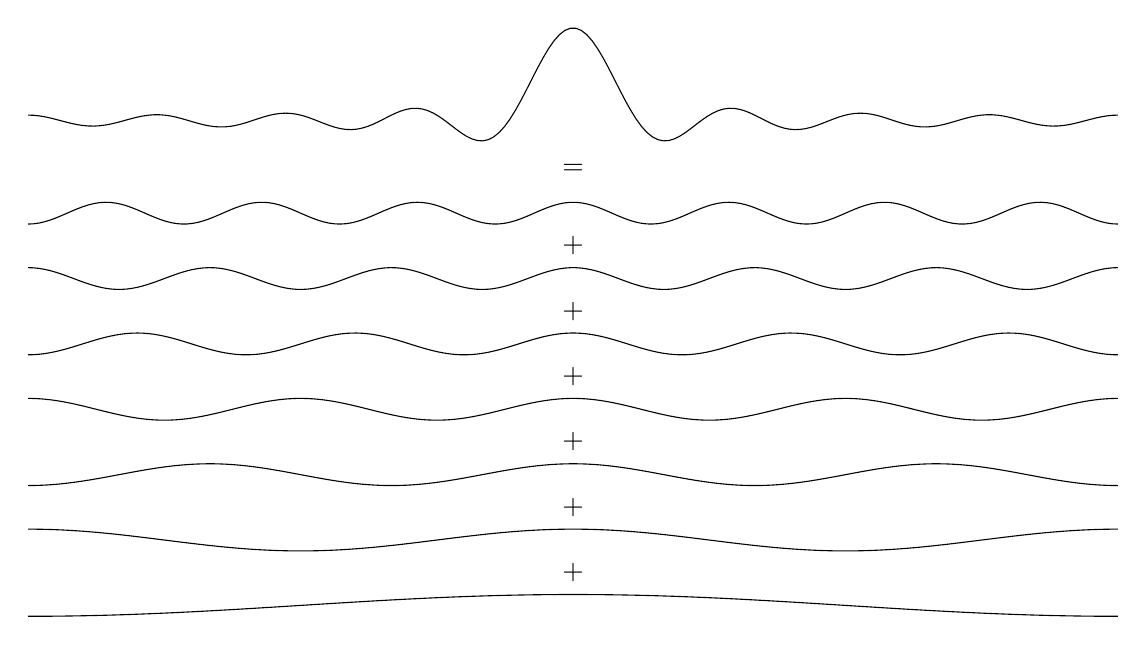
\begin{tikzpicture}
% \begin{pgfinterruptboundingbox}
\begin{axis}[width=1.5\textwidth, height=30em,
%	title={Discrete-time signal},
	axis x line=none,
	axis y line=none
]
\addplot[domain=-100:100,samples=200] {27+
                                       cos( deg(2*3.1415*0.01*0.5*x))+
                                       cos( deg(2*3.1415*0.01*0.5*2*x) )+
                                       cos( deg(2*3.1415*0.01*0.5*3*x) )+
                                       cos( deg(2*3.1415*0.01*0.5*4*x) )+
                                       cos( deg(2*3.1415*0.01*0.5*5*x) )+
                                       cos( deg(2*3.1415*0.01*0.5*6*x) )+
                                       cos( deg(2*3.1415*0.01*0.5*7*x) )+
                                       cos( deg(2*3.1415*0.01*0.5*8*x) ) };

\node at (axis cs:0,22) {$=$};
\node at (axis cs:0,15) {$+$};
\node at (axis cs:0,9) {$+$};
\node at (axis cs:0,3) {$+$};
\node at (axis cs:0,-3) {$+$};
\node at (axis cs:0,-9) {$+$};
\node at (axis cs:0,-15) {$+$};
                                      
\addplot[domain=-100:100,samples=200] {-18+cos( deg(2*3.1415*0.01*0.5*x) ) };
\addplot[domain=-100:100,samples=200] {-12+cos( deg(2*3.1415*0.01*0.5*2*x) ) };
\addplot[domain=-100:100,samples=200] {-6+cos( deg(2*3.1415*0.01*0.5*3*x) ) };
\addplot[domain=-100:100,samples=200] {0+cos( deg(2*3.1415*0.01*0.5*4*x) ) };
\addplot[domain=-100:100,samples=200] {6+cos( deg(2*3.1415*0.01*0.5*5*x) ) };
\addplot[domain=-100:100,samples=200] {12+cos( deg(2*3.1415*0.01*0.5*6*x) ) };
\addplot[domain=-100:100,samples=200] {18+cos( deg(2*3.1415*0.01*0.5*7*x) ) };
\end{axis}
%\end{pgfinterruptboundingbox}
%\draw[use as bounding box] ([xshift=0cm,yshift=0cm]current axis.south west) 
%    rectangle ([xshift=0cm,yshift=0cm]current axis.north east);
\end{tikzpicture}
}
}

\title[Signal processing]{%
  \setlength{\parindent}{0pt}%
  Signal processing\par \vspace{1cm}
    \usebox{\titleimage}
  }
  
\author{Juha Vierinen, J\o{}rn Olav Jensen}
\date{Fall 2022}


\begin{document}
%\frontmatter
%----------------------------------------------------------------------------------------
%	EPIGRAPH
%----------------------------------------------------------------------------------------

%----------------------------------------------------------------------------------------

\maketitle % Print the title page

%----------------------------------------------------------------------------------------
%	COPYRIGHT PAGE
%----------------------------------------------------------------------------------------

\newpage
\begin{fullwidth}
~\vfill
\thispagestyle{empty}
\setlength{\parindent}{0pt}
\setlength{\parskip}{\baselineskip}
Copyright \copyright\ \the\year\ \thanklessauthor

\par\smallcaps{Published as lecture notes.}% \thanklesspublisher}

\par\smallcaps{\url{http://github.com/jvierine/signal_processing_course}}

%\par License information.\index{license}

\par\textit{\monthyear}
\end{fullwidth}

%----------------------------------------------------------------------------------------

\tableofcontents % Print the table of contents

%----------------------------------------------------------------------------------------

%\listoffigures % Print a list of figures

%----------------------------------------------------------------------------------------

%\listoftables % Print a list of tables

%\lstlistoflistings

%----------------------------------------------------------------------------------------
%	DEDICATION PAGE
%----------------------------------------------------------------------------------------

%\if 0
\cleardoublepage
~\vfill
\begin{doublespace}
\noindent\fontsize{10}{10}\selectfont\itshape
\nohyphenation
I'd like to thank the following people\sidenote{or their aliases, as
some may have chosen not to use their real names when participating in
the course commentary on Perusall.} for corrections and suggestions
that have improved these lecture notes over the years: Björn
Gustavsson, Patrick Guio,
%(2020)
Mikkel Isak Gaup, Adrian Sletten$^{32}$,
Rikke Bjarnesen Andresen, Jostein Henriksen$^7$, Daniel Nordahl Jørgensen,
Ivan Mikheev, Oskar Marthinussen, Iver Martinsen, Marit Breimo, Sigurd
Haugse, Ragnar Helgaas, Sondre Thomassen, Sofie Svenøe, Sigurd Yngvar
Ekern, Vetle Hofsøy-Woie, Øyvind Alexander Larssen, Erlend
Thorkildsen, Amalie Gjelsvik, Tommy Ryan, Eivind Dragset, Attiqa
Abrar, Daniel Breiland Teigen, Sigrid Holm, Åse Fauske, Yvonne
Johansen, Frank Martin Fossland, Runar Folke-Olsen, Morten Paulsen,
Teodor Skotnes,
%(2021)
Martin Stave$^{16}$, Kristine Rein$^{3}$, Anna Odh$^{2}$, Vegar
Einarsen$^{1}$, Christian Salomonsen$^{5}$, Jonas Riise$^{1}$, Jørn
Jensen$^{63}$, Anton Zyranov$^{1}$, Nikolai Anfeltmo$^{1}$, Håkon
Johansen$^{10}$, Kian Sadeghi$^{3}$, Johannes Bjørnhaug$^{2}$, Ines
Seeliger$^{2}$, Dana King$^{3}$, Emil Jettli$^{1}$, Sigurd
Hanssen$^{1}$, Liza Liz$^{1}$, Sebastian Iversen$^{1}$, Daniel
Johansen$^{1}$, Tobias W. Tobiassen$^{1}$, and Johanna Mankova
Buseth$^{1}$. I'd also like to thank countless others whose names I
have forgotten to mention. A number indicates how many corrections were
found by each person. This is a very rough estimate based on my
somewhat incomplete bookkeeping, which I only started midway through
this project. All mistakes are purely mine.
\end{doublespace}
\vfill
\vfill
%\fi





\cleardoublepage

\mainmatter
%----------------------------------------------------------------------------------------
%	This is where the bulk of the content is
%       Use \if 0 and \fi to comment out the parts that you don't need to compile
%----------------------------------------------------------------------------------------
\ifSpSyllabus
\chapter{Syllabus} 
\begin{table}[htbp]
  \centering
  \begin{tabularx}{1.5\textwidth}{|c|X|X|}
    \hline
    Date & Topic & Special notes \\
    \hline
    \hline    
    19.08. & Intro, Python, Complex Algebra & \\
    20.08. & Signals and Systems, Elementary Signals & \\
    26.08. & Sinusoidal Signals & \\
    27.08. & Fourier Series 1 & \\
    02.09. & Fourier Series 2 &  \\
    03.09. & Fourier Transform 1 &  \\
    09.09. & Fourier Transform 2 & Programming Assignment 1, Jørn Olav Jensen \\
    10.09. & Discrete-time Signals  & Jørn Olav Jensen \\
    16.09. & Sampling &  \\
    19.09. & Linear Time-Invariant Systems  & Note unusual time! \\
    23.09. & Frequency Response &  \\
    24.09. & Discrete-time Fourier Transform &  \\
    30.09. & \textbf{No lecture, Høstferie} &   \\
    01.10. & \textbf{No lecture, Høstferie} &  Programming assignment 2 \\
    07.10. & Ideal and tapered filters &    \\
    08.10. & Time-frequency uncertainty principle &    \\
    14.10. & Discrete Fourier Transform &  \\
    15.10. & Spectral Analysis &  \\
    21.10. & Arbitrary Frequency Response Filter & Note unusual time!   \\
    22.10  & Laplace Transform & \\
    28.10. & Z-Transform and Finite Impulse Response Filters  &  \\
    31.10. & Z-Transform and Infinite Impulse Response Filters &  \\
    04.11. &  &   \\
    05.11. &  &   \\                        
    11.11. &  &  Programming assignment 3   \\
    12.11. &  &   \\                        
    18.11. &  &   \\
    19.11. &  &   \\                        
    25.11. & Exam prep &   \\
    26.11. & Exam prep &   \\
    28.11. & Final Exam &   \\                            
    \hline
  \end{tabularx}
\end{table}

\fi


\ifSpIntro
\chapter{Introduction}
\begin{table}[htbp]
  \centering
  \begin{tabularx}{1.5\textwidth}{|c|X|X|}
    \hline
    Date & Topic & Special notes \\
    \hline
    \hline    
    19.08. & Intro, Python, Complex Algebra & \\
    20.08. & Signals and Systems, Elementary Signals & \\
    26.08. & Sinusoidal Signals & \\
    27.08. & Fourier Series 1 & \\
    02.09. & Fourier Series 2 &  \\
    03.09. & Fourier Transform 1 &  \\
    09.09. & Fourier Transform 2 & Programming Assignment 1, Jørn Olav Jensen \\
    10.09. & Discrete-time Signals  & Jørn Olav Jensen \\
    16.09. & Sampling &  \\
    19.09. & Linear Time-Invariant Systems  & Note unusual time! \\
    23.09. & Frequency Response &  \\
    24.09. & Discrete-time Fourier Transform &  \\
    30.09. & \textbf{No lecture, Høstferie} &   \\
    01.10. & \textbf{No lecture, Høstferie} &  Programming assignment 2 \\
    07.10. & Ideal and tapered filters &    \\
    08.10. & Time-frequency uncertainty principle &    \\
    14.10. & Discrete Fourier Transform &  \\
    15.10. & Spectral Analysis &  \\
    21.10. & Arbitrary Frequency Response Filter & Note unusual time!   \\
    22.10  & Laplace Transform & \\
    28.10. & Z-Transform and Finite Impulse Response Filters  &  \\
    31.10. & Z-Transform and Infinite Impulse Response Filters &  \\
    04.11. &  &   \\
    05.11. &  &   \\                        
    11.11. &  &  Programming assignment 3   \\
    12.11. &  &   \\                        
    18.11. &  &   \\
    19.11. &  &   \\                        
    25.11. & Exam prep &   \\
    26.11. & Exam prep &   \\
    28.11. & Final Exam &   \\                            
    \hline
  \end{tabularx}
\end{table}

\fi

\ifSpPython
\chapter{Python} 
\input{ch02/text2}
\input{ch02/exercises2}
 \ifSpExerciseSol
   \input{ch02/solutions2}
 \fi
\fi

\ifSpComplex
\chapter{Complex Algebra}
\newthought{Complex algebra is found throughout signal processing}. In this chapter, we'll briefly review the basics of this topic. Of primary importance is \index{Euler's formula}{Euler's formula}, which will be used extensively throughout this course.

\begin{marginfigure}
  \begin{center}
    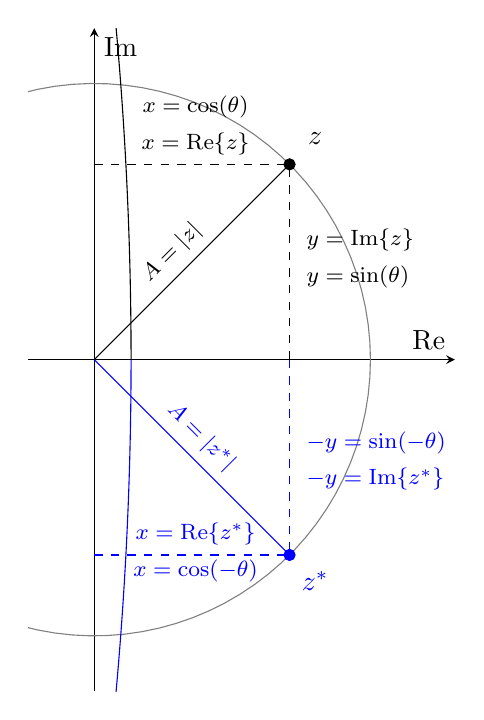
\begin{tikzpicture}
      \begin{axis}[axis equal, ymin=-1.8,xmin=-0.2,ymax=1.8,xmax=1.8,  ticks=none,
          xlabel=$\mathrm{Re}$,
          ylabel=$\mathrm{Im}$, axis lines = center, width=7cm, height=10cm]

        \addplot [gray,domain=0:2*pi,samples=100]({1.5*cos(deg(x))},{1.5*sin(deg(x))});

        \addplot [black, mark = *] coordinates {( {1.5*cos(45)}, {1.5*sin(45)} )} {};
        \addplot [blue, mark = *] coordinates {( {1.5*cos(-45)}, {1.5*sin(-45)} )} {};        
        %   \addplot [black, mark = *] coordinates {( {1.5*cos(-60)}, {1.5*sin(-60)} )} {};   

        \addplot [black] coordinates { (0,0) ( {1.5*cos(45)}, {1.5*sin(45)} ) };

        \addplot [blue] coordinates { (0,0) ( {1.5*cos(-45)}, {1.5*sin(-45)} ) };

        \addplot [dashed,black] coordinates { ({1.5*cos(45)},0) ( {1.5*cos(45)}, {1.5*sin(45)} ) };

        \addplot [dashed,blue] coordinates { ({1.5*cos(45)},0) ( {1.5*cos(45)}, {1.5*sin(-45)} ) };

        \addplot [dashed,black] coordinates { (0,{1.5*sin(45)}) ( {1.5*cos(45)}, {1.5*sin(45)} ) };

        \addplot [dashed,blue] coordinates { (0,{1.5*sin(-45)}) ( {1.5*cos(45)}, {1.5*sin(-45)} ) };

        \draw[draw=black] (axis cs:0.2,0.00) arc [radius={transformdirectionx(0.2)},start angle=0,end angle=45]
        node[midway,right,inner sep=3pt,font={\footnotesize}]{$\theta=\angle z$};

        \draw[draw=blue] (axis cs:0.2,0.00) arc [radius={transformdirectionx(0.2)},start angle=0,end angle=-45]
        node[midway,right,inner sep=3pt,font={\footnotesize}]{{\color{blue}$-\theta=\angle z^*$}};

        \node at (axis cs:0.55,1.06) [above, font={\footnotesize}]{$x=\mathrm{Re}\{z\}$};
        \node at (axis cs:0.55,1.26) [above, font={\footnotesize}]{$x=\cos(\theta)$};        
        \node at (axis cs:0.55,-1.06) [above, font={\footnotesize}]{{\color{blue}$x=\mathrm{Re}\{z^*\}$}};
        \node at (axis cs:0.55,-1.26) [above, font={\footnotesize}]{{\color{blue}$x=\cos(-\theta)$}};                

        \node at (axis cs:1.1,0.65) [right, font={\footnotesize}]{$y=\mathrm{Im}\{z\}$};
        \node at (axis cs:1.1,0.45) [right, font={\footnotesize}]{$y=\sin(\theta)$};        
        \node at (axis cs:1.1,-0.65) [right, color=blue, font={\footnotesize}]{$-y=\mathrm{Im}\{z^*\}$};
        \node at (axis cs:1.1,-0.45) [right, color=blue, font={\footnotesize}]{$-y=\sin(-\theta)$};        

        \node at (axis cs:1.2,1.2) {$z$};
        \node at (axis cs:1.2,-1.2) {{\color{blue}$z^*$}};        

        \node at (axis cs:0.5,0.5) [above,rotate=45,font={\footnotesize}]{$A=|z|$};
        \node at (axis cs:0.5,-0.5) [above,rotate=-45,font={\footnotesize}]{{\color{blue}$A=|z^*|$}};        
      \end{axis}
    \end{tikzpicture}
  \end{center}
  \caption{The polar representation of a complex number $z=x+iy =Ae^{i\theta}$ and its conjugate $z^* = x - iy = A e^{-i\theta}$}
  \label{fig:polar_euler}
\end{marginfigure}

\if 0
  \begin{marginfigure}

    \begin{center}
      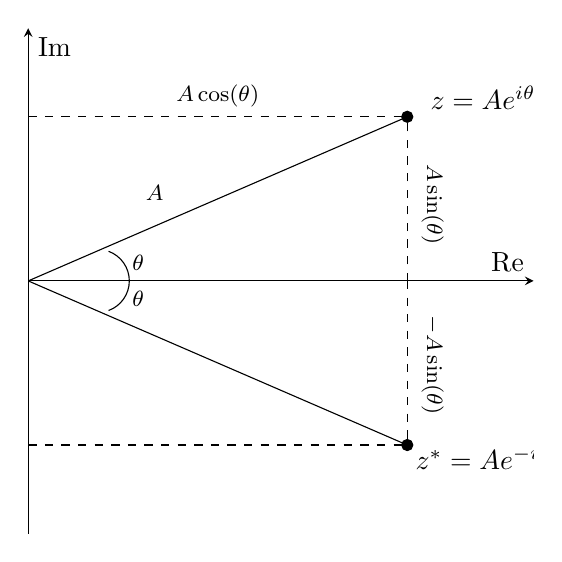
\begin{tikzpicture}
        \begin{axis}[
            ymin=-2.0,
            xmin=0.0,
            ymax=2.0,
            xmax=1.0,
            ticks=none,
            xlabel=$\mathrm{Re}$,
            ylabel=$\mathrm{Im}$,
            axis lines = center,
            width=8cm, height=8cm]
          \addplot [black, mark = *] coordinates {( {1.5*cos(60)}, {1.5*sin(60)} )} {};
          \addplot [black, mark = *] coordinates {( {1.5*cos(-60)}, {1.5*sin(-60)} )} {};

          \addplot [black] coordinates { (0,0) ( {1.5*cos(60)}, {1.5*sin(60)} ) };
          \addplot [dashed,black] coordinates { ({1.5*cos(60)},0) ( {1.5*cos(60)}, {1.5*sin(60)} ) };
          \addplot [dashed,black] coordinates { (0,{1.5*sin(60)}) ( {1.5*cos(60)}, {1.5*sin(60)} ) };

          \addplot [black] coordinates { (0,0) ( {1.5*cos(-60)}, {1.5*sin(-60)} ) };
          \addplot [dashed,black] coordinates { ({1.5*cos(-60)},0) ( {1.5*cos(-60)}, {1.5*sin(-60)} ) };
          \addplot [dashed,black] coordinates { (0,{1.5*sin(-60)}) ( {1.5*cos(-60)}, {1.5*sin(-60)} ) };

          %  \draw [black,-] (0,0) arc [radius=0.5,start angle=0,end angle=60];
          \draw[draw=black] (axis cs:0.2,0) arc [radius=0.4cm,start angle=0,end angle=70]
          node[midway,right,inner sep=3pt,font={\footnotesize}]{$\theta$};

          \draw[draw=black] (axis cs:0.2,0) arc [radius=0.4cm,start angle=0,end angle=-70]
          node[midway,right,inner sep=3pt,font={\footnotesize}]{$\theta$};

          \node at (axis cs:0.375,1.3) [above, font={\footnotesize}]{$A\cos(\theta)$};
          \node at (axis cs:0.8,1.0) [right, rotate=-90, font={\footnotesize}]{$A\sin(\theta)$};
          \node at (axis cs:0.8,-0.20) [right, rotate=-90, font={\footnotesize}]{$-A\sin(\theta)$};

          \node at (axis cs:0.9,1.45) {$z= A e^{i\theta}$};
          \node at (axis cs:0.9,-1.4) {$z^* = A e^{-i\theta}$};
          \node at (axis cs:0.25,0.7) [font={\footnotesize}]{$A$};

        \end{axis}
      \end{tikzpicture}
    \end{center}
    \caption{A complex number $z=x+iy =Ae^{i\theta}$, and it's complex conjugate $z^* = x-iy = A e^{-i\theta}$.}
    \label{fig:conjugate}
  \end{marginfigure}
\fi
% complex numbers

\newthought{\index{Euler's formula}{Euler's formula} relates an arbitrary \index{complex
  number}{complex
  number} $z \in \mathbb{C}$ to an exponential function of the \index{natural
  number}{natural
  number} $e$} and the $\sin$ and $\cos$ trigonometric functions as follows:
\begin{equation}
  \boxed{
    z = x + iy = A e^{i\theta} = A[\cos(\theta)+i\sin(\theta)]
  }\,\,.
  \label{eq:eulerintro}
\end{equation}
This formula is useful, as it provides a relationship between the Cartesian and \index{polar representation}{polar representation} of a \index{complex number}{complex number}\footnote{The \emph{\index{proof of Euler's formula}{proof of Euler's formula}} can be obtained in several different ways. We will use the derivative method demonstrated out by Youtuber MichaelPennMath. It relies on investigating that $f(\theta)=e^{-i\theta}e^{i\theta}=1$ holds when $e^{i\theta}=cos\theta + i\sin\theta$. Consider the following function:
\[
f(\theta) = e^{-i\theta}[\cos(\theta)+i\sin(\theta)].
\]
We know that $f(0)=1$ just by relying on $e^0=0$, $\cos(0)=1$ and $\sin(0)=0$. The derivative of this function is zero everywhere:
\begin{align*}
\frac{df}{d\theta} =& e^{-i\theta}[-\sin(\theta)+i\cos(\theta)] \\
&- i e^{-i\theta}[\cos(\theta)+i\sin(\theta)] \\
= & 0
\end{align*}
From this, we know that $f(\theta) = f(0) = 1$. The function is constant everywhere.

With a little bit of algebra, we can see that because $f(\theta)=1$, then $e^{i\theta}=e^{i\theta} f(\theta)$, and thus
\[
e^{i\theta} = \cos(\theta) + i\sin(\theta).
\]
This proves Euler's formula.}.



In this formula, $A = |z|=\sqrt{x^2 + y^2}$ is the absolute value of the complex number $z$. This is sometimes called the \emph{\index{magnitude}{magnitude}} or
\emph{\index{modulus}{modulus}} of $z$.

The angle $\theta$ can be obtained with simple geometry
$\theta=\tan^{-1}(y/x)$. The angle is also sometimes called the \emph{\index{argument}{argument}} of $z$. We'll use the following notation to denote the argument of a complex number: $\angle z = \theta = \tan^{-1}(y/x)$. In some other texts you might run into the following notation: $\angle z = \mathrm{Arg\{z\}}$.

It is worth pointing out here is that it is possible to add an integer
multiple of $2\pi$ to $\theta$ and still get the same complex number:
\begin{equation}
  A e^{i\theta} = A e^{i(\theta + 2\pi k)}
\end{equation}
This is due to the fact that $e^{i2\pi k} = 1$, where
$k \in \mathbb{Z}$ is an arbitrary integer. The fact that there are
infinitely many different solutions to the argument of a complex
number is an important property, which will be encountered often in
signal processing. For example, the concept
of \emph{\index{aliasing}{aliasing}} of discretized signals, which will
encounter later on, occurs due to this this property.

The term $i$ in Equation \ref{eq:eulerintro} is the imaginary number, which has the following properties: $i=\sqrt{-1}$ and $i^2 = -1$. In engineering and programming, the symbol $j$ is also often used for the imaginary number instead of $i$. The Python programming language uses the symbol $j$, and to denote e.g., $z=2+5i$ in Python, you would use the code snippet \verb|z=2+5j|.   % I'll use $i$, but you can use whichever notation you prefer yourself.

The geometric representation of a complex number is shown in
Figure \ref{fig:polar_euler}, which shows the real and imaginary
components of a complex number in a two-dimensional coordinate system-- the complex plane.

The complex exponential obey the same exponentiation rules as the real exponential function:
\begin{equation}
  \boxed{
  e^{z_{1}}e^{z_{2}} = e^{z_{1}+z_{2}}
  }\,\,.
  \label{eq:complexexponentiation}
\end{equation}
for all complex numbers $z_{1},z_{2}\in\mathbb{C}$, moreover $(e^{z_{1}})^{z_{2}}=e^{z_{1}z_{2}}$.

\newthought{The conjugate $z^*$} of complex number $z$ is defined as:
\begin{align}
  z^* & = x - iy                         \\
      & =A[\cos(\theta)-i\sin(\theta)]   \\
      & =A[\cos(-\theta)+i\sin(-\theta)] \\
      & =A e^{-i\theta}\,\,.
\end{align}
The conjugation operation flips the sign of the imaginary
component. The geometric interpretation of the \index{complex conjugate}{complex conjugate} is
shown in Figure \ref{fig:polar_euler}.  We'll use the superscript star notation to denote the conjugation operator.

\newthought{The complex conjugate can be used to obtain the magnitude of the complex number}:
\begin{equation}
\boxed{
|z| = \sqrt{z z^*} = \sqrt{x^2 + y^2}.
}
\end{equation}
%as $zz^*=(x+iy)(x-iy)=x^2+y^2$
%or $zz^* = |z|e^{i\theta}|z|e^{-i\theta}=|z|^2$.

\newthought{A complex conjugate can also be used to select the real and imaginary
  components of a complex number} as follows:
\begin{equation}
\boxed{
  \Re{z}  = \frac{1}{2}(z+z^*)=x
  \label{eq_conj}
  }
\end{equation}
and 
  \begin{equation}
\boxed{
  \Im{z}  = \frac{1}{2i}(z-z^*)=y
  \label{eq_conj2}
  }
\end{equation}
These formulas are often encountered when dealing with real-valued signals. It is often easier to algebraically to manipulate signals of the form $Ae^{i\theta}$, and after the calculations are done, it is simply a matter of using equation \ref{eq_conj} to extract the real component of the signal from its complex representation. 

\newthought{The use of a sum of a complex number and it's conjugate can be used to relate the exponent function to a cosine and sine function}. Using Euler's formula for $z=e^{i\theta}$ and Equations \ref{eq_conj} and \ref{eq_conj2}, we can obtain:
\begin{equation}
\boxed{
  \cos(\theta)  = \frac{1}{2}\left(e^{i\theta} + e^{-i\theta}\right) \label{inveul0}
  }
  \end{equation}
\begin{equation}
\boxed{
  \sin(\theta)  = \frac{1}{2i}\left(e^{i\theta} - e^{-i\theta}\right). \label{inveul}
  }
\end{equation}
These relations are sometimes called the \emph{\index{inverse
    Euler}{inverse Euler}} relations. You'll encounter these formulas when converting a $\cos$ or $\sin$ function into two complex exponent functions. The first step of a signal processing related calculation involving real-valued signals is often making this conversion, as functions of the form $A e^{i\theta}$ are significantly easier to deal with.

\begin{marginfigure}
  \begin{center}
\includegraphics[width=\textwidth]{ch03/figures/compmult.png}
\end{center}
  \caption{Multiplication of two complex numbers (TBD: cleanup figure)}
  \label{fig:comp_mult}
\end{marginfigure}

\newthought{Complex multiplication can be viewed as multiplication of magnitudes and summation of phases}. Let's express two complex numbers in polar form as $z_1=A_1e^{i\theta_1}$ and $z_2=A_2e^{i\theta_2}$. We can now see that multiplication with complex numbers has an intuitive interpretation.
\begin{equation}
  z_1 z_2 = A_1 e^{i\theta_1} A_2 e^{i\theta_2} = \underbrace{A_1
    A_2}_{A_3} \underbrace{e^{i(\theta_1 + \theta_2)}}_{e^{i\theta_3}} =
  A_3 e^{i\theta_3} \,\,.
\end{equation}
When multiplying two numbers, the resulting angle is a sum of the two angles $\theta_3=\theta_1 + \theta_2$, which can be also seen as a rotation of the point indicated by a complex number $z_1$ by angle $\theta_2$ on the complex plane. The new magnitude is the magnitudes of the two numbers multiplied together $A_3=A_1A_2$. Figure \ref{fig:comp_mult} demonstrates multiplication geometrically on the complex plane.

\begin{figure}
  \begin{center}
    \includegraphics[width=\textwidth]{code/006_spiral/spiral.png}
  \end{center}
  \caption{A spiral is formed by evaluating $z^n$ with integer values of $n$ between $0$ and $41$. In this case $z = 0.92 e^{i 2\pi /20}$. The parametric curve $e^{i\theta}$ with $\theta \in \mathbb{R}$ draws a circle in the complex plane, which is depicted with a gray color. The code that generated this plot can be found in \texttt{006\_spiral/spiral.py}.}
  \label{fig:spirals}
\end{figure}

\newthought{Raising a complex number to the $n$th power} can be seen as exponential scaling and rotation. Consider a complex number
\begin{equation}
  z = A e^{i\theta}
\end{equation}
where $A \in \mathbb{R}_{\ge 0}$ and $\theta \in \mathbb{R}$. If we raise this to the $n$th power, we get:
\begin{equation}
  z^n = A^n e^{i\theta n} = A^n [\cos(\theta n) + i \sin(\theta n)]\,\,.
\end{equation}
Scaling and rotation is demonstrated in Figure \ref{fig:spirals}.

\newthought{Here are some Python examples of complex number operations}.

\lstinputlisting[language=Python, caption={\texttt{008\_complex\_ops/ops\_example.py}}, label=lst:ex1]{code/008_complex_ops/ops_example.py}





\input{ch03/exercises3}
 \ifSpExerciseSol
 \input{ch03/solutions3}
 \fi
\fi

\ifSpSigSys
\chapter{Signals and Systems}
\input{ch04/text4}
\input{ch04/exercises4}
 \ifSpExerciseSol
 \input{ch04/solutions4}
 \fi
\fi

\ifSpElSig
\chapter{Elementary Signals}
%
% Continuous-time signals
% Commonly encountered special functions
% 
% - Dirac delta
% - Unit-step function
% - 
%
\newthought{There are two important elementary signals} which you will encounter
throughout signal processing: the \emph{\index{unit impulse}{unit
impulse}} $\delta(t)$ and the \emph{\index{unit step}{unit step}}
function $u(t)$. These are important functions, as we can use these
signals to represent any arbitrary signal. They play an \emph{especially
important role in defining signals in time domain}. If we know how a
linear time-invariant system modifes these functions, then we are able
to model how arbitrary signals behave. The unit impulse and unit step
function have both continuous-time and discrete-time versions.


\newthought{The unit impulse function $\delta(t)$} is a special distribution
function\footnote{The unit impulse function is also known as the
  \emph{\index{Dirac delta function}{Dirac delta function}}, after physicist Paul Dirac,
  who used this function for modeling the distribution of electrical point-charges (e.g., electrons and protons)},
which is infinitely narrow, non-zero valued only at $t=0$.
And when you integrate over this function, the result will be 1.

It is possible to define $\delta(t)$ in several ways as a limit of
functions with a well-defined area and width $\sigma$.  I'll use the
Gaussian density function:
\begin{equation}
  \delta_\sigma(t) = \frac{1}{\sqrt{2\pi \sigma^2}}e^{-\frac{t^2}{2\sigma^2}}\,\,.
\end{equation}
The \index{Gaussian density function}{Gaussian density function} is shown in Figure \ref{fig:gauss_dens} for
two different standard deviations $\sigma_1$ and $\sigma_2$.
The smaller the value of $\sigma$, the more narrow the function is.

\begin{marginfigure}
  \begin{center}
    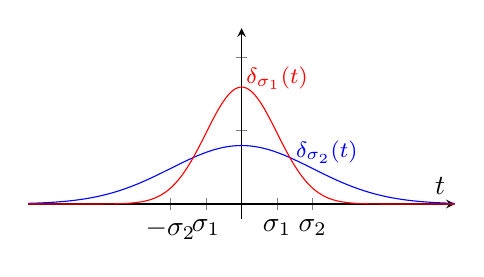
\begin{tikzpicture} \begin{axis}[width=7cm,height=4cm,ymin=-0.1,xmin=-3,ymax=1.2,xmax=3,
          yticklabels={,,}, xtick={-1,-0.5,0,0.5,1},
          xticklabels={$-\sigma_2$,$\sigma_1$,0,$\sigma_1$,$\sigma_2$},
          xlabel=$t$, axis lines = center]

        %\addplot +[dirac] coordinates {(1,1.4)};
        %\node at (axis cs:1.2,0.85) [below, font={\footnotesize}]{$\delta(t-t_0)$};

        \node at (axis cs:1.2,0.5) [below, font={\footnotesize},color=blue]{$\delta_{\sigma_2}(t)$};
        \addplot[samples=400,mark=none,color=blue]{(1/sqrt(2*3.14))*exp(-x^2/2.0)};

        \node at (axis cs:0.5,1.0) [below, font={\footnotesize},color=red]{$\delta_{\sigma_1}(t)$};
        \addplot[samples=400,mark=none,color=red]{(1/sqrt(2*3.14*0.25))*exp(-x^2/(2.0*0.25))};


      \end{axis}
    \end{tikzpicture}
  \end{center}
  \caption{A Gaussian density function becomes a unit impulse $\delta(t)$
    when the width parameter approaches zero $\sigma \rightarrow 0$.}
  \label{fig:gauss_dens}
\end{marginfigure}
\pgfplotsset{
  dirac/.style={
      mark=triangle*,
      mark options={scale=2},
      ycomb,
      scatter,
      visualization depends on={y/abs(y)-1 \as \sign},
      scatter/@pre marker code/.code={\scope[rotate=90*\sign,yshift=-2pt]}
    }
}
\begin{marginfigure}[0cm]
  \begin{center}
    \begin{tikzpicture}
      \begin{axis}[width=7cm,height=4cm,ymin=0,xmin=-0.5,ymax=1.1,xmax=1.5,
          yticklabels={,,},
          xtick={1},
          xticklabels={$\tau$},
          xlabel=$t$, axis lines = center]

        \addplot +[dirac] coordinates {(1,1)};
        \node at (axis cs:0.68,1) [below, font={\footnotesize}]{$\delta(t-\tau)$};

      \end{axis}
    \end{tikzpicture}
  \end{center}

  \caption{A unit impulse is typically depicted with a vertical arrow. 
  A unit impulse $\delta(t-\tau)$ is centered at $t=\tau$. 
  This is the only value of $t$ where the unit impulse is non-zero.}
  \label{fig:uparrow}
\end{marginfigure}

As a result of how the function is defined, an integral over
$\delta_{\sigma}(t)$ is always unity. This is perhaps not a surprise,
as this function is used in statistics as a probability density
function:
\begin{equation}
  \int_{-\infty}^{\infty}\delta_\sigma(t)dt = 1 \,\,.
\end{equation}
The Dirac delta function $\delta(t)$ can be thought of as the limit
when the standard deviation of this distribution approaches zero:
\begin{equation}
  \lim_{\sigma\rightarrow 0}  \int_{-\infty}^{\infty} \delta_\sigma(t) dt = \int_{-\infty}^{\infty} \delta(t) dt = 1
\end{equation}
For the sake of this course, we are not going to need to
mathematically investigate the limit of this function. However, it is
hopefully not difficult to convince yourself that the function becomes
more and more narrow as $\sigma \rightarrow 0$, and that for all
values of $\sigma$, the integral evaluates to unity.

But what does the function $\delta(t)$ look like? It is infinitely
narrow, with only one non-zero value at zero. The equation below is
not strictly a rigorous mathematical definition, but it gives you an
idea:
\begin{equation}
  \delta(t) = \left\{ \begin{array}{ccc}
    \infty & \mathrm{when} & t=0     \\
    0      & \mathrm{when} & t \ne 0
  \end{array}\right.
\end{equation}
When plotting this function, it is customary to utilize an up arrow,
as shown in Figure \ref{fig:uparrow}. The figure also demonstrates how
it is possible to shift the location of the peak by subtracting a
constant $\tau$ from the argument of the function.

\begin{marginfigure}[0cm]
  \begin{center}
    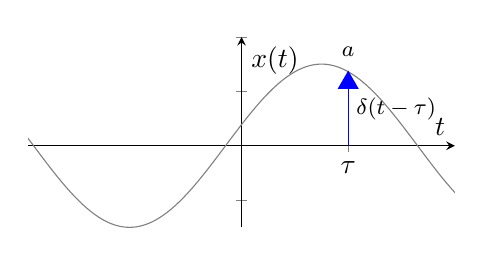
\begin{tikzpicture}
      \begin{axis}[width=7cm,height=4cm,ymin=-1.5,xmin=-2,ymax=2,xmax=2,         yticklabels={,,},
          xtick={1.0},
          xticklabels={$\tau$},
          %        xticklabels={,,},
          ylabel=$x(t)$,
          xlabel=$t$, axis lines = center]

        \addplot +[dirac] coordinates {(1,1.36)};
        \node at (axis cs:1.45,1.05) [below, font={\footnotesize}]{$\delta(t-\tau)$};
        %\node at (axis cs:0.5,1.8) [below, font={\footnotesize}]{$x(t)$};

        \node at (axis cs:1.0,2.0) [below, font={\footnotesize}]{$a$};

        %\addplot[samples=400,mark=none,color=gray]{0.1*x*x*x-0.7*x*x + x + 1};
        \addplot[samples=400,mark=none,color=gray]{1.5*sin(100*x+15)};

      \end{axis}
    \end{tikzpicture}
  \end{center}
  \caption{The unit impulse ``selects'' the value of a continuous-time signal $x(\tau)=a$.}
\end{marginfigure}

\begin{marginfigure}
  \begin{center}
    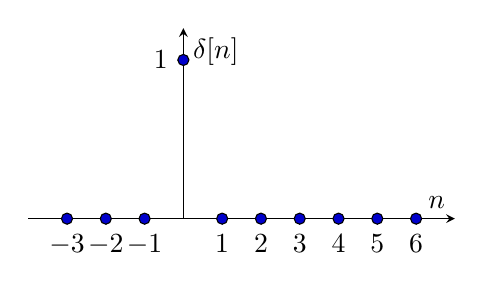
\begin{tikzpicture}
      \begin{axis}[width=7cm,height=4cm,ymin=0,xmin=-4,ymax=1.2,xmax=7,
          xtick={-3,-2,-1,0,1,2,3,4,5,6},
          ytick={0,1,2,3},
          ylabel={$\delta[n]$},
          xlabel={$n$}, axis lines = center]
        \addplot+[ycomb,color=black] plot coordinates {(-3,0) (-2,0) (-1,0) (0,1) (1,0) (2,0) (3,0) (4,0) (5,0) (6,0)};
      \end{axis}
    \end{tikzpicture}
  \end{center}
  \caption{The discrete-time unit impulse.}
  \label{fig:udensdisc}
\end{marginfigure}

The main application of the unit impulse function in signal processing is 
selecting or ``sampling'' a value of a signal. This is also sometimes referred to 
as the \emph{\index{sifting}{sifting}} property. Consider a function $x(t)$ which 
has the value $x(\tau) = a$. If we integrate over the function $x(t)\delta(t-\tau)$, 
we obtain:
\begin{equation}
  \int_{-\infty}^{\infty}x(t)\delta(t-\tau) dt = x(\tau) = a\,\,.
\end{equation}
This type of integral will often appear when relating a continuous-time theory to a discrete-time theory.
If you are still having a difficult time convincing yourself why the integral above results 
in the value it does, try thinking about it through the limit:
\begin{equation}
  \lim_{\sigma\rightarrow 0}\int_{-\infty}^{\infty}x(t)\delta_{\sigma}(t-\tau) dt = x(\tau) = a\,\,.
\end{equation}
The Dirac delta function is for the most part, used in this course
inside an integral, and we will never need to deal with the
singularity ($\infty$).

\if 0
  \begin{equation}
    \lim_{\sigma \rightarrow 0} \delta_{\sigma}(t) = \delta(t)\,\,,
  \end{equation}
  where the uniform density function $\delta_{\sigma}(t)$ is defined as:
  \begin{equation}
    \delta_{\sigma}(t) =\left\{ \begin{array}{cl}
      \sigma^{-1}, & -\frac{1}{2}\sigma < t < \frac{1}{2}\sigma \\
      0,           & \mathrm{otherwise}.\end{array}
    \right.\,\,.
  \end{equation}
  This function is identical to the probability density function of a
  uniformly distributed random variable. The function
  $\delta_{\sigma}(t)$ is depicted for two different values of $\sigma$
  in Figure \ref{fig:udens}. It is a rectangle with width $\sigma$ on
  the t-axis and an amplitude of $1/\sigma$:
  \begin{marginfigure}
    \begin{center}
      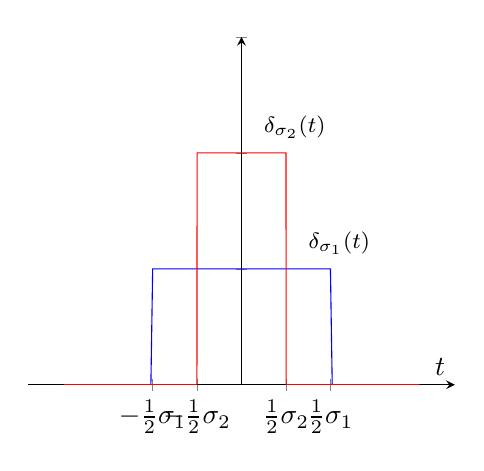
\begin{tikzpicture}
        \begin{axis}[width=7cm,height=6cm,ymin=0,xmin=-1.2,ymax=3.0,xmax=1.2,         yticklabels={,,},
            xtick={-0.5,-0.25,0.25,0.5},
            xticklabels={$-\frac{1}{2}\sigma_1$,$-\frac{1}{2}\sigma_2$,$\frac{1}{2}\sigma_2$,$\frac{1}{2}\sigma_1$},
            xlabel=$t$, axis lines = center]
          \addplot[color=blue] plot coordinates {(-1,0) (-0.51,0.0) (-0.5,1.0)(0.5,1.0) (0.51,0.0) (1,0)};
          \addplot[color=red] plot coordinates {(-1,0) (-0.251,0.0) (-0.25,2.0)(0.25,2.0) (0.251,0.0) (1,0)};

          \node at (axis cs:0.55,1.4) [below, font={\footnotesize}]{$\delta_{\sigma_1}(t)$};

          \node at (axis cs:0.3,2.4) [below, font={\footnotesize}]{$\delta_{\sigma_2}(t)$};
        \end{axis}
      \end{tikzpicture}
    \end{center}
    \caption{A rectangular pulse signal becomes a unit impulse when the width parameter $\sigma_1 \rightarrow 0$ approaches zero.}
    \label{fig:udens}
  \end{marginfigure}
\fi

%\newthought{The unit impulse can also be defined as an infinitely narrow Gaussian density function}:

\newthought{The discrete-time unit impulse $\delta[n]$} is defined as:
\begin{equation}
  \delta[n] = \left\{\begin{array}{cl}
    1 & ~~~ n = 0   \\
    0 & ~~~ n \ne 0 \\
  \end{array}
  \right.\,\,.
\end{equation}
The discrete-time unit impulse signal is shown in
Figure \ref{fig:udensdisc}. In most cases, the discrete-time unit
impulse serves a similar function as its continuous-time
equivalent. It is often theoretically advantageous to study linear
systems by representing an arbitrary signal $x[n]$ as a sum of time
shifted and scaled unit impulses:
\begin{equation}
x[n] = \sum_k x[k] \delta[n-k].
\end{equation}
This may seem like a unnecessarily complicated way of expressing a
signal, but the advantage is that it simplifies the study of systems,
allowing us to focus on analyzing what a linear system does to a time
shifted unit impulse $\delta[n-k]$.

%\newpage
%\subsection{Unit step}


\newthought{The unit step function} can be defined as
follows\footnote{This function is also called the
  \index{Heaviside-function}{Heaviside-function}, after Oliver
  Heaviside, who used this function to model signals used in
  telecommunications.}:
\begin{equation}
  u(t) = \left\{\begin{array}{cl}
    0 & ~~~ t < 0   \\
    1 & ~~~ t \ge 0 \\
  \end{array}
  \right. \,\,.
\end{equation}
It is a step-like function, which abruptly transitions to 1 at
zero. The following figure depicts the unit step function. Notice
that there is a discontinuity at $t=0$. %There are different variants
%of the unit step function that treat this discontinuity differently.
\tikzstyle{int}=[draw, minimum size=2em]
\tikzstyle{init} = [pin edge={to-,thin,black}]
\begin{marginfigure}[0cm]
  \begin{center}

    \begin{tikzpicture}
      \begin{axis}[width=7cm,height=4cm,ymin=0,xmin=-2,ymax=1.3,xmax=2,
          ytick={0,1},
          xtick={0},
          yticklabels={0,1},
          xticklabels={0},
          ylabel=$u(t)$,
          xlabel=$t$,
          axis y line=middle, axis x line=bottom]


        % \addplot[color=blue] plot coordinates {(-3,0) (0.00001,0) (0.0,1.0) (10,1.0) };
        %\addplot[color=blue] plot coordinates {(-3,0) (0.00001,0)};
        %\addplot[color=blue] plot coordinates {(0.0,1.0) (10,1.0)};
        \addplot[color=red] plot coordinates {(-3,0) (0.00001,0)};
        \addplot[color=red] plot coordinates {(0.0,1.0) (10,1.0)};
        \addplot+[only marks,mark=o,color=red] plot coordinates {(0,0) (0.0,1)};
        \node at (axis cs:-1.8,1.3) [below, font={\footnotesize}]{a)};

        %\addplot[color=red] plot coordinates {(-3,0) (0.99,0) (1.0,1.0) (10,1.0) };
        %\addplot[color=red] plot coordinates {(-1,0) (-0.251,0.0) (-0.25,2.0)(0.25,2.0) (0.251,0.0) (1,0)};

        %\node at (axis cs:1.0,1.0) [below, font={\footnotesize}]{$u(t-\tau)$};

      \end{axis}
    \end{tikzpicture}
    \begin{tikzpicture}
      \begin{axis}[width=7cm,height=4cm,ymin=0,xmin=-1,ymax=1.3,xmax=2,
          ytick={0,1},
          yticklabels={0,1},
          xtick={0,1},
          xticklabels={0,$L$},
          ylabel=$u(t)-u(t-L)$,
          xlabel=$t$,
          axis y line=middle, axis x line=bottom]
          
        \node at (axis cs:-0.8,1.3) [below, font={\footnotesize}]{b)};
        
        \addplot[color=blue] plot coordinates {(-3,0) (0.00001,0) (0.0,1.0) (1.0,1) (1.0,0) (10,0.0)};
        %\addplot+[only marks,mark=o,color=blue] plot coordinates {(0,0) (0.0,1)};
        %\addplot[color=red] plot coordinates {(-1,0) (-0.251,0.0) (-0.25,2.0)(0.25,2.0) (0.251,0.0) (1,0)};
      \end{axis}
    \end{tikzpicture}    
  \end{center}
  \caption{a) The unit step function $u(t)$ shown in blue transitions from 0 to 1 at the origin. b) Rectangular function expressed using two unit step functions.}
  \label{fig:rect_fun}
\end{marginfigure}


The unit step function can be used to create a \index{rectangular function}{rectangular function}
$\mu_L(t)$ of a certain length $L$. Here are two ways that this can be
done:
\begin{align*}
  \mu_L(t) & = u(t)-u(t-L)       \\
                    & = u(t) u(L-t) \,\,.
\end{align*}
Figure \ref{fig:rect_fun} shows a plot of the rectangular
function. This type of function appears, e.g., when dealing with ideal
filters that only select spectral components that lie within a
specific band of frequencies. Rectangular function can also be used to
model signal carrying radar or telecommunications signals, which have
a constant value over a specific time period. Consider e.g., the
following example, which happens to be the three bit Barker code used
for radar pulse compression:
\begin{equation}
x(t) = \sum_{k=0}^{2} b_k \mu_L(t-kL)
\end{equation}
  \begin{figure}
    \begin{center}
      \begin{tikzpicture}
        \begin{axis}[width=\textwidth,height=4cm,ymin=-1.3,xmin=-0.5,ymax=1.3,xmax=4.5,
            ytick={-1,0,1},
            yticklabels={-1,0,1},
            xtick={0,1,2,3,4},
            xticklabels={0,$L$,$2L$,$3L$,$4L$},
            axis y line=middle,
            axis x line=middle,
            xlabel=$t$]

          \addplot[color=blue] plot coordinates {(-3,0) (0,0.0) (0.0,1.0) (1,1.0) (1,0.0)};
          \addplot[color=blue] plot coordinates { (1,0.0) (1.0,-1.0) (2,-1.0) (2,0)};
          \addplot[color=blue] plot coordinates { (2,0) (2.0,-1.0) (3,-1.0) (3,0.0) (4,0)};

          %\addplot[color=red] plot coordinates {(-1,0) (-0.251,0.0) (-0.25,2.0)(0.25,2.0) (0.251,0.0) (1,0)};

          \node at (axis cs:0.5,1.0) [below, font={\footnotesize}]{$b_0=1$};
          \node at (axis cs:1.5,1.0) [below, font={\footnotesize}]{$b_1=-1$};
          \node at (axis cs:2.5,1.0) [below, font={\footnotesize}]{$b_2=-1$};          

        \end{axis}
      \end{tikzpicture}
    \end{center}
    \caption{A three-bit Barker code represented with the help of three rectangular functions.}
      \label{fig:rectbarker}
  \end{figure}

\if 0
\begin{marginfigure}[-0cm]
  \begin{center}
    \begin{tikzpicture}
      \begin{axis}[width=7cm,height=4cm,ymin=0,xmin=-1,ymax=1.3,xmax=2,
          ytick={0,1},
          yticklabels={0,1},
          xtick={0,1},
          xticklabels={0,$L$},
          ylabel=$u(t)-u(t-L)$,
          xlabel=$t$,
          axis y line=middle, axis x line=bottom]

        \addplot[color=blue] plot coordinates {(-3,0) (0.00001,0) (0.0,1.0) (1.0,1) (1.0,0) (10,0.0)};
        %\addplot+[only marks,mark=o,color=blue] plot coordinates {(0,0) (0.0,1)};
        %\addplot[color=red] plot coordinates {(-1,0) (-0.251,0.0) (-0.25,2.0)(0.25,2.0) (0.251,0.0) (1,0)};
      \end{axis}
    \end{tikzpicture}
  \end{center}
  \caption{A rectangular function that is obtained using a unit step function $u(t)-u(t-L)$.}
  \label{fig:rect_fun}
\end{marginfigure}
\fi
\if 0
  \newthought{It is possible to relate the unit step and the unit impulse functions}. 
   The unit step function can be thought of as an integral over the unit impulse over the interval $[-\infty,t]$:
  \begin{equation}
    u(t) = \int_{-\infty}^{t} \delta(\tau) d\tau \,\,.
  \end{equation}
  The above suggests that we can relate the derivative of the unit step
  function to the unit impulse, which is true.

  Because the unit-step function is also a special function, which has a
  discontinuity, we need to study the time-derivative by investigating
  the limit of a differentiable function.  Consider the following
  cumulative distribution function:
  \begin{equation}
    u_{\Delta}(t) = \left\{\begin{array}{cl}
      0,                 & t < 0            \\
      \frac{1}{\Delta}t, & 0 \le t < \Delta \\
      1,                 & t \ge \Delta.
    \end{array}
    \right\} \,\,.
  \end{equation}

  \begin{marginfigure}
    \begin{center}
      \begin{tikzpicture}
        \begin{axis}[width=7cm,height=6cm,ymin=0,xmin=-0.5,ymax=1.3,xmax=2,
            ytick={0,1},
            yticklabels={0,1},
            xtick={0,0.5},
            xticklabels={0,$\sigma$},
            axis y line=middle,
            axis x line=bottom,
            xlabel=$t$]

          \addplot[color=blue] plot coordinates {(-3,0) (0,0.0) (0.5,1.0) (5,1.0)};
          %\addplot[color=red] plot coordinates {(-1,0) (-0.251,0.0) (-0.25,2.0)(0.25,2.0) (0.251,0.0) (1,0)};

          \node at (axis cs:0.2,1.0) [below, font={\footnotesize}]{$u_{\sigma}(t)$};

        \end{axis}
      \end{tikzpicture}
    \end{center}
    \caption{Imagine that the unit step function jumps from $0$ to $1$ in time $\Delta t = \sigma$, 
    and as $\sigma \rightarrow 0$, the jump becomes a vertical line.}
  \end{marginfigure}
  The unit step function in this case is:
  \begin{equation}
    u(t) = \lim_{\sigma \rightarrow 0}  u_{\sigma}(t) \,\,.
  \end{equation}
  The derivative of $u_{\sigma}(t)$ is defined piecewise as:
  \begin{equation}
    \delta_{\sigma}(t) = \frac{d}{dt}u_{\sigma}(t) =\left\{
    \begin{array}{cl}
      0,                & t<0                \\
      \frac{1}{\sigma}, & 0\le t < \sigma    \\
      0,                & \mathrm{otherwise}
    \end{array}
    \right\} \,\,.
  \end{equation}
  At the limit $\sigma\rightarrow 0$, the derivative becomes the Dirac-delta:
  \begin{equation}
    \lim_{\sigma \rightarrow 0 } \frac{d}{dt}u_{\sigma}(t) = \lim_{\sigma \rightarrow 0 }\delta_{\sigma}(t) = \delta(t) \,\,.
  \end{equation}
  We can thus treat $u(t)$ as a cumulative distribution function of a
  random variable that only has a non-zero probability density at
  $t=0$. With this definition, it is possible to relate the unit impulse
  with the unit step function:
  \begin{equation}
    \boxed{
      \delta(t) = \frac{d}{dt}u(t)
    } \,\,.
  \end{equation}
\fi

\newthought{The discrete-time unit step $u[n]$ function} is defined as:
\begin{equation}
  u[n] = \left\{\begin{array}{cl}
    0 & ~~~ n < 0   \\
    1 & ~~~ n \ge 0 \\
  \end{array}
  \right.\,\,.
\end{equation}
The discrete-time unit step function is shown in Figure \ref{fig:dt_ustep}.

\begin{marginfigure}[0cm]
  \begin{center}
    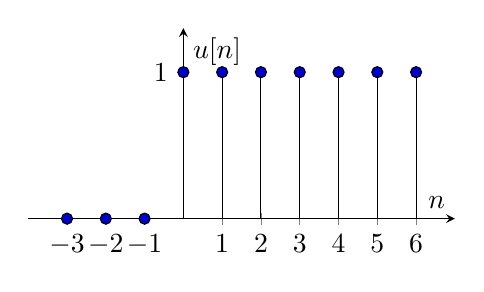
\begin{tikzpicture}
      \begin{axis}[width=7cm,height=4cm,ymin=0,xmin=-4,ymax=1.3,xmax=7,
          xtick={-3,-2,-1,0,1,2,3,4,5,6},
          ytick={0,1,2,3},
          ylabel={$u[n]$},
          xlabel={$n$}, axis lines = center]
        \addplot+[ycomb,color=black] plot coordinates {(-3,0) (-2,0) (-1,0) (0,1) (1,1) (2,1) (3,1) (4,1) (5,1) (6,1)};
      \end{axis}
    \end{tikzpicture}
  \end{center}
  \caption{A discrete-time unit step function.}
  \label{fig:dt_ustep}
\end{marginfigure}




\input{ch05/exercises5}
 \ifSpExerciseSol
 \input{ch05/solutions5}
 \fi
\fi

\ifSpSin
\chapter{Sinusoidal Signals}
\newthought{A \index{complex sinusoidal signal}{complex sinusoidal signal} is the
  elementary building block of the Fourier decomposition of a signal}.
This signal is fully determined by three parameters:
\index{amplitude}{amplitude} $A \in \mathbb{R}_{\ge 0}$, \index{phase}{phase} $\phi \in \mathbb{R}$ (rad), and
\index{angular frequency}{angular frequency} $\omega \in \mathbb{R}$ (rad/s).
\begin{equation}
  \boxed{
    z(t) = A e^{i(\omega t + \phi)} = A e^{i\phi} e^{i\omega t} = X e^{i\omega t}.
  }
\end{equation}
It is possible to combine phase and amplitude as one complex constant $X = Ae^{i\phi} \in \mathbb{C}$.
This constant contains information about the amplitude and phase of the signal.
Here $X$ is often referred to as a \emph{\index{phasor}{phasor}},
whenever $A$, $\omega$ and $\phi$ have no time-dependence.

\begin{marginfigure}
  \begin{center}
    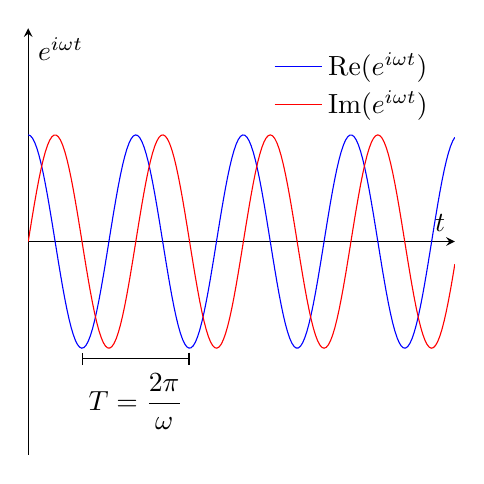
\begin{tikzpicture}
      \begin{axis}[domain=0:(2*6.23),
          width=7cm,
          height=7cm,
          ticks=none,
          axis lines = center,
          ymax=2,
          ymin=-2,
          samples=200,
          legend pos=north east,
          legend style={draw=none},
          xlabel={$t$},
          ylabel={$e^{i\omega t}$}]
        \addplot[blue] {cos(2*deg(x))};
        \addplot[red] {sin(2*deg(x))};

        \node at (axis cs:3.14,-1.5) {$\displaystyle{T=\frac{2\pi}{\omega}}$};
        \addplot [dimen] plot coordinates {(1.57,-1.1) (4.71,-1.1)};

        \legend{$\mathrm{Re}(e^{i\omega t})$,$\mathrm{Im}(e^{i\omega t})$}
      \end{axis}
    \end{tikzpicture}
  \end{center}
  \caption{A complex sinusoidal signal is the basic building block (basis function)
    in a Fourier decomposition of a signal. The fundamental period $T=2\pi/\omega$
    of this signal is also shown.}
  \label{fig:complex_sinusoid}
\end{marginfigure}

\begin{marginfigure}
  \begin{center}
    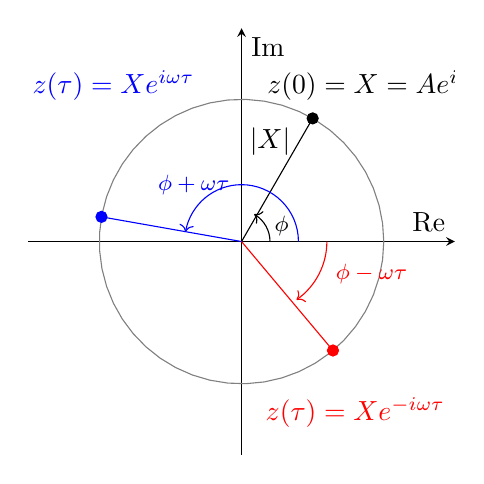
\begin{tikzpicture}
      \begin{axis}[axis equal, disabledatascaling,
          ymin=-1.5,xmin=-1.5,ymax=1.5,xmax=1.5, ticks=none,
          xlabel=$\mathrm{Re}$, ylabel=$\mathrm{Im}$, axis lines = center,
          width=7cm, height=7cm] \addplot
        [gray,domain=0:2*pi,samples=50]({cos(deg(x))},{sin(deg(x))});

        \addplot [black, mark = *] coordinates {( {cos(60)}, {sin(60)} )} {};
        \addplot [black] coordinates { (0,0) ( {cos(60)}, {sin(60)} ) };

        \addplot [blue, mark = *] coordinates {( {cos(170)}, {sin(170)} )} {};
        \addplot [blue] coordinates { (0,0) ( {cos(170)}, {sin(170)} ) };

        \addplot [red, mark = *] coordinates {( {cos(-50)}, {sin(-50)} )} {};
        \addplot [red] coordinates { (0,0) ( {cos(-50)}, {sin(-50)} ) };

        \draw[draw=black, ->] (axis cs:0.2,0) arc [radius=0.4cm,start angle=0,end angle=60]
        node[midway,right,inner sep=3pt,font={\footnotesize}]{$\phi$};

        %  \draw[draw=blue] (axis cs:1,0) arc [radius=0.5cm,start angle=60,end angle=120]
        %  
        \draw [blue, ->] (axis cs:0.4,0.0) arc [radius=0.4,start angle=0,end angle=170]
        node[midway,left,inner sep=6pt,font={\footnotesize}]{$\phi+\omega \tau$};

        \draw [red, ->] (axis cs:0.6,0.0) arc [radius=0.5,start angle=0,end angle=-55]
        node[midway,right,inner sep=6pt,font={\footnotesize}]{$\phi-\omega \tau$};

        \node at (axis cs:0.9,1.1) {$z(0)=X=Ae^{i\phi}$};

        \node at (axis cs:0.2,0.7) {$|X|$};

        \node[blue] at (axis cs:-0.9,1.1) {$z(\tau)=X e^{i\omega \tau}$};
        \node[red] at (axis cs:0.8,-1.2) {$z(\tau)=X e^{-i\omega \tau}$};
      \end{axis}
    \end{tikzpicture}
  \end{center}
  \caption{A complex sinusoidal signal on the complex plane can be seen as a
    point moving around a circle. For positive frequencies, the point rotates
    around the circle in counterclockwise direction. For negative frequencies, the rotation is clockwise.}
  \label{fig:rotating_phasor}
\end{marginfigure}

Using Euler's formula, we can express the \index{complex sinusoidal signal}{complex sinusoidal signal}
as a function of \index{$\cos$}{$\cos$} and \index{$\sin$}{$\sin$}:
\begin{equation}
  Ae^{i(\omega t + \phi)}= A[\cos(\omega t + \phi) + i \sin(\omega t + \phi)].
\end{equation}
With this formulation, it is apparent that the real and imaginary components are identical sinusoidal signals,
which are 90 degrees out of phase with each other, because we know that
$\cos(\theta) = \sin(\theta + \pi/2)$. Figure \ref{fig:complex_sinusoid}
shows an example of a complex sinusoidal signal.

You can also think of a complex sinusoidal signal as a point on the complex plane,
which rotates around in a circle around the origin. This is sometimes
referred to as the \emph{rotating phasor}. The radius of the circle is the
amplitude of the signal $A=|X|$. At $t=0$, the point is at a phase angle of $\phi$.
This phase angle as a function of time is given by $\phi + \omega t$ and determines the position
of the point on the circle at a given time. If $\omega>0$, then the point moves counterclockwise
around the circle when the value of $t$ increases. If $\omega < 0$, then the point moves
in the clockwise direction around the circle as the value of $t$ increases.
Figure \ref{fig:rotating_phasor} depicts this concept.

This might at first seem like an unnecessarily complicated way to express a sinusoidal signal,
but this representation often simplifies the mathematics. For example, it is in most cases
much easier to algebraically work with the function
$\frac{1}{2}(e^{i\phi}e^{i\omega t} + e^{-i\phi}e^{-i\omega t})$
than it is with $\cos(\omega t + \phi)$, even though they are the same thing.

You'll also see, later on, that a complex sinusoidal signal is
an \emph{\index{eigenfunction}{eigenfunction}}\footnote{If $\mathcal{T}\{\cdot\}$ is linear and time-invariant, then: $\mathcal{T}\{e^{i(\omega t+\phi)}\}=\gamma e^{i(\omega t+\phi)}$ with $\gamma \in \mathbb{C}$.} for any linear
time-invariant operator. It allows us to characterize the properties of
a linear time-invariant system just by simply investigating what
effect the system has on a complex sinusoidal signal. If we spend the effort
to learn how to use a complex sinusoidal signal, then we'll know everything
there is to know about linear time-invariant systems!

\newthought{Real-valued sinusoidal signals can be related to complex sinusoidal signals}.
Using the inverse Euler relationship, we can express a real-valued sinusoidal signal
of some amplitude, angular frequency, and phase. By taking the real or imaginary part
of a complex sinusoidal signal, we obtain a cosine or sine signal.

Using the earlier definition of a complex sinusoidal signal, we find that:
\begin{align}
  \Re{z(t)} & = \frac{1}{2}\left[X e^{i\omega t} + X^* e^{-i\omega t}\right] = A\cos(\omega t + \phi) \label{eq:resignal}  \\
  \Im{z(t)} & = \frac{1}{2i}\left[X e^{i\omega t} - X^* e^{-i\omega t}\right] = A\sin(\omega t + \phi) \label{eq:imsignal}
\end{align}
This tells us that a real-valued sinusoidal signal with angular frequency $\omega$
is a sum of a positive and negative frequency complex sinusoidal signal with angular
frequencies $\pm\omega$. Note that the sign of the phase angles of the two
complex sinusoidal signals are also $\pm\phi$.

\newthought{Angular frequency $\omega$} of a complex sinusoidal signal, determines
how many radians the phase of the signal advances per unit of time. If the unit of
time is seconds, the angular frequency has units of \emph{radians per second} (rad/s).

It is possible to relate angular frequency to frequency $f$ in units of cycles per time
unit, i.e., how many times does the point whose position is indicated by the complex sinusoidal
signal rotate around the circle per unit of time:
\begin{equation}
  \boxed{\omega = 2\pi f}
\end{equation}
If the unit of time is seconds, then the unit of frequency $f$ is hertz (Hz or 1/s).
Sometimes \emph{cycles per second} is indicated as the unit for frequency.

I will try to consistently use the name \emph{angular frequency} and symbol $\omega$
when referring to a frequency that is in units of radians per unit of $t$.
I will use the name \emph{\index{frequency}{frequency}} and the symbol $f$ when referring
to the frequency that is in units of cycles
per unit of $t$. In some cases, when I am talking about frequency in general,
and it does not matter what the units are, I will drop the word angular and just talk about frequency.

It is unfortunate that these two competing units exist.
This occasionally causes confusion even for people who have worked with signals for many years!
It is not unusual to find a factor of $2\pi$ missing or unnecessarily
added in a textbook that is discussing the frequency of a signal.

Throughout these lecture notes, we will most of the time call the
independent variable $t$ of a one dimensional signal time and assign it units of seconds.
However, the physical units of $t$ do not necessarily have to be seconds, and $t$ does not have to denote time.

For example, if the units of $t$ were distance in meters,
then we would have an angular frequency $\omega$ that is in units
of radians per meter, and frequency $f$ that is in units of cycles per meter.
In physics, a spatial frequency is typically called a \emph{\index{wavenumber}{wavenumber}}.
It is customary to use the symbol $k$ for angular wavenumber and the Greek letter $\nu$ for
linear wavenumber. These types of spatial frequencies are often encountered when dealing
with propagating waves. There is an example at the end of this chapter on this topic.

\newthought{Complex and real-valued sinusoidal signals} are periodic.
The definition of a \index{periodic function}{periodic function} requires that the
function repeats after a certain time period $T$ for all values of $t$:
\begin{equation}
  \boxed{z(t) = z(t+ n T).}
\end{equation}
where $n \in \mathbb{Z}$ and $T \in \mathbb{R}_{>0}$.

The smallest possible positive non-zero value of $T$ is called
the \emph{\index{fundamental period}{fundamental period}} of the function.

In the case of complex sinusoidal signals, the definition of periodicity yields:
\begin{align}
  Ae^{i (\omega t + \phi)}= Ae^{i (\omega (t+T) + \phi)} = Ae^{i (\omega t+ \omega T + \phi)}
\end{align}
By definition, we know that a complex sinusoidal signal is
$2\pi$-periodic, in other words
\begin{equation}
  Ae^{i\theta}=Ae^{i(\theta+2\pi k)}
\end{equation}
for $k\in\mathbb{Z}$. By setting $\theta = \omega t +\phi$, this implies that $\omega T = 2\pi k$.

In order to look for the smallest value of $T$, we inspect the case where $k=1$,
from which it follows that the fundamental period is:
\begin{equation}
  \boxed{T = \frac{2\pi}{\omega} = \frac{1}{f}.}
\end{equation}
The fundamental period for a complex sinusoidal signal is shown in Figure \ref{fig:complex_sinusoid}.

\newthought{Multiple complex sinusoidal signals with the same frequency but possibly
  different phases and amplitudes can be added together to form one complex sinusoidal signal}.
This is sometimes referred to as the
\emph{\index{phasor summation}{phasor summation}}\sidenote{The signal $A e^{i\phi}e^{i\omega t}$ is
called a phasor if $A$, $\phi$, and $\omega$ have no time dependence.} property.

Let us assume that we have $N$ complex sinusoidal signals. Each one of these signals has
the same angular frequency $\omega$ but different phases $\phi_n$ and amplitudes $A_n$.
If we add these together, we get one complex sinusoidal signal with an amplitude $A$ and phase $\phi$:
\begin{equation}
  \sum_{n=1}^N A_n e^{i(\omega t + \phi_n)} = A e^{i (\omega t + \phi)}
\end{equation}
This is relatively easy to see. Let's define $X_n = A_n e^{i\phi_n}$,
which allows us to rewrite the sum in the following form:
\begin{align}
  \sum_{n=1}^N A_n e^{i(\omega t + \phi_n)} & = \sum_{n=1}^N X_n e^{i\omega t}                               \\
                                            & = \underbrace{\left(\sum_{n=1}^N X_n\right)}_{X} e^{i\omega t} \\
                                            & = X e^{i\omega t}                                              \\
                                            & = |X| e^{i\angle X} e^{i\omega t}                              \\
                                            & = A e^{i \phi} e^{i\omega t}
  \label{eq:sum_sinusoids}
\end{align}
Here $X=\sum_n X_n$ is just a sum of constant valued complex numbers that
contain information about the phases and amplitudes of the individual complex sinusoids.

\newthought{Multiplying two complex sinusoidal signals together is equivalent to a shift in frequency and phase}.
Consider two complex sinusoidal signals with angular frequencies $\omega_1$ and $\omega_2$,
and phase angles $\phi_1$ and $\phi_2$. For the sake of simplicity, we'll assume that both signals are unit amplitude:
\begin{align}
  z_1(t) & =  e^{i(\omega_1 t + \phi_1)} \\
  z_2(t) & =  e^{i(\omega_2 t + \phi_2)}
\end{align}
Multiplying together these two signals $z_3(t) = z_1(t)z_2(t)$ we get:
\begin{equation}
  \boxed{e^{i(\omega_3 t + \phi_3)}  = e^{i[(\omega_1 + \omega_2) t + (\phi_1+\phi_2)]}}
  \label{eq:freqmix}
\end{equation}
The resulting signal $z_3(t)$ is a complex sinusoid, at a new frequency: $\omega_3 = \omega_1 + \omega_2$ and
phase $\phi_3=\phi_1+\phi_2$.

This property is one of the elementary operations in signal
processing. For example, we'll use multiplication of two complex sinusoidals
signals later on as part of the proof of the Shannon-Nyquist sampling theorem.

The frequency shift property is also widely used in radio engineering and
telecommunications to shift high frequency signals to lower frequencies and vice versa.
This operation is called downconversion or upconversion in radio engineering terminology.

\newthought{It is possible to extend the concept of a complex sinusoidal signal into multiple dimensions}.
For example, a \index{two dimensional complex sinusoidal
  signal}{two-dimensional complex sinusoidal
  signal} would be of the form:
\begin{equation}
  z(x,y) = A e^{i\phi} e^{i k x} e^{i \ell y}.
\end{equation}
Here $k$ and $\ell$ are the angular frequencies in the $x$ and $y$ directions.

In the last example\sidenote{I couldn't resist using this nice example, even though
  this course is about 1d signals.} of this chapter, we'll show how to use a two-dimensional
complex sinusoidal signal to derive the plane wave solution of electromagnetic
waves propagating in free space from Maxwell's equations.

\newthought{A time-shift is equivalent to a phase shift for a complex sinusoidal signal}.
Let's investigate a time-shift system, which shifts time by a constant $\tau$:
\begin{equation}
  y(t) = \mathcal{T}\{x(t)\} = x(t-\tau),
\end{equation}
which means that the output signal at time $t$ is the same as the input signal at
time $t-\tau$. One could also say that the output signal is delayed by a time constant $\tau$.

\pgfplotsset{
  dirac/.style={
      mark=triangle*,
      mark options={scale=2},
      ycomb,
      scatter,
      visualization depends on={y/abs(y)-1 \as \sign},
      scatter/@pre marker code/.code={\scope[rotate=90*\sign,yshift=-2pt]}
    }
}
\begin{marginfigure}[-2cm]
  \begin{center}
    \begin{tikzpicture}
      \begin{axis}[width=7cm,height=4cm,ymin=0,xmin=-0.5,ymax=1.1,xmax=1.5,
          yticklabels={,,},
          xtick={0,1},
          xticklabels={$0$,$\tau$},
          xlabel=$t$,
          axis y line=middle, axis x line=bottom]
        %        , axis lines = center]
        \addplot +[dirac,blue] coordinates {(1,1)};
        \node at (axis cs:0.75,1) [below, blue, font={\footnotesize}]{$\delta(t-\tau)$};
        \addplot +[dirac,red] coordinates {(0,1)};
        \node at (axis cs:-0.15,1) [below, red, font={\footnotesize}]{$\delta(t)$};
      \end{axis}
    \end{tikzpicture}
  \end{center}
  \caption{Time-shifted unit impulse. The time-shift system $y(t)=x(t-\tau)$ will delay the input signal by $\tau$.}
  \label{fig:uparrow2}
\end{marginfigure}

For example, if $x(t)=\delta(t)$, then the location of the only non-zero valued
peak in the input signal will be at $t=0$. If we delay the signal by $\tau$,
then $y(t)=\delta(t-\tau)$ and the peak will now occur at $t=\tau$.

What does the time-delay system do to a complex sinusoidal signal? If the
input signal is $x(t) = e^{i(\omega t + \phi)}$, the output becomes:
\begin{align}
  y(t) = \mathcal{T}\{e^{i(\omega t + \phi)}\} & = e^{i[\omega (t-\tau) + \phi]}         \\
                                               & =  e^{i(\omega t + \phi - \omega \tau)} \\
                                               & =  e^{-i\omega \tau}x(t)
\end{align}
The output of the time-shift system for a complex sinusoidal signal is
the input signal multiplied by $e^{-i\omega \tau}$. In other words,
phase shifted by $-\omega \tau$ radians. There is a linear dependence
of phase shift with frequency, as shown in
Figure \ref{fig:timeshift_phase}.

\begin{marginfigure}
  \begin{center}
    \begin{tikzpicture}
      \begin{axis}[domain=(-10):(10),samples=200, legend
        style={draw=none,at={(.99,.1)},anchor=south east},
        xlabel={$\omega$},
        ylabel={$-\omega \tau$},
        axis x line=center,
        axis y line=middle,
        ytick={0,1.5708,3.14159,4.7123889,6.23},
        yticklabels={$0$,$\frac{\pi}{2}$,$\pi$,$\frac{3\pi}{2}$,$2\pi$},
        width=6cm,
        height=6cm,
        ]

        \addplot[blue] {-0.5*x};
        %\legend{Phase shift $\theta=\omega \tau$}
      \end{axis}
    \end{tikzpicture}
  \end{center}
  \caption{Phase shift introduced to a complex sinusoidal signal by a time-shift system. The phase shift caused by a constant time shift is linearly dependent on angular frequency.}
  \label{fig:timeshift_phase}
\end{marginfigure}

Because of the $2\pi$-periodicity of the complex sinusoidal signal,
the phase shift introduced by a certain time delay is not
unique. There are infinitely many time shifts that can cause a certain
phase shift at a fixed frequency.

Let's say that a complex sinusoidal signal is phase shifted by phase
$\theta$. Due to the $2\pi$ periodicity, we have to consider all
values $\theta + 2\pi k$ with $k\in\mathbb{Z}$. If we attribute this
phase shift only to a time-delay, then the following relationship holds
\begin{equation}
  e^{i (\theta+2\pi k)} = e^{-i \omega \tau}.
\end{equation}
This means that all the time delays that could have caused a phase shift $\theta$ are:
\begin{equation}
  \tau = -\omega^{-1}(\theta+2\pi k).
\end{equation}
This problem is sometimes called phase-time ambiguity.

Sometimes it is possible to solve this ambiguity by making the assumption that the true value
of the time-shift is within a certain interval $\tau_{\mathrm{min}} < \tau < \tau_{\mathrm{max}}$
and find a unique solution for $\tau$.

Another possible solution to the phase-time ambiguity is to measure the rate-of-change of the
phase as a function of frequency:
\begin{equation}
  \frac{d\theta}{d\omega} = -\tau.
\end{equation}
This type of measurement is used by devices called network analyzers for measuring the length of a cable.
This principle is also used in the radio astronomical method called very long baseline interferometry (VLBI)
to determine the relative time delay between a point-like radio emission source and two different radio telescopes.

\begin{marginfigure}
  \begin{center}
    \includegraphics[width=\textwidth]{ch06/figures/vlbi.png}
  \end{center}
  \caption{In radio astronomy, the relative time delay between two Earth-based radio telescopes and a point like radio emission source is determining the rate of change of the relative phase as a function of frequency. Figure: NASA GFSC.}
  \label{fig:vlbi_concept}
\end{marginfigure}

\section{Example: Very long baseline interferometry}
A point-like radio star emits a signal across a broad range of frequencies. This means that we can
observe the signal originating from the radio star with multiple angular frequencies $\omega$.
We can denote the signal originating from the star at a certain frequency with:
\begin{equation}
  z(t,\omega) = A(\omega) e^{i\phi(\omega)} e^{i\omega t}
\end{equation}
Here $A(\omega) \in \mathbb{R}_{\ge 0}$ is the amplitude and $\phi(\omega)$ is the phase of the
signal at angular frequency $\omega$. Because the signal is generated by an enormous collection
of charged particles (primarily electrons) in an accelerating motion,
the amplitudes and phases are random variables.

If we measure the signal originating from the radio star at two different places with a
radio telescope simultaneously, the time of arrival of the signal between the two telescopes
will differ by $\tau$ due to geometry (see Figure \ref{fig:vlbi_concept}).
It is this value of $\tau$ that is often of interest, when, e.g., estimating
the orientation of Earth relative to the stars.

Let's denote the signal received with telescope 1 with $z_1$ and the signal received with telescope 2 with $z_2$:
\begin{align}
  z_1(t,\omega) & = A(\omega) e^{i\phi(\omega)} e^{i\omega t}        \\
  z_2(t,\omega) & = A(\omega) e^{i\phi(\omega)} e^{i\omega (t-\tau)}
\end{align}
We'll assume that $z_1$ is the same signal as $z_2$, with only one exception, the signal $z_2$
is delayed by a time constant $\tau$ due to the receiver being further away
from the source of the signal\sidenote{For radio signals, we need the radio source to be in
  the Fraunhofer far-field in order for this to be valid.}.

In order to determine the value $\tau$, we can use the following operation:
\begin{equation}
  z_1(t,\omega)z_2^*(t,\omega) = |A(\omega)|^2 e^{i\omega \tau}
\end{equation}
The random phase $\phi(\omega)$ cancels out with this operation, as well as the oscillating
term $\omega t$. The phase of this cross-product only depends on frequency and time shift $\tau$:
\begin{equation}
  \angle z_1(t,\omega)z_2^*(t,\omega) = \theta(\omega)= \omega \tau
\end{equation}
If we measure the cross-product $z_1(t,\omega)z_2^*(t,\omega)$ across a sufficiently
wide range of frequencies, we can estimate $\tau$ using:
\begin{equation}
  \frac{d\theta}{d\omega}= \tau
\end{equation}
This is a very simplified description of how the very long baseline interferometry
technique used in radio astronomy and geodesy allows us to precisely measure the
relative difference in time of arrival of a signal originating from a point-like
radio source when measured with two different radio receivers.


\section{Python example: shifting in frequency}

The following Python example demonstrates in practice
Equation \ref{eq:freqmix} which tells us that when multiplying two
complex sinusoidal signals together, the resulting signal will have a frequency corresponding to the sum of the two frequencies of the multiplied signals.

\lstinputlisting[language=Python, caption={\texttt{005\_mixing/mixing.py}}, label=lst:mixing_ex]{code/005_mixing/mixing.py}

\section{Example: Electromagnetic waves}
\label{waveeq}

This example will show that complex sinusoidal signals are a useful
mathematical tool also for solving differential equations by deriving a
plane wave solution of \index{electromagnetic waves}{electromagnetic waves} from \index{Maxwell's equations}{Maxwell's equations}.

Don't worry if you are not familiar with these equations. I mainly want you to pay attention to
how the differential equation is solved for a plane wave using a
\index{two-dimensional complex sinusoidal signal}{two-dimensional complex sinusoidal signal}
$\vec{E}(x,t)=\hat{y}E_0 e^{i k x}e^{i\omega t}$. Because the exponential function is easy to differentiate,
it is easy to apply this type of function for solving differential equations.

Assuming that there are no currents ($\vec{J}=0$) or space charges ($\rho=0$),
\index{Maxwell's equations}{Maxwell's equations} are as follows:
\begin{align}
  \nabla \cdot \vec{E}  & = 0                                                                       \\
  \nabla \cdot \vec{B}  & = 0                                                                       \\
  \nabla \cross \vec{E} & = -\frac{\partial \vec{B}}{\partial t} \label{eq:faraday}                 \\
  \nabla \cross \vec{B} & = \epsilon_0 \mu_0 \frac{\partial \vec{E}}{\partial t} \label{eq:maxwell}
\end{align}
If we curl Faraday's law, we get:
\begin{align}
  \nabla \cross (\nabla \cross \vec{E}) & = -\frac{\partial }{\partial t}\nabla \cross \vec{B}
\end{align}
If we then use the vector identity
$\nabla \cross (\nabla \cross \vec{E}) = \nabla(\nabla \cdot \vec{E}) - \nabla^2 \vec{E}$
and include Gauss' law for electric field $\nabla \cdot \vec{E} = 0$
in the case when there are no charges, we get
\begin{align}
  \nabla^2 \vec{E} & = \frac{\partial }{\partial t}\nabla \cross \vec{B}
\end{align}
If we now insert the Maxwell–Ampere's law (Equation \ref{eq:maxwell}) into Faraday's
law (Equation \ref{eq:faraday}), we get:
\begin{align}
  \frac{\partial^2 \vec{E}}{\partial t^2} - \frac{1}{\mu_0 \epsilon_0} \nabla^2 \vec{E} & = 0.
\end{align}
This type of equation is called a \index{wave equation}{wave equation}. You can also derive
the same equation for the magnetic field, but we are not going to do that here.

Now let us assume that a solution to the wave equation is of the form:
\begin{equation}
  \vec{E}(x,t)= E_0 \hat{y} e^{-i k x}e^{i\omega t}
  \label{efieldplanewave}
\end{equation}
Here $E_0 \in \mathbb{C}$ is a complex number that determines the amplitude and phase of the
electric field. The term $\hat{y}$ is a unit vector in the y-axis direction.
In other words, a plane wave, where the electric field in the y-z plane is constant-valued.
The electric field only changes as a function of position in the $x$-axis as a function of time $t$.

\begin{figure}
  \begin{center}
    \includegraphics[width=\textwidth]{code/007_2dwave/em_plane_wave.png}
  \end{center}
  \caption{A plane wave solution to Maxwell's equations, describing propagation of
    electromagnetic waves in space and time. The script that produced this
    plot is \texttt{007\_2dwave/em\_plane\_wave.py}. }
  \label{fig:planewave}
\end{figure}

It is easy to differentiate a complex exponential function twice in space and time.
Remember that the \index{Laplacian operator}{Laplacian operator}, which is a linear system, is defined as:
\begin{equation}
  \nabla^2 = \frac{\partial^2}{\partial x^2} + \frac{\partial^2}{\partial y^2} +\frac{\partial^2}{\partial z^2}
\end{equation}
Because the electric field is constant in the y-z plane, only the second derivative in
the x-direction remains. Using the two-dimensional plane wave formulation of Equation \ref{efieldplanewave}, we can see that
\begin{align}
  \frac{\partial ^2 \vec{E}}{\partial t^2} & = -\omega^2 \vec{E}(x,t) \\
  \nabla^2 \vec{E}                         & = -k^2 \vec{E}(x,t).
\end{align}
And therefore, the wave equation becomes:
\begin{align}
  \frac{\partial^2 \vec{E}}{\partial t^2} - \frac{1}{\mu_0 \epsilon_0} \nabla^2 \vec{E} & = 0                          \\
  (c^2k^2-\omega^2) \vec{E}(x,t)                                                        & = 0 \label{eq:disp_relation}
\end{align}
I've taken the liberty of changing the constant $c = (\mu_0\epsilon_0)^{-1/2}$ for
reasons that will become apparent soon.
The constant $\mu_0$ is permeability of free space, and $\epsilon_0$ is permittivity of free space.
The value of $c \approx 3\cdot 10^{8}$ m/s.

In order for the two-dimensional complex sinusoidal signal to be consistent with Maxwell's equations,
either $E(x,t)=0$ or $c^2k^2-\omega^2 = 0$.
The trivial solution $E(x,t)=0$ is not very interesting, as there would be no electric field.
The latter describes a solution with a non-zero electric field, as long as the following relationship:
\begin{equation}
  k = \pm \frac{\omega}{c}
\end{equation}
is satisfied. This means that the following two-dimensional signal is a solution to the Maxwell's equations:
\begin{align}
  \vec{E}(x,t) & = E_0 \hat{y} e^{-i (\omega/c) x} e^{i\omega t}         \\
               & = E_0 \hat{y} e^{-i 2\pi \lambda^{-1} x} e^{i 2\pi f t}
\end{align}
Here, I've used the relation $2\pi f = \omega$. I've also used the wavelength of the
electromagnetic wave, which is $\lambda = c/f$. In other words, we have used a two-dimensional
complex sinusoidal signal and the Maxwell's equations to describe how electromagnetic waves
propagate in space and time.

I am showing the real part of the plane wave solution in
Figure \ref{fig:planewave}. In this case, the frequency is chosen to
be $f=2.4$ GHz, which is the frequency typically used by microwave
ovens and wireless internet (which you are probably using right
now). Try to figure out what is the velocity that a region of constant
phase propagates in the positive x-axis direction at.




\input{ch06/exercises6}
 \ifSpExerciseSol
 \input{ch06/solutions6}
 \fi
\fi

\ifSpdB
\input{Applications/dB}
\fi

\ifSpFourierSer
\chapter{Fourier Series}
This chapter will introduce the \emph{\index{Fourier series}{Fourier
series}}, which is used to express a periodic signal as a sum of
sinusoidal signals. This is the first time that a spectral
representation of signals is introduced. We will explore the following
topics:
\begin{itemize}
  \item Signals as a sum of sinusoids.
  \item Periodic signals, \emph{\index{fundamental frequency}{fundamental frequency}} and \emph{\index{fundamental period}{fundamental period}}.
  \item Expressing a periodic function as a sum of complex sinusoidal signals (Fourier series \index{synthesis}{synthesis}).
  \item Determining the phase and amplitude of each Fourier series coefficient (Fourier series \index{analysis}{analysis}).
  \item Derivation of the \emph{\index{continuous-time Fourier transform}{continuous-time Fourier transform}} as a generalization of the Fourier series.
\end{itemize}

\begin{marginfigure}
  \begin{center}
    \begin{tikzpicture}
      \begin{axis}[
          width=7cm,
          height=6cm,
          ymin=-.8,
          xmin=-3,
          ymax=1.8,
          xmax=3,
          yticklabels={,,},
          xtick={-2,-1.5,-1,-0.5,0,0.5,1.0,1.5,2},
          xticklabels={,,},
          %       legend pos=outer north east,
          xlabel=$\omega$,
          ylabel=$\hat{x}(\omega)$,
          axis lines = middle]
        % real
        %   \addplot +[dirac,blue] coordinates {(1,1)};
        \addplot+[dirac,color=blue,mark options={blue}] plot coordinates {(-2,0.5) (0.5,1.4) (2.5,0.6)};
        %   \addlegendentry{$\mathrm{Re}\{c_k\}$};
        % imag
        %   \addplot+[ycomb,color=red,mark=*,mark options={red}] plot coordinates {(0.5,-0.5) (1.0,-1.0) (1.5,1.3) (2,-0.1)};
        %   \addlegendentry{$\mathrm{Im}\{c_k\}$};

        %  \addplot+[ycomb] plot coordinates {(-0.5,1) (-1.0,0.8) (-1.5,1.3) (-2,0.5)};
        %   \addplot+[ycomb,color=brown] plot coordinates {(0.0, 1.4)};

        \node at (axis cs:-2.0,0.5) [above, font={\footnotesize}]{$c_1$};
        \node at (axis cs:0.5,1.4) [above, font={\footnotesize}]{$c_2$};
        \node at (axis cs:2.5,0.6) [above, font={\footnotesize}]{$c_N$};

        \node at (axis cs:-2,-.4) [below]{$\omega_1$};
        \node at (axis cs:0.5,-.4) [below]{$\omega_2$};
        \node at (axis cs:2.5,-.4) [below]{$\omega_N$};

        \node at (axis cs:1.5,1.0) [below]{$\cdots$};


      \end{axis}
    \end{tikzpicture}
  \end{center}
  \caption{A spectral representation of a signal consisting of $N$ complex sinusoidal signals.
    It is not a coincidence that I'm using the same arrow symbol here that I used earlier when introducing the Dirac delta function.}
  \label{fig:spec_rep}
\end{marginfigure}

\newthought{Here is a signal represented as a sum of complex sinusoidal signals}:
\begin{equation}
  x(t) = \sum_{k=1}^N c_k e^{i\omega_k t} \,\,.
  \label{eq:general_spectrum}
\end{equation}
The symbol $c_k = A_k e^{i\phi_k} \in \mathbb{C}$ is used for complex-valued constants that contain information about the
amplitudes $A_k \in \mathbb{R}_{\ge 0}$ and phases $\phi_k \in \mathbb{R}$ of the complex exponential
signals with angular frequencies $\omega_k \in \mathbb{R}$.

It is possible to plot the complex coefficients $c_k$ as a function of angular frequency $\omega$ as
shown in Figure \ref{fig:spec_rep}, which depicts a function of the form:
\begin{equation}
  \hat{x}(\omega) = \sum_{k=1}^N c_k \delta(\omega - \omega_k) \,\,.
  \label{eq:freq_deltas}
\end{equation}
This is a spectral or frequency domain representation of the signal described in Equation \ref{eq:general_spectrum}.
In this case, one can think of the spectrum as consisting of infinitely narrow spectral lines,
each defined by complex constants $c_k$ that are located at angular frequencies $\omega_k$.
We will derive Equation \ref{eq:freq_deltas} later when discussing the continuous-time Fourier transform.

\newthought{A spectral representation of a cosine signal} consists of two frequency components.
One with a positive and one with a negative frequency. This is a direct consequence of Euler's formula.

\begin{marginfigure}
  \begin{center}
    \begin{tikzpicture}
      \begin{axis}[width=7cm,height=5cm,ymin=-1,xmin=-2,ymax=1.8,xmax=2,  yticklabels={,,},
          xtick={-1, 1.0},
          xticklabels={$\omega_{-1}$,$\omega_1$},
          xlabel=$\omega$, axis lines = center]
        % re
        \addplot+[ycomb,color=blue,mark=*,mark options={blue}] plot coordinates {(1,1)};
        % im
        \addplot+[ycomb,color=red,mark=*,mark options={red}] plot coordinates {(1,0.5)};
        % re
        \addplot+[ycomb,color=blue,mark=x,mark options={blue}] plot coordinates {(-1,1)};
        % im
        \addplot+[ycomb,color=red,mark=x,mark options={red}] plot coordinates {(-1,-0.5)};

        \node at (axis cs:1,1.1) [above, font={\footnotesize},mark=none]{$\frac{A}{2}e^{i\phi}$};
        \node at (axis cs:-1,1.1) [above, mark=none, font={\footnotesize}]{$\frac{A}{2}e^{-i\phi}$};
      \end{axis}
    \end{tikzpicture}
  \end{center}
  \caption{A spectral representation of a cosine signal consists of two frequency components:
  $\frac{1}{2}Ae^{i\phi}e^{i\omega t}$ and $\frac{1}{2}Ae^{-i\phi}e^{-i\omega t}$.
  Here $A$ is a non-negative real-valued amplitude. Blue denotes the real and the red denotes the imaginary component of $c_k$.}
  \label{fig:exspecsin}
\end{marginfigure}

Consider the following signal:
\begin{equation}
  x(t)=A\cos(\omega t+\phi) \,\,,
\end{equation}
where $A\in \mathbb{R}_{\ge 0}$. We can use Euler's formula to obtain the spectral representation:
\begin{align}
  x(t) & = \frac{A}{2}e^{i\phi}e^{i\omega t} + \frac{A}{2}e^{-i\phi}e^{-i\omega t} \\
       & = c_1 e^{i\omega_1 t} + c_{-1} e^{i\omega_{-1} t}                         \\
       & = \sum_{k\in\{-1,1\}} c_k e^{i\omega_k t} \,\,.
\end{align}
The second line is simply representing the first line in the format of Equation \ref{eq:general_spectrum}.

Note that there is symmetry within the frequency components. The pairing of frequencies exists as $\omega_{1}=-\omega_{-1}$.
The complex constants are also conjugate symmetric $c_{-1} = c_{1}^*$. We'll later on see
that this type of conjugate symmetry exists for the frequency components of all real-valued signals.

\newthought{A Fourier series is a spectral representation of a signal where each frequency
  is a multiple of some common base frequency $\omega$}:
\begin{equation}
  x(t) = \sum_{k=1}^N c_k e^{i \omega_k t} = \sum_{k=1}^N c_k e^{i \ell_k \omega t} \,\,.
  \label{eq:fourier_series_0}
\end{equation}
Here $\ell_k \in \mathbb{Z}$ is integer valued. If we compare Equation \ref{eq:fourier_series_0} with
the first definition of a spectral representation in Equation \ref{eq:general_spectrum}, we can see
that all angular frequencies are integer multiples of a positive valued angular
base frequency $\omega \in \mathbb{R}_{\ge 0}$:
\begin{equation}
  \omega_k = \ell_k\omega \,\,.
  \label{eq:integer_multiple}
\end{equation}
The largest possible value $\omega$ is called
the \emph{\index{fundamental angular frequency}{fundamental angular
frequency}} of the signal. 

The \emph{\index{fundamental period}{fundamental period}} $T$ of the
signal is related with the fundamental angular frequency $\omega$ as
follows:
\begin{equation}
  \boxed{
    T = \frac{2\pi}{\omega}
  } \,\,.
  \label{eq:fundamental_period}
\end{equation}

The definition of periodicity for a function is that the following condition is satisfied:
\begin{equation}
  \boxed{
    x(t) = x(t+T)
  } \,\,.
\end{equation}
It is relatively easy to show that periodicity follows from the
definition of the Fourier series, by inspecting the periodicity of
each frequency component separately:
\begin{equation}
  c_k e^{i \ell_k \omega t} = c_k e^{i \ell_k \omega (t+T)} = c_k e^{i (\ell_k \omega t+ 2\pi \ell_k )} = c_k e^{i \ell_k \omega t} \,\,.
\end{equation}
We have used the definition of $T$ in
Equation \ref{eq:fundamental_period}. Because all frequency components
are periodic signals with period $T$, it follows that the sum of all
frequency components is periodic as well.

\begin{marginfigure}[0cm]
  \begin{center}
    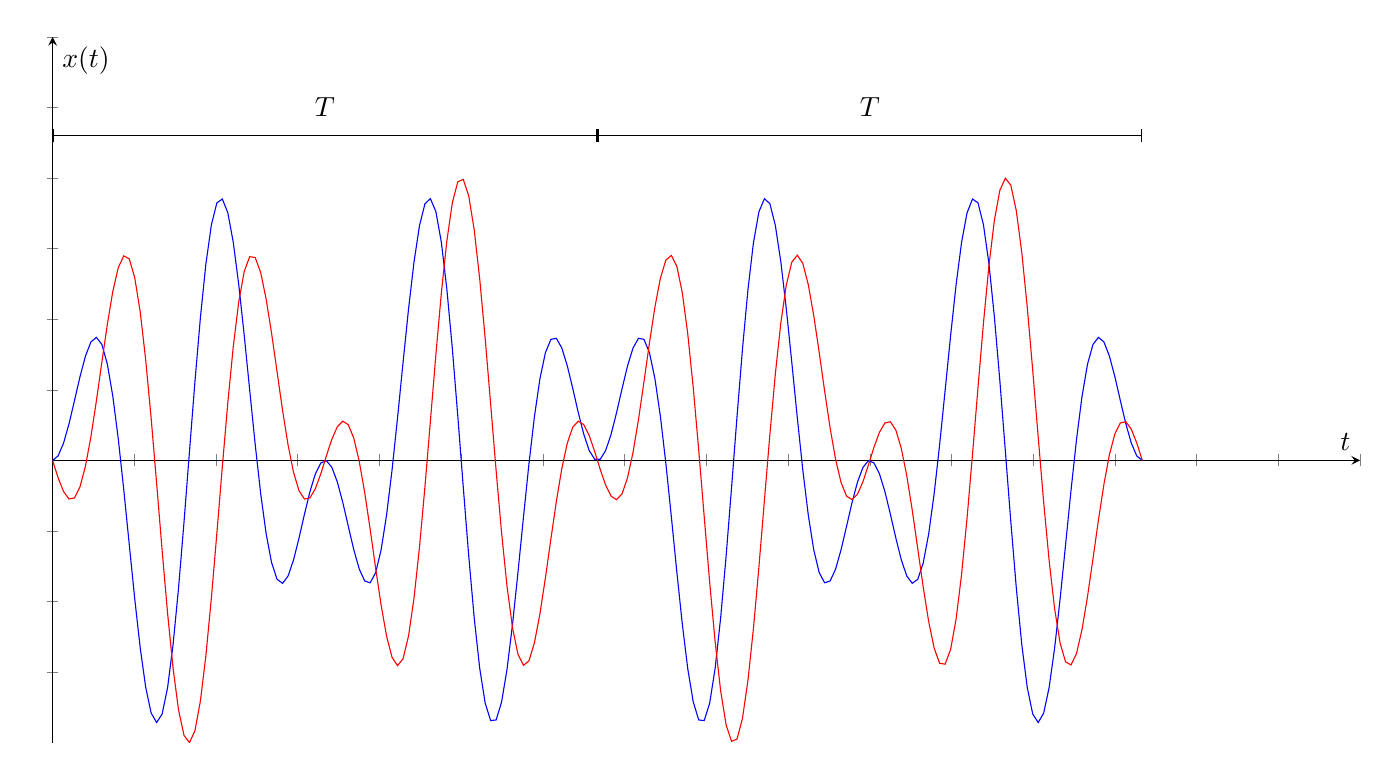
\begin{tikzpicture}
      % \begin{pgfinterruptboundingbox}
      \begin{axis}[width=1.5\textwidth, height=30em,
          %	title={Discrete-time signal},
          axis x line=center,
          axis y line=middle,
          xmax=0.8,
          xlabel=$t$,
          xticklabels={,,},
          yticklabels={,,},
          ymax=3.0,
          ylabel=$x(t)$]

        \addplot[domain=-0:0.666666667,samples=200,color=blue] {cos( deg(2*3.1415*9*x))-
          cos( deg(2*3.1415*15*x))};
        \addplot[domain=-0:0.666666667,samples=200,color=red] {sin( deg(2*3.1415*9*x))-
          sin( deg(2*3.1415*15*x))};

        \node at (axis cs:0.16666667,2.5) {$\displaystyle{T}$};
        \addplot [dimen] plot coordinates {(0,2.3) (0.33333,2.3)};
        \node at (axis cs:0.33333333+0.16666667,2.5) {$\displaystyle{T}$};
        \addplot [dimen] plot coordinates {(0.33333,2.3) (0.6666667,2.3)};

      \end{axis}
      %\end{pgfinterruptboundingbox}
      %\draw[use as bounding box] ([xshift=0cm,yshift=0cm]current axis.south west) 
      %    rectangle ([xshift=0cm,yshift=0cm]current axis.north east);
    \end{tikzpicture}
  \end{center}
  \caption{Periodic function $e^{i 2\pi 9t} - e^{i 2\pi 15t}$. 
  Blue denotes the real and red denotes the imaginary component of the signal.}
  \label{fig:ex_periodic}
\end{marginfigure}

A consequence of Equation \ref{eq:integer_multiple} is that the ratios
of all pairs of angular frequencies $\omega_k$ and $\omega_{\ell}$ in
Equation \ref{eq:general_spectrum} need to be rational numbers. In
other words, it must be possible to express them in the following form
\begin{equation}
  \frac{\omega_k}{\omega_{\ell}} = \frac{n}{m} \in \mathbb{Q} \,\,
\end{equation}
in order for the signal to be periodic. Here $n$ and $m$ are arbitrary
integers and $k$ and $\ell$ are all unique combinations of the
frequency indices.  If the ratio of two real numbers
$\omega_1,\omega_2\in\mathbb{R}$ is a rational number
$\omega_1/\omega_2 \in \mathbb{Q}$, the numbers $\omega_1$ and
$\omega_2$ are called \emph{\index{commensurable}{commensurable}.}
All angular frequencies for a Fourier series need to be commensurable
relative to one another in order for the signal to be periodic.

How does one determine the fundamental frequency $\omega$? It is
possible to apply \emph{\index{Euclid's algorithm}{Euclid's
algorithm}}. This is sometimes referred to as
the \emph{\index{greatest common divisor}{greatest common divisor}}
for the set of frequencies $\omega_k$. Note that this algorithm will
only produce a result in a finite number of steps if the set of
numbers $\{\omega_k\}$ are commensurable!

\newthought{Here is an example}. Let us assume that a signal is defined as
\begin{equation}
  x(t) = c_1 e^{i \omega_1 t} + c_2 e^{i \omega_2 t} = e^{i 2\pi 9t} -
  e^{i 2\pi 15t} \,\,.
\end{equation}
Is this signal periodic? If so, what is its fundamental frequency
$\omega$ and fundamental period $T$?

In order for this signal to be periodic, $\omega_1$ and $\omega_2$
must be commensurable.  In other words,
$\omega_1/\omega_2 \in \mathbb{Q}$. This is the case, as it is clear
that $\omega_1/\omega_2 = 3/5$ is a rational number.

This signal has two unique angular frequencies: $\omega_1 = 2\pi 9$
and $\omega_2 = 2\pi 15$.  Let's use Euclid's algorithm\sidenote{The
general principle behind the algorithm is that if $\omega_1
= \omega \ell_1$ and $\omega_2=\omega \ell_2$ with $\ell_1$ and
$\ell_2$ integers, then $\omega_1 - \omega_2 = \omega(\ell_1-\ell_2)$
is still divisible with $\omega$.} on these two numbers to determine
the fundamental angular frequency $\omega$.  We start with the two
numbers: $(2\pi 9, 2\pi15)$. Then subtract the smallest number from
the largest number $2\pi 15 - 2\pi 9 = 2\pi 6$ and replace the larger
number with the remainder: $(2\pi 9, 2\pi 6)$.  We repeat this process
until both numbers are the same.  All the iterations are shown below:
\begin{align*}
  (2\pi 15, 2\pi 9)        &                     \\
  (2\pi 15-2\pi 9, 2\pi 9) & = (2\pi 6, 2\pi 9)  \\
  (2\pi 6, 2\pi 9-2\pi 6)  & = (2\pi 6, 2\pi 3)  \\
  (2\pi 6-2\pi 3, 2\pi 3)  & = (2\pi 3, 2\pi 3).
\end{align*}
And we thus find that the fundamental frequency is $\omega=2\pi 3$ and, using
Equation \ref{eq:fundamental_period}, we find that $T = 1/3$.

\begin{marginfigure}[1cm]
  \begin{center}
    \includegraphics[width=\textwidth]{ch01/figures/fourier_head.jpg}
  \end{center}
  \caption{Jean-Baptiste Joseph Fourier}
  \label{fig:joe_fourier2}
\end{marginfigure}

\newthought{The Fourier series is a spectral representation of a periodic function} and is defined as
\begin{equation}
  \boxed{
    x_N(t) = \sum_{k=-N}^{N} c_k e^{i \frac{2\pi}{T} k t}
    \label{eq:synthesis_eq}
  } \,\,.
\end{equation}
The fundamental period of a periodic signal is related to the fundamental angular frequency
as follows: $T=2\pi/\omega$.
We can turn this around and express the fundamental angular frequency as a function of
the fundamental period $\omega=2\pi/T$, as we have done above.


This Fourier series is named after Jean-Baptiste Joseph Fourier
(1768–1830).  He introduced this representation for the purpose of
solving the heat equation using a series of sinusoidal characteristic
solutions. Perhaps the most revolutionary outcome of his study was
that a wide range of functions can be represented as a sum of
elementary sinusoidal functions.

Given a set of Fourier series coefficients $c_k$, we can synthesize a
signal $x_N(t)$.  This procedure is
called \emph{\index{synthesis}{synthesis}}.  This formula shown in
Equation \ref{eq:synthesis_eq} is also called the Fourier series
synthesis equation.\sidenote{Synthesis: \begin{equation*}c_{-N},c_{-N+1},\cdots,c_{N} \rightarrow x_N(t)\end{equation*}\\Analysis: \begin{equation*}x(t) \rightarrow c_{-N},c_{-N+1},\cdots,c_{N}\end{equation*}}

The inverse operation, determining coefficients $c_k \in \mathbb{C}$ from a certain
periodic signal $x(t)$, is called \emph{\index{analysis}{analysis}}.
We'll slowly work our way to this formula.

We will not study the convergence of the Fourier series, which means investigating
if $\lim_{N\rightarrow \infty} x_N(t) = x(t)$. This is outside the scope of this course.

\newthought{In order to find the analysis formula, we'll first need to introduce the concept of
  basis functions and an inner product}. A Fourier series basis function is defined
as $\psi_k(t)=e^{i\frac{2\pi}{T} k t}$.
We can use this to write the Fourier series in the following form:
\begin{equation}
  x_N(t) = \sum_{k=-N}^{N} c_k e^{i \frac{2\pi}{T} k t} = \sum_{k=-N}^{N} c_k \psi_k(t) \,\,.
\end{equation}
The terms $\psi_k(t)$ can be seen as a set of orthogonal basis
functions for a periodic function with a period $T$. What does it mean
that basis functions $\psi_k(t)$ are orthogonal?  We'll first need to
define an inner product.


%The set of basis function
%$\{\psi_k(t)\}_{k=-\infty}^{\infty}$ forms a vector space.\footnote{In mathematics, we would talk about a Hilbert space
%in this context. We have tried to avoid going into too much detail about
%this topic here.}


%\sidenote{If you are familiar with what a Hilbert space is, then you'll recognize this. Don't worry if you've never even heard of a Hilbert space though.}

For periodic functions $a(t)$ and $b(t)$ with period $T$, an inner product is defined as:
\begin{equation}
  \langle a(t), b(t) \rangle = \int_{t_0}^{t_0+T} a(t) b^*(t) dt = \int_T a(t) b^*(t) dt \,\,,
  \label{eq:inner_product_def}
\end{equation}
where $t_0$ is an arbitrary value of time, and $T$ is the fundamental period of the signal.
Because of the periodicity of the signals, we can evaluate the integral at any offset $t_0$ we wish to.
The right-hand side is just an alternative way to denote the equation in the middle, i.e.,
that we integrate over one period of the periodic function.

When taking the inner product between two basis functions, we obtain:
\begin{align}
  \langle \psi_\ell(t), \psi_k(t) \rangle & = \int_T \psi_\ell(t) \psi_k^*(t) dt            \\
                                          & = \int_T e^{i\frac{2\pi}{T}(\ell-k) t} dt \,\,.
\end{align}
Let's break this down into two cases. First let's look at $\ell=k$. 
We know that $e^{i(2\pi t/T)(\ell-\ell)}=e^{i \cdot 0} = 1$. It is easy to see that:
\begin{align}
  \langle \psi_\ell(t), \psi_\ell(t) \rangle & = \int_{0}^T dt \\
                                             & = T \,\,.
\end{align}
I've arbitrarily chosen to use $t_0=0$ when evaluating the integral (see the definition of the
inner product in Equation \ref{eq:inner_product_def}). I would have obtained the same result with any value of $t_0$.

Let's look at the other case where $\ell \ne k$. This means that the frequencies of the complex
sinusoidal signals are different. We know that $\ell - k$ is a non-zero integer.
Evaluating the inner product in this case gives us:
\begin{align}
  \langle \psi_\ell(t), \psi_k(t) \rangle & = \int_0^T  e^{i\frac{2\pi}{T}t(\ell-k)} dt                                                           \\
                                          & = \left.\frac{T}{2\pi i (\ell-k)} e^{i\frac{2\pi}{T}t(\ell-k)} \right\vert_{t=0}^{T}                  \\
                                          & = \frac{T}{2\pi i (\ell-k)}\left( e^{i\frac{2\pi}{T}T(\ell-k)} - e^{i\frac{2\pi}{T}0(\ell-k)} \right) \\
                                          & = \frac{T}{2\pi i (\ell-k)}( 1 - 1 )                                                                  \\
                                          & = 0 \,\,.
\end{align}
We can combine these two results conveniently as:
\begin{align}
  \langle \psi_\ell(t), \psi_k(t) \rangle = T\delta_{\ell,k} \,\,.
\end{align}
The integral thus evaluates to $T$ when $\ell=k$ and zero
otherwise. We have used the Kronecker delta function $\delta_{k,\ell}$
for convenience. It is defined as:
\begin{equation}
  \delta_{k,\ell} = \left\{
  \begin{array}{rcr}
    1 & \mathrm{when} & \ell=k     \\
    0 & \mathrm{when} & \ell \ne k \\
  \end{array}\right.\,\,.
  %\right\} 
\end{equation}
This is the definition of \emph{\index{orthogonality of basis
functions}{orthogonality of basis functions}}. We now have what we
need to introduce the analysis formula, which relies on orthogonality.

\newthought{The Fourier series analysis formula is defined as}:
\begin{equation}
  \boxed{
    c_k = \frac{1}{T}\langle x(t), \psi_k(t) \rangle = \frac{1}{T}\int_T x(t) \psi_k^*(t) dt = \frac{1}{T}\int_T x(t) e^{-i \frac{2\pi}{T} k t} dt
  } \,\,.
\end{equation}
This formula can be used to determine what the Fourier series coefficients are for a
periodic function $x(t)$. The proof for the analysis formula relies on the orthogonality
of basis functions. We'll make the assumption that there exists a Fourier series representation
for the signal $x(t)$ in the form of an infinite sum and that this sum
converges uniformly\sidenote{The mathematician A.N. Kolmogorov pointed out in his 1923
  paper several examples of functions for which the Fourier series diverges.
  The topic Fourier series convergence is beyond the scope of this course. \cite{kolmogoroff1923serie}}:
\begin{equation}
  x(t) = \sum_{\ell=-\infty}^{\infty} c_{\ell} e^{i\frac{2\pi}{T}\ell t} \,\,.
\end{equation}
If this is the case, then the inner product, i.e., the analysis
equation, has the following result:
\begin{align}
  \frac{1}{T}\langle x(t), \psi_k(t) \rangle & = \frac{1}{T}\int_T \left(\sum_{\ell=-\infty}^{\infty} c_\ell e^{i\frac{2\pi}{T}\ell t}\right) e^{-i\frac{2\pi}{T}k t}dt \\
                                             & =\frac{1}{T}\sum_{\ell=-\infty}^{\infty} \int_T c_{\ell} e^{i\frac{2\pi}{T}\ell t} e^{-i\frac{2\pi}{T}kt}dt              \\
                                             & = \frac{1}{T}\sum_{\ell=-\infty}^{\infty}c_{\ell} \int_T e^{i\frac{2\pi}{T}(\ell-k)t}dt                                  \\
                                             & = \frac{1}{T}\sum_{\ell=-\infty}^{\infty}c_{\ell} T \delta_{\ell,k}                                                      \\
                                             & = c_k \,\,.
\end{align}
This proves that we can go back and forth between the Fourier synthesis and analysis formula,
as long as there exists a Fourier series representation that 
converges uniformly for the periodic signal $x(t)$.

\newthought{We now have the synthesis and analysis formulas for a Fourier series}.
The synthesis formula allows us to obtain the time domain representation of a 
periodic signal using Fourier coefficients:
\begin{equation}
  \boxed{
    x_N(t) = \sum_{k=-N}^{N} c_k e^{i \frac{2\pi}{T}kt}
  } \,\,.
\end{equation}
The inverse operation, i.e., obtaining the Fourier coefficients $c_k$ from a
periodic function $x(t)$, is as follows:
\begin{equation}
  \boxed{
    c_k = \frac{1}{T} \int_T x(t) e^{-i \frac{2\pi}{T}kt} dt
  } \,\,.
\end{equation}

\newthought{What about real-valued signals?} We can use Euler's formula to look at
the real part of the Fourier series synthesis formula. I'll assume again that $x(t)$ is a
periodic function that can be represented using an infinite sum of complex sinusoidal signals:
\begin{equation}
  x(t) = \sum_{\ell = -\infty}^{\infty} c_{\ell} e^{i\frac{2\pi}{T}\ell t}.
\end{equation}
The real part of the signal $x(t)$ is:
\begin{align}
  \mathrm{Re}\{x(t)\} & = \frac{1}{2} (x(t) + x^*(t))                                                                                                                                             \\
                      & = \frac{1}{2}\sum_{\ell=-\infty}^{\infty} c_{\ell} e^{i\frac{2\pi}{T}\ell t} + \frac{1}{2}\sum_{\ell=-\infty}^{\infty} c^*_{\ell} e^{-i\frac{2\pi}{T}\ell t}              \\
                      & = \frac{1}{2}(c_0 + c_0^*) + \frac{1}{2}\sum_{\ell=1}^{\infty}[ (c_{\ell} + c^*_{-\ell}) e^{i\frac{2\pi}{T}\ell t} + (c^*_{\ell} + c_{-\ell}) e^{-i\frac{2\pi}{T}\ell t}] \\
                      & = A_0 + \sum_{\ell=1}^{\infty} A_\ell \cos\left(\frac{2\pi}{T}\ell t+\phi_\ell\right) \,\,.
  \label{eq:real_fourier_series}
\end{align}
For the last part, I've introduced new variables: $A_0= \frac{1}{2}(c_0 + c_0^*) \in \mathbb{R}$, $A_\ell = |c_{\ell} +c^*_{-\ell}|\in \mathbb{R}_{\ge 0}$ and $\phi_\ell = \angle (c_{\ell} + c^*_{-\ell}) \in \mathbb{R}$.

When analyzing Fourier series coefficients for a real-valued function,
you will find that they come in conjugate symmetric pairs, which will
allow you to write the Fourier series synthesis equation in the form
shown on the last line of Equation \ref{eq:real_fourier_series}.  The
Fourier series synthesis equation is sometimes introduced in this
form. But this only applies to real valued signals!

\newthought{The zero frequency or the direct current (DC) frequency component $c_0$} often has a
special meaning. In the case of real-valued signals, this is the only
frequency component that does not have a positive and negative
frequency conjugate symmetric pairing. The DC component also has the
meaning that it is the mean value of the signal:
\begin{equation}
  c_0 = \frac{1}{T} \int_{T} x(t) dt \,\,.
\end{equation}

\newthought{A partial sum Fourier series can be used to approximate a periodic signal}.
This is especially useful, if one knows that the signal is band-limited,
and one knows \emph{a priori} that higher order terms (high frequency components)
are not present in the signal, or they have such low magnitudes that they are not significant.

A partial sum synthesis formula only uses a subset of the Fourier coefficients:
\begin{equation}
  x_S(t) = \sum_{k \in S} c_k e^{i 2\pi kt/T} \,\,,
\end{equation}
where $S$ is a set of Fourier series coefficient indices.

\begin{marginfigure}
  \begin{center}
    \begin{tikzpicture}
      \pgfmathdeclarefunction{p}{1}{%
        \pgfmathparse{(and(mod(#1,2)>0, mod(#1,2)<1))}%
      } \begin{axis}[
          width=7cm,
          axis lines = center,
          ymax=1.5,
          ymin=0,
          xmax=3.5,
          xmin=-3.5,
          legend pos=outer north east,
          yticklabels={,,},
          xticklabels={,,},
          xlabel={$t$},
          ylabel={$x(t)$}
        ]

        \addplot+[ycomb,color=blue,mark=triangle*,mark options={blue}] plot coordinates {
            (-3,1)
            (-2,1)
            (-1,1)
            (-0,1)
            (1,1)
            (2,1)
            (3,1)
          };

        \node at (axis cs:1.5,1.15) {$\displaystyle{T}$};
        \addplot [dimen] plot coordinates {(1,1.1) (2,1.1)};

      \end{axis}
    \end{tikzpicture}
  \end{center}
  \caption{The Dirac comb signal, an infinitely long train of unit impulses spaced apart by $T$. The Dirac comb is a periodic function with a fundamental period $T$.
    The Dirac comb is used to model sampling values of a continuous-time signal spaced evenly apart to provide an idealized model for discretizing a continuous-time signal.}
  \label{fig:dirac_comb_plot2}
\end{marginfigure}

A partial sum approximation of this type is often used in audio, image, and video compression,
which rely on storing only a small subset of Fourier series coefficients, which typically have
the largest magnitudes, leaving out the frequency components with small magnitudes.

\newthought{Example: Let's represent the so-called Dirac comb using a Fourier series}.
The Dirac comb is a signal that consists of a train of unit impulse functions spaced $T$ apart from one another.
It is defined as:
\begin{equation}
  x(t) = \sum_{k=-\infty}^{\infty} \delta(t - k T) \,\,.
\end{equation}
This signal is shown in Figure \ref{fig:dirac_comb_plot2}. We'll encounter this signal when introducing
the model for discretizing a continuous-time signal.

The fundamental period for this signal is $T$. Therefore, one would expect that we can form a Fourier
series representation of this signal. What are the values of the coefficients $c_k$? Let's find out using the analysis formula.

We'll evaluate the analysis integral formula from $t=-T/2$ to $t=T/2$, as this is convenient in the case of this signal.
The analysis formula evaluates to:
\begin{align}
  c_k & = \langle x(t),\psi_k(t) \rangle = \frac{1}{T} \int_{-T/2}^{T/2} \delta(t) e^{-i\frac{2\pi}{T}kt} dt \\
      & = \frac{1}{T}\label{eq:dirac_comb_coeff} \,\,.
\end{align}
The signal can thus be represented as the following Fourier series:
\begin{equation}
  x_N(t) = \frac{1}{T}\sum_{k=-N}^{N} e^{i\frac{2\pi}{T}kt} \,\,.
\end{equation}
Take a look at Figure \ref{fig:fs_fig0}. This is an approximation of the Dirac comb $x_7(t)$ using 15 frequency components.
I hope it is not too difficult for you to convince yourself that as we increase the value of $N$,
the spikes will become sharper and sharper.

\begin{marginfigure}[-8cm]
  \begin{center}
    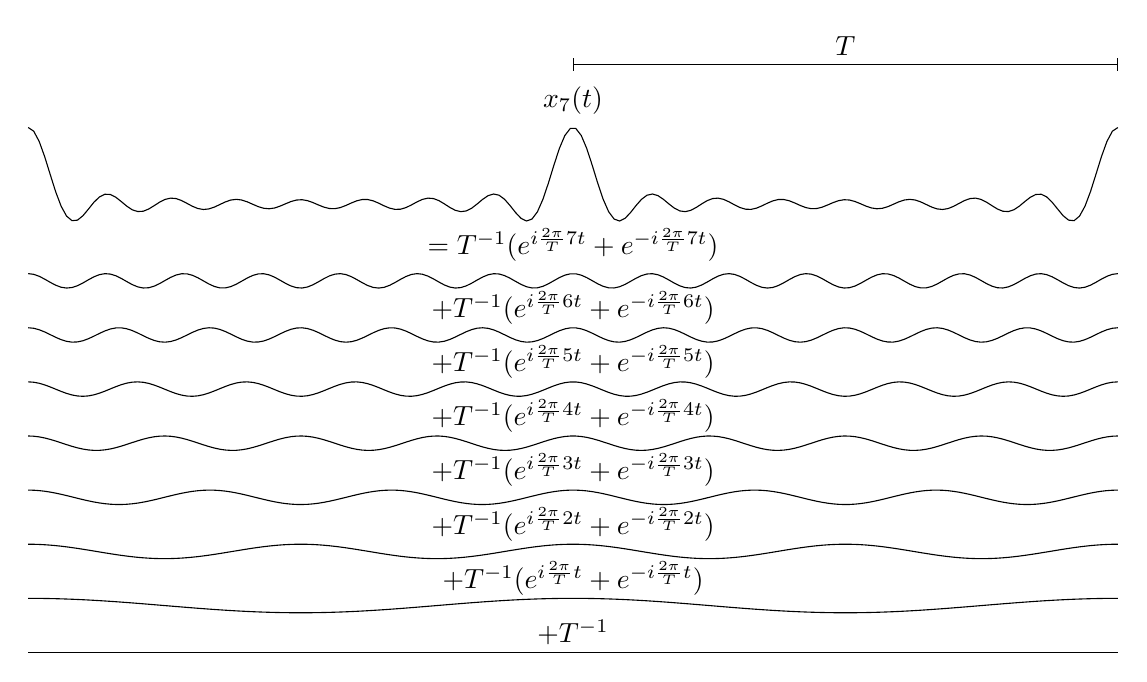
\begin{tikzpicture}
      % \begin{pgfinterruptboundingbox}
      \begin{axis}[width=1.5\textwidth, height=30em,
          %	title={Discrete-time signal},
          axis x line=none,
          axis y line=none
        ]
        \addplot[domain=-100:100,samples=200] {27+
          cos( deg(2*3.1415*0.01*x))+
          cos( deg(2*3.1415*0.01*2*x) )+
          cos( deg(2*3.1415*0.01*3*x) )+
          cos( deg(2*3.1415*0.01*4*x) )+
          cos( deg(2*3.1415*0.01*5*x) )+
          cos( deg(2*3.1415*0.01*6*x) )+
          cos( deg(2*3.1415*0.01*7*x) )+
          cos( deg(2*3.1415*0.01*8*x) ) };

        \node at (axis cs:50.0,44) {$\displaystyle{T}$};
        \addplot [dimen] plot coordinates {(0,42) (100,42)};

        \node at (axis cs:0,38) {$x_{7}(t)$};

        \node at (axis cs:0,22) {$= T^{-1} (e^{i\frac{2\pi }{T}7t} + e^{-i\frac{2\pi }{T}7t})$};
        \node at (axis cs:0,15) {$+ T^{-1} (e^{i\frac{2\pi }{T}6t} + e^{-i\frac{2\pi }{T}6t})$};
        \node at (axis cs:0,9) {$+ T^{-1}(e^{i\frac{2\pi }{T}5t} + e^{-i\frac{2\pi }{T}5t})$};
        \node at (axis cs:0,3) {$+ T^{-1}(e^{i\frac{2\pi }{T}4t} + e^{-i\frac{2\pi }{T}4t})$};
        \node at (axis cs:0,-3) {$+ T^{-1}(e^{i\frac{2\pi }{T}3t} + e^{-i\frac{2\pi }{T}3t})$};
        \node at (axis cs:0,-9) {$+ T^{-1}(e^{i\frac{2\pi }{T}2t} + e^{-i\frac{2\pi }{T}2t})$};
        \node at (axis cs:0,-15) {$+ T^{-1}(e^{i\frac{2\pi }{T}t} + e^{-i\frac{2\pi }{T}t})$};
        \node at (axis cs:0,-21) {$+ T^{-1}$};

        \addplot[domain=-100:100,samples=200] {-24+0.8*cos( deg(2*3.1415*0.0*x) ) };
        \addplot[domain=-100:100,samples=200] {-18+0.8*cos( deg(2*3.1415*0.01*x) ) };
        \addplot[domain=-100:100,samples=200] {-12+0.8*cos( deg(2*3.1415*0.01*2*x) ) };
        \addplot[domain=-100:100,samples=200] {-6+0.8*cos( deg(2*3.1415*0.01*3*x) ) };
        \addplot[domain=-100:100,samples=200] {0+0.8*cos( deg(2*3.1415*0.01*4*x) ) };
        \addplot[domain=-100:100,samples=200] {6+0.8*cos( deg(2*3.1415*0.01*5*x) ) };
        \addplot[domain=-100:100,samples=200] {12+0.8*cos( deg(2*3.1415*0.01*6*x) ) };
        \addplot[domain=-100:100,samples=200] {18+0.8*cos( deg(2*3.1415*0.01*7*x) ) };

      \end{axis}
      %\end{pgfinterruptboundingbox}
      %\draw[use as bounding box] ([xshift=0cm,yshift=0cm]current axis.south west) 
      %    rectangle ([xshift=0cm,yshift=0cm]current axis.north east);
    \end{tikzpicture}
  \end{center}
  \caption{A Fourier series representation $x_{7}(t)=\frac{1}{T}\sum_{k=-7}^{7} e^{i\frac{2\pi}{T}k t}$ of a Dirac comb signal $x(t)=\sum_{k=-\infty}^{\infty}\delta(t-k T)$
    with a period $T$. Two periods of the signal are shown. The Fourier series representation of the signal is made using seven sinusoidal signals.}
  \label{fig:fs_fig0}
\end{marginfigure}

You should also be able to convince yourself that this signal is
real-valued, by investigating the pairing of positive and negative
frequency terms:
\begin{align}
  x_N(t) & = \frac{1}{T}\sum_{k=-N}^{N} e^{i\frac{2\pi}{T}kt}                                        \\
         & = \frac{1}{T} + \frac{1}{T} \sum_{k=1}^{N} (e^{i\frac{2\pi}{T}kt}+e^{-i\frac{2\pi}{T}kt}) \\
         & = \frac{1}{T} + \frac{2}{T} \sum_{k=1}^{N} \cos\left( \frac{2\pi}{T}kt \right ) \,\,.
\end{align}
This is how the positive and negative frequency terms are organized in Figure \ref{fig:fs_fig0}.
For real-valued Fourier series representations, this sort of grouping of positive and negative
frequency coefficients always occurs.


\newthought{Example: Fourier series representation for a square wave}. A square wave is a
classic example of a periodic function that can be evaluated using a Fourier series. This type of signal
is often used, e.g., in the pulse width modulation scheme of adjusting mean power flowing through a circuit.
This type of on-off pulsing scheme is also used in avalanche rescue beacons used to radiolocate
victims buried under snow. The rectangular function is shown in Figure \ref{fig:square_wave_example}.
A measurement of power emitted by an avalanche rescue beacon as a function of time is shown in Figure \ref{fig:avibeacon}.

\begin{marginfigure}
  \begin{center}
    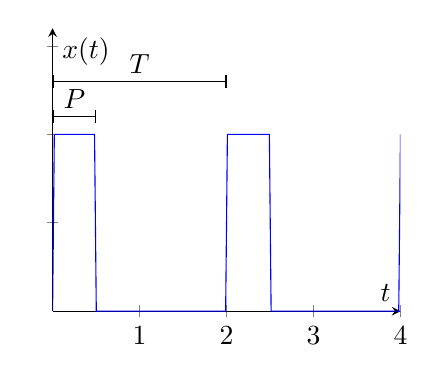
\begin{tikzpicture}
      \pgfmathdeclarefunction{p}{1}{%
        \pgfmathparse{(and(mod(#1,2)<0.5,and(mod(#1,2)>0, mod(#1,2)<1)))}%
      }
      \begin{axis}[
          width=6cm,
          domain=0:(4),
          samples=200,
          axis lines =center,
          ymax=1.6,
          yticklabels={,,},
          legend pos=outer north east ,xlabel={$t$},ylabel={$x(t)$}]
        \addplot[blue] {p(x)};

        \node at (axis cs:0.25,1.2) {$\displaystyle{P}$};
        \addplot [dimen] plot coordinates {(0,1.1) (0.5,1.1)};

        \node at (axis cs:1,1.4) {$\displaystyle{T}$};
        \addplot [dimen] plot coordinates {(0,1.3) (2,1.3)};


        %    \legend{$\mathrm{Re}(e^{j2t})$,$\mathrm{Im}(e^{j2t})$}
      \end{axis}
    \end{tikzpicture}
  \end{center}
  \caption{A classic example of a commonly encountered periodic function, 
  the square wave signal. This type of signal is encountered, e.g., with pulse width modulation in electrical engineering.}
  \label{fig:square_wave_example}
\end{marginfigure}


\begin{marginfigure}
  \begin{center}
    \includegraphics[width=\textwidth]{ch07/figures/avibeacon.png}
  \end{center}
  \caption{A measurement of power as a function of time transmitted by an avalanche rescue locator beacon. Approximately a 0.1 second pulse is emitted every second.}
  \label{fig:avibeacon}
\end{marginfigure}

Consider a general square wave signal with period $T$, pulse length $P$ and amplitude $1$. Between $0\le t < T$,
this signal is mathematically described with:
\begin{equation}
  x(t) = \left\{ \begin{array}{ccl}
    1 & \mathrm{when}      & 0 \le t < P \\
    0 & \mathrm{otherwise} &
  \end{array}
  \right. \,\,.
\end{equation}
By analytically evaluating the Fourier series analysis integral one has:
\begin{equation}
  c_k = \frac{1}{T}\int_0^T x(t) e^{-i 2\pi k t/T} dt \,\,,
\end{equation}
we can obtain an equation for coefficients $c_k$. In the case of $k=0$, the integral evaluates to:
\begin{align}
  c_0 & = \frac{1}{T}\int_0^{T} x(t) e^{i\cdot 0}dt \\
      & = \frac{1}{T}\int_0^{P}  dt                 \\
      & = \frac{P}{T} \,\,.\label{eq:pulsecoeff0}
\end{align}
For other values of $k\ne 0$:
\begin{align}
  c_k & = \frac{1}{T}\int_0^{T} x(t) e^{-i\frac{2\pi}{T} t k}dt                                                   \\
      & =  \frac{1}{T}\int_0^{P}  e^{-i\frac{2\pi}{T} t k}dt                                                      \\
      & = \left.-\frac{1 }{2i \pi k}e^{-i\frac{2\pi}{T}  t k}\right\vert_{t=0}^{P}                                \\
      & = -\frac{1}{2i\pi k}\left(e^{-i\frac{2\pi}{T}  k P} - 1\right)                                            \\
      & = \frac{1}{2i\pi k}e^{-i\frac{\pi}{T}  k P}\left(e^{i \frac{\pi}{T} kP} - e^{-i \frac{\pi}{T} kP} \right) \\
      & =  \frac{1}{\pi k}e^{-i\frac{\pi}{T}  k P}\sin\left(\frac{\pi}{T} kP\right) \,\,.\label{eq:pulsecoeff1}
\end{align}
We have used: the inverse Euler's formula for the $\sin(\cdot)$ signal, the fact
that $e^{-i\frac{\pi}{T} k P}e^{i\frac{\pi}{T} k P}=1$, and that $\sin(-\theta)=-\sin(\theta)$.

\begin{marginfigure}
  \begin{center}
    \includegraphics[width=\textwidth]{code/009_square_wave/square_wave.png}
  \end{center}
  \caption{Fourier series approximation of a square wave evaluated with the Python script \texttt{009\_square\_wave/square\_wave.py}.}
  \label{fig:square_wave_python}
\end{marginfigure}

Now we can evaluate the synthesis formula to form a Fourier series approximation of this function:
\begin{align}
  x_N(t) & = c_0 + \sum_{k=1}^{N} c_k e^{i\frac{2\pi}{T}kt} + c_{-k} e^{-i\frac{2\pi}{T}kt}                                                                                                     \\
         & = \frac{P}{T} + \sum_{k=1}^{N} \frac{\sin\left(\frac{\pi}{T} kP\right)}{\pi k}  \left(e^{-i\frac{\pi}{T}kP}e^{i\frac{2\pi}{T}kt} + e^{i\frac{\pi}{T}kP}e^{-i\frac{2\pi}{T}kt}\right) \\
         & = \frac{P}{T} + \sum_{k=1}^{N} \frac{2\sin\left(\frac{\pi}{T} kP\right)}{\pi k} \cos\left( \frac{2\pi}{T}kt-\frac{\pi}{T}kP\right) \,\,.
\end{align}
Let's see what this function looks like. I've written a little Python
program to visualize the Fourier series approximation of this
function. The Python code is found in
Listing \ref{lst:fourier_square_code}. The output of this program is shown in Figure \ref{fig:square_wave_python}.

\lstinputlisting[language=Python, caption={\texttt{009\_square\_wave/square\_wave.py}}, label=lst:fourier_square_code]{code/009_square_wave/square_wave.py}

\if 0
  \begin{center}
    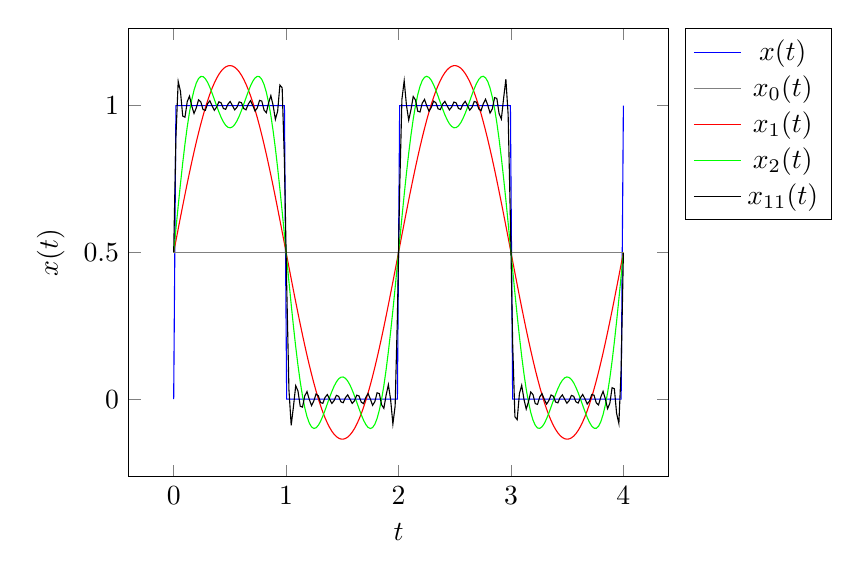
\begin{tikzpicture}
      \pgfmathdeclarefunction{p}{1}{%
        \pgfmathparse{(and(mod(#1,2)>0, mod(#1,2)<1))}%
      }
      \begin{axis}[domain=0:(4),samples=200, legend pos=outer north east ,xlabel={$t$},ylabel={$x(t)$}]
        \addplot[blue] {p(x)};
        \addplot[gray] {0.5}; % k=0
        \addplot[red] {0.5 + (2.0/3.1415)*cos(deg(3.1415*x - 1.571))}; % k=1
        \addplot[green] {0.5 + (2.0/3.1415)*cos(deg(3.1415*x - 1.571)) + (2.0/(3.1415*3))*cos(deg(3.1415*3*x - 1.571))}; % k=2
        %  \addplot[orange] {0.5 + (2.0/3.1415)*cos(deg(3.1415*x - 1.571)) + (2.0/(3.1415*3))*cos(deg(3.1415*3*x - 1.571)) + (2.0/(3.1415*5))*cos(deg(3.1415*5*x - 1.571))}; % k=5
        \addplot[black] {0.5 + (2.0/3.1415)*cos(deg(3.1415*x - 1.571))
          + (2.0/(3.1415*3))*cos(deg(3.1415*3*x - 1.571))
          + (2.0/(3.1415*5))*cos(deg(3.1415*5*x - 1.571))
          + (2.0/(3.1415*7))*cos(deg(3.1415*7*x - 1.571))
          + (2.0/(3.1415*9))*cos(deg(3.1415*9*x - 1.571))
          + (2.0/(3.1415*11))*cos(deg(3.1415*11*x - 1.571))
          + (2.0/(3.1415*13))*cos(deg(3.1415*13*x - 1.571))
          + (2.0/(3.1415*15))*cos(deg(3.1415*15*x - 1.571))
          + (2.0/(3.1415*17))*cos(deg(3.1415*17*x - 1.571))
          + (2.0/(3.1415*19))*cos(deg(3.1415*19*x - 1.571))
          + (2.0/(3.1415*21))*cos(deg(3.1415*21*x - 1.571))};
        %%                     + (2.0/(3.1415*23))*cos(deg(3.1415*23*x - 1.571))
        %                     + (2.0/(3.1415*25))*cos(deg(3.1415*25*x - 1.571))
        %                     + (2.0/(3.1415*27))*cos(deg(3.1415*27*x - 1.571))
        %                     + (2.0/(3.1415*29))*cos(deg(3.1415*29*x - 1.571))
        %                     + (2.0/(3.1415*31))*cos(deg(3.1415*31*x - 1.571))
        %                     + (2.0/(3.1415*33))*cos(deg(3.1415*33*x - 1.571))
        %                     + (2.0/(3.1415*35))*cos(deg(3.1415*35*x - 1.571))
        %                     + (2.0/(3.1415*37))*cos(deg(3.1415*37*x - 1.571)) 
        %                     + (2.0/(3.1415*39))*cos(deg(3.1415*39*x - 1.571)) 
        %                     + (2.0/(3.1415*41))*cos(deg(3.1415*41*x - 1.571)) 
        %                     + (2.0/(3.1415*43))*cos(deg(3.1415*43*x - 1.571)) 
        %                     + (2.0/(3.1415*45))*cos(deg(3.1415*45*x - 1.571)) 
        %                     + (2.0/(3.1415*47))*cos(deg(3.1415*47*x - 1.571)) 
        %                     + (2.0/(3.1415*49))*cos(deg(3.1415*49*x - 1.571)) 
        %                     + (2.0/(3.1415*51))*cos(deg(3.1415*51*x - 1.571)) 
        %                     + (2.0/(3.1415*53))*cos(deg(3.1415*53*x - 1.571)) 
        %                     + (2.0/(3.1415*55))*cos(deg(3.1415*55*x - 1.571))};

        \legend{$x(t)$,$x_0(t)$,$x_1(t)$,$x_2(t)$,$x_{11}(t)$}
      \end{axis}
    \end{tikzpicture}
  \end{center}
\fi

\newthought{The time derivative operator $\frac{d}{dt}$ has a very simple form for a Fourier series representation of a signal}.

We know that a Fourier series is a sum of complex sinusoidal signals. We also know that it is easy to differentiate this signal:
\begin{equation}
  \frac{d}{d t} c e^{i\omega t}=i\omega c e^{i\omega t}\,\,,
\end{equation}
where $c \in \mathbb{C}$ is a complex constant.

It is also relatively easy to see that the $n$th time derivative is:
\begin{equation}
  \frac{d^n}{dt^n}ce^{i\omega t} = (i\omega)^n c e^{i\omega t} \,\,.
\end{equation}
Thus, if $x(t)$ has a Fourier series representation
\begin{equation}
  x(t) = \sum_{k=-\infty}^{\infty} c_k e^{i\frac{2\pi}{T}kt}\,\,,
\end{equation}
then the $n$th time derivative has the following Fourier series representation:
\begin{align}
  \frac{d^n}{dt^n} x(t) & = \sum_{k=-\infty}^{\infty} i^n \left(\frac{2\pi k}{T}\right)^n c_k e^{i\frac{2\pi}{T}kt} \\
                        & = \sum_{k=-\infty}^{\infty} c^{(n)}_k e^{i\frac{2\pi}{T}kt} \,\,.
\end{align}
It is still a Fourier series, but with each Fourier coefficient modified in the following way:
\begin{equation}
  c_k^{(n)} := i^n \left(\frac{2\pi k}{T}\right)^n c_k \,\,.
  \label{eq:moddiff}
\end{equation}

Differentiation can be seen as a filtering operation on the signal. A filter is something
that modifies the amplitude and phase of the Fourier series coefficients in some way.
For example, a low-pass filtering operation would reduce the amplitudes of high frequency
coefficients relative to the amplitudes of the low frequency coefficients.
After a low-pass filtering operation, the ratio of low frequency coefficient amplitudes to
the high frequency coefficient amplitudes would be increased. A high pass filter on the other hand would do the opposite.

One thing to ask yourself is how does differentiation adjust the amplitude of each Fourier coefficient?
When taking the $n$th time derivative, what happens to the complex amplitudes at low angular
frequencies ($|2\pi k/T| < 1$)? What about high angular frequencies ($|2\pi k/T| > 1$)?
Hint, inspect how the coefficients defined in Equation \ref{eq:moddiff} are scaled.

The answer is that the magnitude of the low frequency Fourier coefficients are attenuated, and
high frequency ones are amplified. The DC component is completely removed as $2\pi k/T = 0$ for $k=0$.
Differentiation can therefore be viewed as a \emph{high-pass filtering} operation.

\newthought{The time shift operation $x(t-\tau)$ applied to a Fourier series representation} is also pretty handy.
Let's recall how a time shift affects a complex sinusoidal signal:
\begin{equation}
  x(t) = c e^{i\omega t} \,\,.
\end{equation}
If we apply a delay by $\tau$ to this signal $y(t) = x(t-\tau)$, we obtain:
\begin{align}
  y(t)  = c e^{i\omega (t-\tau)} =  e^{-i\omega \tau} c e^{i\omega t} = e^{-i\omega \tau} x(t) \,\,.
\end{align}
This means that a time delay by $\tau$ corresponds to a phase shift by $-\omega\tau$ for a complex sinusoidal signal.
We can apply this to a Fourier series, which is a sum of complex sinusoidal signals.

If the Fourier series representation of a signal is:
\begin{equation}
  x(t) = \sum_{k=-\infty}^{\infty} c_k e^{i\frac{2\pi}{T}kt} \,\,,
\end{equation}
then the Fourier series representation of a time shifted signal is:
\begin{align}
  x(t-\tau) & = \sum_{k=-\infty}^{\infty} \left(c_k e^{-i \frac{2\pi \tau}{T} k}\right) e^{i\frac{2\pi}{T}kt}\label{eq:time_shift_phasor} \\
            & =  \sum_{k=-\infty}^{\infty} c'_k e^{i\frac{2\pi}{T}kt}
\end{align}
where $c'_k$ is rotated on the complex plane in the clockwise direction by an angle of $2\pi k\tau/T$ with respect to $c_k$.

This means that if you know the Fourier series representation of a signal, you can easily modify the
complex amplitude $c_k$ of each Fourier coefficient to obtain the coefficients of the time shifted signal.

\newthought{What if a signal is not periodic, can we still form a spectral representation for a signal?}
Yes, we can. This investigation leads to the \emph{\index{continuous-time Fourier transform}{continuous-time Fourier transform}}.

Let's derive the continuous-time Fourier transform from the Fourier series. Pretty much all we'll need to do is
to study what happens when the fundamental period of the signal approaches infinity: $T\rightarrow \infty$.
We'll arrive with the result that introduces the Fourier transform, and the inverse Fourier transform, 
introducing, for the first time, this general spectral representation for continuous-time signals.

We start the derivation of the continuous-time Fourier transform with the definition of a Fourier series for a
function with period $T$. We'll denote by $\Delta \omega$ the spacing between frequency components.
The term $\Delta \omega$ also denotes the fundamental angular frequency of the periodic signal:
\begin{align}
  x_{T}(t) & = \sum_{k=-\infty}^{\infty} c_k e^{ik\Delta \omega t}  \,\,.
\end{align}
We can now add the definition of $c_k$ corresponding to the $k$th Fourier series coefficient using the synthesis equation:
\begin{align}
  x_{T}(t) & = \sum_{k=-\infty}^{\infty} \left[\frac{1}{T}\int_{-T/2}^{T/2} x_{T}(t) e^{-ik\Delta \omega t} dt\right]  e^{ik\Delta \omega t}  \,\,.
\end{align}
We then note that $1/T = \Delta \omega/2\pi$. This is the relationship between the fundamental period of
the signal and the fundamental angular frequency that we discussed in the beginning of this chapter.

We now obtain:
\begin{align}
  x_{T}(t) & = \frac{1}{2\pi}\sum_{k=-\infty}^{\infty} \left[\int_{-T/2}^{T/2} x_{T}(t) e^{-ik\Delta \omega t} dt\right]  e^{ik\Delta \omega t} \Delta \omega \\
           & = \frac{1}{2\pi}\sum_{k=-\infty}^{\infty} \hat{x}_{T}(k\Delta\omega)  e^{ik\Delta \omega t} \Delta \omega \,\,.
\end{align}
In this form, the equation is a Riemann sum approximation of an integral of a continuous function $\hat{x}_{T}(\omega)e^{-i\omega t}$.
\begin{figure}
  \begin{center}
    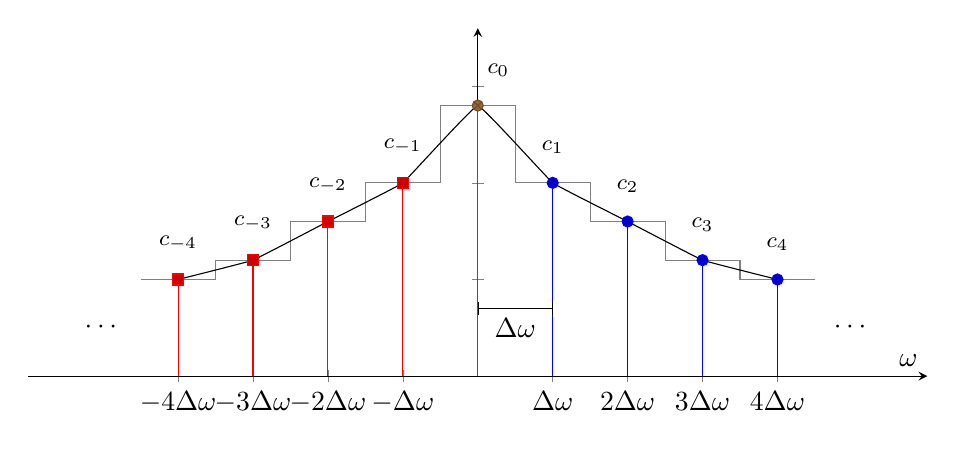
\begin{tikzpicture}
      \begin{axis}[width=13cm,height=6cm,ymin=-0,xmin=-3,ymax=1.8,xmax=3,  yticklabels={,,},
          xtick={-2,-1.5,-1,-0.5,0,0.5,1.0,1.5,2},
          xticklabels={$-4\Delta \omega$,$-3\Delta \omega$,$-2\Delta \omega$,$-\Delta \omega$,$0$,$\Delta \omega$,$2\Delta \omega$,$3\Delta \omega$,$4\Delta \omega$},
          xlabel=$\omega$, axis lines = center]

        \addplot+[ycomb] plot coordinates {(0.5,1) (1.0,0.8) (1.5,0.6) (2,0.5)};
        \addplot+[ycomb] plot coordinates {(-0.5,1) (-1.0,0.8) (-1.5,0.6) (-2,0.5)};
        \addplot+[ycomb] plot coordinates {(0.0, 1.4)};
        \node at (axis cs:-2.5,0.25) {$\cdots$};
        \node at (axis cs:2.5,0.25) {$\cdots$};
        \node at (axis cs:0.25,0.25) {$\Delta \omega$};


        %    \addplot [dimen] plot coordinates {(0.0,0.35) (0.5,0.35)};
        %    \addplot  plot coordinates {(0.0,0.35) (0.5,0.35)};
        \addplot[dimen]  plot coordinates {(0.0,0.35) (0.5,0.35)};
        \addplot[mark=none,color=gray] plot coordinates {(-2.25,0.5) (-1.75,0.5) (-1.75,0.6) (-1.25,0.6) (-1.25,0.8) (-.75,0.8) (-.75,1) (-.25,1) (-.25,1.4) (.25,1.4) (.25,1) (.75,1) (.75,0.8) (1.25,0.8) (1.25,0.6) (1.75,0.6) (1.75,0.5) (2.25,0.5)} ;

        \addplot[mark=none,color=black] plot [smooth,tension=0.1] coordinates {(-2.,0.5) (-1.5,0.6) (-1,0.8) (-.5,1) (0,1.4) (.5,1.) (1,0.8) (1.5,0.6) (2,0.5) } ;

        \node at (axis cs:0.0,1.5) [above right, font={\footnotesize}]{$c_0$};
        \node at (axis cs:0.5,1.1) [above, font={\footnotesize}]{$c_1$};
        \node at (axis cs:1.0,0.9) [above, font={\footnotesize}]{$c_2$};
        \node at (axis cs:1.5,0.7) [above, font={\footnotesize}]{$c_3$};
        \node at (axis cs:2.0,0.6) [above, font={\footnotesize}]{$c_4$};

        \node at (axis cs:-0.5,1.1) [above, font={\footnotesize}]{$c_{-1}$};
        \node at (axis cs:-1.0,0.9) [above, font={\footnotesize}]{$c_{-2}$};
        \node at (axis cs:-1.5,0.7) [above, font={\footnotesize}]{$c_{-3}$};
        \node at (axis cs:-2.0,0.6) [above, font={\footnotesize}]{$c_{-4}$};
      \end{axis}
    \end{tikzpicture}
  \end{center}
  \caption{A depiction of how the Fourier series can be seen as a Riemann sum approximation of an integral of a continuous function.}
\end{figure}

We now inspect the case where $T\rightarrow \infty$. When the period of the
function $x_{T}(t)$ approaches infinity,
we drop the subscript $T$ in the notation and denote it with $x(t)$.
The Riemann sum then approaches the following integral
equation ($\Delta\omega \rightarrow d\omega$, $k\Delta\omega \rightarrow \omega$):
\begin{align}
  \lim_{T\rightarrow \infty} x_{T}(t) & = \lim_{T\rightarrow \infty}\frac{1}{2\pi} \sum_{k=-\infty}^{\infty} \hat{x}_{T}(k\Delta \omega) e^{ik\Delta \omega t}\Delta\omega \\
                                      & =\frac{1}{2\pi}\int_{-\infty}^{\infty} \left[\int_{-\infty}^{\infty} x(t) e^{-i\omega t} dt\right] e^{i\omega t}d\omega            \\
                                      & = \frac{1}{2\pi} \int_{-\infty}^{\infty} \hat{x}(\omega) e^{i\omega t}d\omega                                                      \\
                                      & = x(t) \,\,.
\end{align}
This integral is known as the inverse Fourier transform. It allows us to go from a continuous function $\hat{x}(\omega)$,
which is the continuous spectral representation of the signal, to the time domain signal $x(t)$.

The innermost integral that allows us to obtain $\hat{x}(\omega)$ from the continuous-time signal $x(t)$ is:
\begin{align}
  \hat{x}(\omega) & = \int_{-\infty}^{\infty} x(t) e^{-i\omega t} dt \,\,.
\end{align}
This is the forward Fourier transform.

\newthought{The forward Fourier transform} is defined as:

\begin{equation}
  \boxed{
    \hat{x}(\omega) = \int_{-\infty}^{\infty} x(t) e^{-i\omega t}dt
  } \,\,.
\end{equation}

\newthought{The inverse Fourier transform} is defined as:

\begin{equation}
  \boxed{
    x(t) = \frac{1}{2\pi}\int_{-\infty}^{\infty} \hat{x}(\omega) e^{i\omega t}d\omega
  } \,\,.
\end{equation}
Just as the Fourier series, the continuous-time Fourier transform is in most practical cases invertible.

We'll use the following notation to indicate Fourier transform pairs:
\begin{equation}
  \boxed{
    x(t) \xleftrightarrow{\mathcal{F}} \hat{x}(\omega)
  } \,\,.
\end{equation}
We'll return to the Fourier transform later and show that the Fourier series is a special case of the Fourier transform!

\section{The spectrum of an audio signal}

The Python program in Listing \ref{lst:audio_spec} shows how to use the Fast Fourier Transform (FFT)
command in Python to analyze an audio signal for its spectral contents.
The output of this program is shown in Figure \ref{fig:audio_spec}.

The FFT algorithm is used to evaluate a discrete-time Fourier transform.
This operation is mathematically defined as follows:
\begin{equation}
  c[k] = \sum_{t=0}^{N-1} x[t] e^{-i\frac{2\pi}{N}kt} \,\,.
\end{equation}
Here $c[k]$ is the complex amplitude corresponding to a spectral component with angular frequency $\omega_k = 2\pi k/(T_s N)$, where $T_s=1/f_s$ is the sample-spacing, which is the inverse of the sample-rate of the signal.

You can think of an FFT as a discrete-time equivalent of the Fourier series analysis equation, 
which finds the Fourier series coefficients for a periodic discrete-time signal. 
We will cover the discrete Fourier transform and discrete-time signals in more detail later on, 
I just wanted to already expose you to the FFT algorithm at this point.

\lstinputlisting[language=Python, caption={\texttt{013\_audio\_spec/audio\_spec.py}}, label=lst:audio_spec]{code/013_audio_spec/audio_spec.py}

\begin{figure}
  \begin{center}
    %\includegraphics[width=0.67\textwidth]{ch03/guitar_str.png}
    \includegraphics[width=\textwidth]{code/013_audio_spec/audio_spec.png}
  \end{center}
  \caption{The spectral components of an audio signal (guitar string plucked). Left: time domain signal $x(t)$, Right: The magnitude of the spectral components in decibel scale: $10\log_{10}(|c_k|^2)$.}
  \label{fig:audio_spec}
\end{figure}

\input{ch07/exercises7}
 \ifSpExerciseSol
 % Author: Jørn Olav Jensen

\newpage
\section{Suggested solutions: Fourier Series}

\begin{enumerate}
  % Exercise 1
  \item Let $x(t)$ be the signal:
        \[ x(t) = 7\sin(3\pi t+0.2\pi) + 3\cos(7\pi t+0.5\pi). \]

        \begin{enumerate}[a)]
          % Exercise 1a)
          \item Have that:
                \begin{align*}
                  \sin\theta & =\frac{1}{2i}(e^{i\theta}-e^{-i\theta}), \\
                  \cos\theta & =\frac{1}{2}(e^{i\theta}+e^{-i\theta}).
                \end{align*}
                This gives:
                \begin{align*}
                  x(t) & = \frac{7}{2i}(e^{i(3\pi t+0.2\pi)}-e^{-i(3\pi t+0.2\pi)})+ \frac{3}{2}(e^{i(7\pi t+0.5\pi)}+e^{-i(7\pi t+0.5\pi)}),                                                                                   \\
                       & = \left(\frac{7}{2i}e^{i0.2\pi}\right)e^{i3\pi t}-\left(\frac{7}{2i}e^{-i0.2\pi}\right)e^{-i3\pi t} + \left(\frac{3}{2}e^{i0.5\pi}\right)e^{i7\pi t}+\left(\frac{3}{2}e^{-i0.5\pi}\right)e^{-i7\pi t},
                \end{align*}
                giving:
                \[ c_{k} = \left(\frac{3}{2}e^{-i0.5\pi},-\frac{7}{2i}e^{-i0.2\pi},\frac{7}{2i}e^{i0.2\pi},\frac{3}{2}e^{i0.5\pi}\right), \]
                for which the corresponding angular frequencies are:
                \[ \omega_{k}=(-7\pi,-3\pi,3\pi,7\pi). \]

          % Exercise 1b)
          \item For any real signal, the Fourier coefficients satisfy $c_{-k}=c_{k}^{*}$ and $x(t)$ is real.

          % Exercise 1c)
          \item The signal is periodic if $\omega_{i}/\omega_{j}\in\mathbb{Q}$ for every 
                pair $i,j\in \{-7,-3,3,7\}$ with $i\neq j$. In this case every $\omega_{i}$ is an 
                integer multiple of $\pi$, so every ratio is a rational number as all the $\pi$ cancel.

          % Exercise 1d)
          \item Using Euclid's algorithm we have:
                \begin{align*}
                   & (3\pi,7\pi),      \\
                   & (3\pi,7\pi-3\pi), \\
                   & (3\pi,4\pi),      \\
                   & (3\pi,4\pi-3\pi), \\
                   & (3\pi,\pi),       \\
                   & (3\pi-\pi,\pi),   \\
                   & (2\pi,\pi),       \\
                   & (2\pi-\pi,\pi),   \\
                   & (\pi,\pi).
                \end{align*}
                Hence, the fundamental angular frequency is $\omega=\pi\ \text{rad/s}$. 
                In units of hertz, we have that $\omega=2\pi f$, so
                \[ f = \frac{\omega}{2\pi}=\frac{\pi}{2\pi}=\frac{1}{2}. \]
                Thus, the fundamental frequency is $f=1/2\ \text{Hz}$.

          % Exercise 1e)
          \item If the fundamental angular frequency is $\omega=\pi$, then the fundamental period is related by $T=2\pi/\omega$, hence
                \[ T = \frac{2\pi}{\omega}=\frac{2\pi}{\pi}=2\ \text{seconds}. \]

          % Exercise 1f)
          \item Define a new signal $y(t)=x(t-\frac{1}{2})$. That is, we delay the signal $x(t)$ by $\frac{1}{2}$. We get:
                \[ y(t) = 7\sin(3\pi \left(t-\frac{1}{2}\right)+0.2\pi) + 3\cos(7\pi \left(t-\frac{1}{2}\right)+0.5\pi). \]
                Simplifying gives:
                \[ y(t) = 7\sin(3\pi t-1.3\pi) + 3\cos(7\pi t-3\pi). \]
                Hence, $\phi_{0} = -1.3\pi$ and $\phi_{1}=-3\pi$.

          % Exercise 1g)
          \item Define another signal $z(t) = x(t) + e^{i\sqrt{2}t+13}$. 
                This new signal is not periodic as the frequencies are not commensurable, since we have a factor of $\sqrt{2}$, 
                the signal is also not real-valued since we don't have a corresponding complex conjugate pair.
        \end{enumerate}

  % Exercise 2
  \item Let $x(t)$ be a signal defined as:
        \[ x(t) = e^{-i(6\pi t+0.3)} + 4e^{i(60\pi t+0.42)} + 4e^{-i(60\pi t+0.42)} + e^{i(6\pi t+0.3)}, \]
        where $t$ is measured in seconds.
        \begin{enumerate}[a)]
          % Exercise 2a)
          \item This signal is real-valued since we have two pairs, each with the same frequency, but different signs. Thus, the signal can be written as a real signal for which it takes the following form:
                \[ x(t) = 8\cos(60\pi t + 0.42) + 2\cos(6\pi t + 0.3). \]
          % Exercise 2b)
          \item In this case, we have the angular frequencies of $\omega_{1}=60\pi$ and $\omega_{2}=6\pi$ for which $\omega_{1}/\omega_{2}=60\pi/6\pi=10$. We get a rational number, so the signal is periodic.
          % Exercise 2c)
          \item To find the fundamental angular frequency, we use Euclid's algorithm. This gives:
                \begin{align*}
                   & (60\pi,6\pi), \\
                   & (54\pi,6\pi), \\
                   & (48\pi,6\pi), \\
                   & (42\pi,6\pi), \\
                   & (36\pi,6\pi), \\
                   & (30\pi,6\pi), \\
                   & (24\pi,6\pi), \\
                   & (18\pi,6\pi), \\
                   & (12\pi,6\pi), \\
                   & (6\pi,6\pi),
                \end{align*}
                therefore, the fundamental angular frequency is $6\pi$ in units of radians per second.

          % Exercise 2d)
          \item The fundamental period is:
                \[ T = \frac{2\pi}{\omega} = \frac{2\pi}{6\pi}=\frac{1}{3}, \]
                hence $T=\frac{1}{3}$ in units of seconds.
        \end{enumerate}

  % Exercise 3
  \item Let the Fourier series coefficients of a periodic signal $x(t)$ with fundamental period $T=1$ be:
        \[c_{k} = \begin{cases}
            \frac{1}{10}, \hspace{2.3cm}\quad k=0, \\
            \frac{1}{\pi k}e^{-i\frac{\pi}{10}k}\sin(\frac{\pi}{10}k),\quad \text{otherwise}.
          \end{cases}\]

        \begin{enumerate}[a)]
          % Exercise 3a)
          \item Using Python, we can implement a simple program for the partial sum with $N=101$. Listing \ref{code:7.3a} shows a way.
                \lstinputlisting[language=Python, caption=Suggested solution to a), label=code:7.3a]{ch07/code/ex7_3a.py}

          % Exercise 3b)
          \item The Fourier coefficients of a delayed signal are related to the undelayed signal by $c_{k}'=e^{-i\frac{2\pi k\tau}{T}}c_{k}$.
                The script in Listing \ref{code:7.3a} can be modified to account for delay. The delayed version is shown in Listing \ref{code:7.3b}.
                \lstinputlisting[language=Python, caption=Suggested solution to b), label=code:7.3b]{ch07/code/ex7_3b.py}

          % Exercise 3c)
          \item Define $y(t)=\frac{d}{dt}x(t)$. If $c_{k}$ are the Fourier coefficients for $x(t)$, then the Fourier coefficients for $y(t)$ is:
                \[ d_{k}(t)=i \frac{2\pi k}{T}c_{k}. \]
                Using Python we have Listing \ref{code:7.3c}.
                \lstinputlisting[language=Python, caption=Suggested solution to c), label=code:7.3c]{ch07/code/ex7_3c.py}

        \end{enumerate}

\end{enumerate}
 \fi
\newpage
\section{Audio Compression Example [Optional]}
In this application example, I'll show you how to estimate the
spectral components of an audio signal and how this can be used for
audio compression. I won't go very deep into either of these
topics. The main idea is to expose you to these concepts.

\newthought{Example: audio compression algorithms often use a sparse spectral
representation of an audio signal}.  The sounds produced by musical
instruments when playing a single note are often good examples of
periodic signals that occur in our daily life. Of course, real signals
are typically not exactly periodic, but for short intervals this
approximation is good.

A good example of this is the signal shown in
Figure \ref{fig:audio_spec}, which depicts the sound signal (instantaneous
relative air pressure at the microphone) emitted by a guitar when one
string is plucked.

A Fourier series approximation of an audio signal is often used in
audio compression, as it is often possible to approximate an audio
signal relatively accurately with relatively few non-zero Fourier
series coefficients. This is the basic idea behind the MP3 audio
compression algorithm\sidenote[][0em]{Yes, there is more to it. Note, that
real world compression algorithms use a lot more tricks, such as
psychoacoustics -- not storing spectral components that humans cannot
hear very well in music. These are outside the scope of this basic
course on signal processing though. However, it is already possible to
achieve significant compression just using the simple idea of
representing the signal only using the $N$ largest amplitude spectral
components. I would wager that most of the compression is achieved
with the sparse spectral representation.}.

The Python code in Listing \ref{lst:audio_compression} demonstrates
audio compression in practice. Understanding the program may require
you to be somewhat familiar with analyzing what computer programs
do. If you are just starting with programming, feel free to skip going
through this program example.

The audio compression example program relies on the discrete Fourier
transform (FFT), which we haven't covered yet. Just think of
the \verb|numpy.fft.fft| operation as the analysis step of the Fourier
series, which gives you the phase and amplitude of each frequency
component $c_k$. We'll cover the discrete Fourier transform in more
detail at a later part of this course.

\lstinputlisting[language=Python,caption={\texttt{010\_audio\_compression/audio\_compression.py}},label=lst:audio_compression]{code/010_audio_compression/audio_compression_simple.py}

The algorithm discards weak spectral components of the signal and
stores the strong ones. This can result in significant savings in
storage space. In this example, the amount of storage required is only
5\% of the original audio signal!


\input{Applications/image_comp}
%Equation \ref{eq:dirac_comb_coeff} provides the formula for the phase and amplitude of each spectral component of a Dirac comb signal. What does this result tell you about how power is distributed over frequency?

%\item Using Section \ref{dirac_section}, implement a program that calculates a partial sum approximation of a Dirac delta train with period $T=0.5$ seconds. Use $N=50$ as the number of complex exponential signals to include in the partial sum. Evaluate the signal from t=0 to t=4 seconds at 10 kHz sample rate. Here's some partial code, which almost does the job. 
%\begin{lstlisting}[language=Python,numbers=none]
%# determine sample rate (Hz) sample_rate=10000.0 # create time array 0
%to 4 seconds t=n.arange(4.0*sample_rate)/sample_rate # initialize
%empty vector to hold Fourier series
%sig=n.zeros(len(t),dtype=n.complex) N=50 for k in range(-N,N): sig+=
%...
%    
%plt.plot(sig.real)
%plt.show()
%\end{lstlisting}
%\item[b)] Delay the signal by 0.1 seconds by applying a phasor term to the Fourier series coefficients, with the help of Section \ref{delay_section}. Plot the undelayed and delayed signals in the same plot and verify that the signal is delayed by the right amount.
%\end{itemize}

%\if
\newpage
\section{Variable star lightcurve fitting [Optional]}
\newthought{Example: The study of astronomical light curves of variable stars is an example of a practical application of the Fourier series}.

Variable stars, called Cepheids, have intensities $I(t)$ that vary
periodically as a function of time. An example of a light curve is
shown in Figure \ref{fig:cepheid_lightcurve}. Such variable stars
pulsate in luminosity in a regularly repeating manner. The repeating
luminosity waveform is often very non-sinusoidal, necessitating a
Fourier series analysis.

\begin{marginfigure}
\begin{center}
\includegraphics[width=\textwidth]{Applications/figures/ceph.jpg}
\end{center}
\caption{Measurements of the intensity of a variable star (red) and a Fourier series model of the intensity of the star as a function of time (blue). Illustration Credit: NASA, ESA and Z. Levay (STScI). Science Credit: NASA, ESA, the Hubble Heritage Team (STScI/AURA) and the American Association of Variable Star Observers.}
\label{fig:cepheid_lightcurve}
\end{marginfigure}

Measurements of the intensity of a \emph{\index{Cepheid variable
star}{Cepheid variable star}} are made at periods of time when
telescope time is available and astronomical seeing allows
observations to be made. The time spacing between measurements is
therefore by no means regular.

When analyzing the periodic waveform of this star, a search is made to
determine the period $T$ of the intensity waveform, and the Fourier
series coefficients $c_k$. This is done by using an exhaustive search
for plausible values of $T$. The model function is a Fourier series
synthesis equation:
\begin{equation}
I_N(t) = \sum_{k=-N}^N c_k e^{i\frac{2\pi}{T}kt} \,\,.
\end{equation}
The relationship between luminosity and the pulsation period is
thought to follow a relatively well known relationship that can be
linked to fundamental pulsation frequencies of rotating
stars\cite{hindsley1989period}. Longer period Cepheids are brighter,
as show in Figure \ref{fig:ceph_bright}. This makes these types of
variable stars useful for measuring the astronomical distances.

\begin{marginfigure}
  \begin{center}
    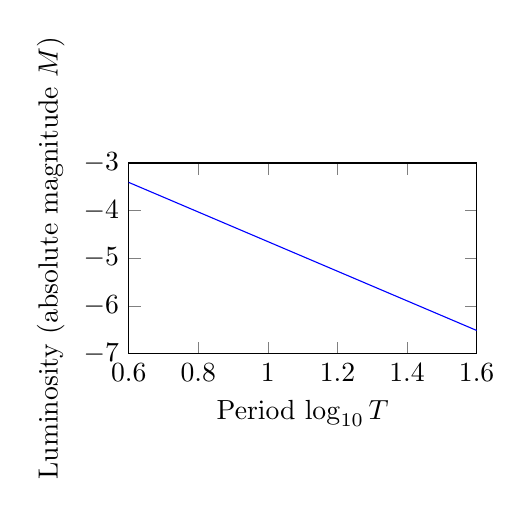
\begin{tikzpicture} \begin{axis}[width=6cm,height=4cm,ymin=-7,ymax=-3,xmin=0.6,xmax=1.6,
          xlabel={Period $\log_{10} T$},
          ylabel={Luminosity (absolute magnitude $M$)}]

        \addplot[samples=400,mark=none,color=blue]{-3.11*(x-0.8)-4.03};

      \end{axis}
    \end{tikzpicture}
  \end{center}
  \caption{Relationship between Cepheid period and absolute magnitude, based on relationship published by Hindsley and Bell (1989).}
  \label{fig:ceph_bright}
\end{marginfigure}

\if 0
\begin{figure}
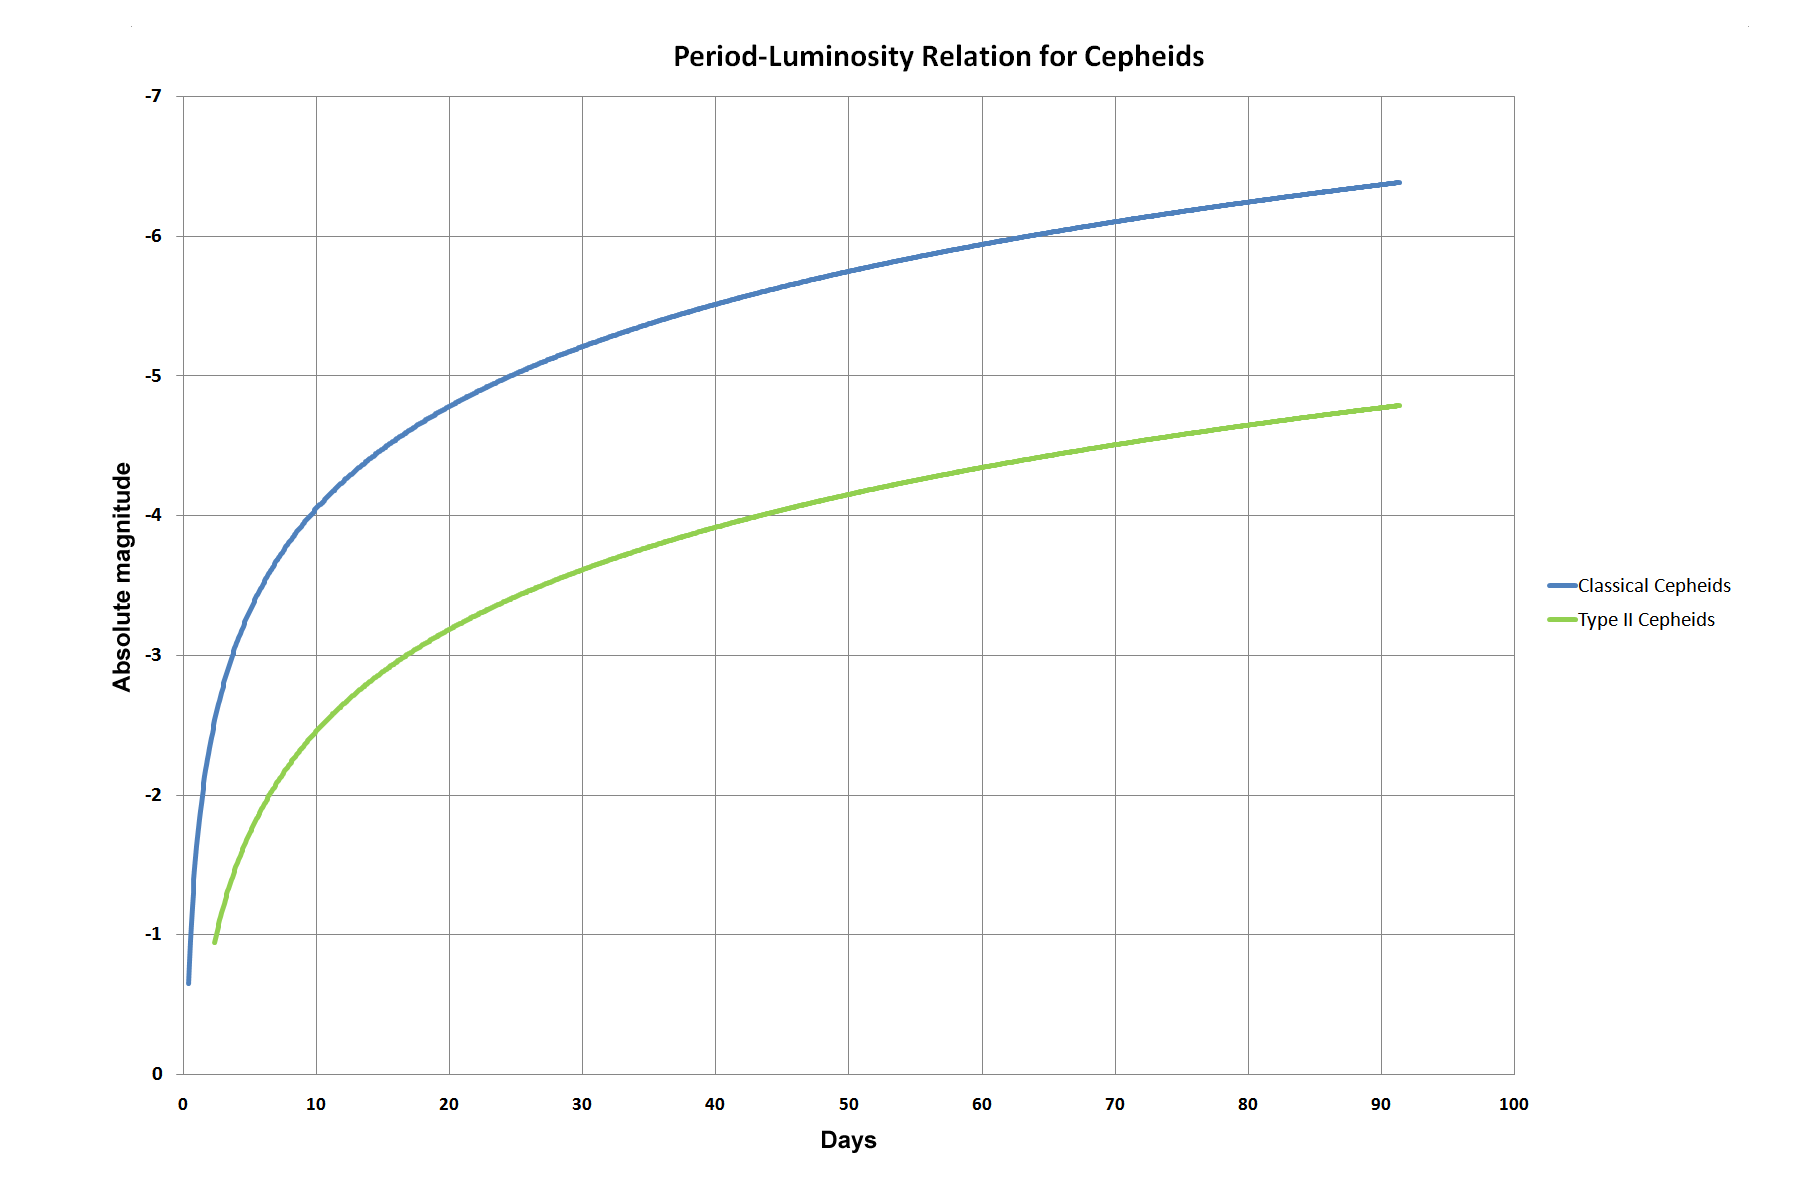
\includegraphics[width=\textwidth]{Applications/figures/ceph_brightness.png}
\caption{Relationship between Cepheid period and absolute magnitude. Figure credit: Vedran V, Wikipedia.}
\label{fig:ceph_bright}
\end{figure}
\fi

The Fourier series can be used to express periodic functions. One real
life use case is estimating the functional form for a periodic star,
which varies in brightness periodically. In this exercise, we will
determine the Fourier series coefficients for brightness observations
of a real Cepheid star. We will then plot the Fourier series for the
periodic light curve of this star.

To estimate the periodic waveform for a Cepheid variable star
brightness measurements $m(t)$, we will use something called the
maximum likelihood method, which estimates the Fourier series
coefficients.  This involves expressing the Fourier series as a matrix
vector operation:
\begin{align}
m &= A x\\
\begin{bmatrix}
m(t_0)\\
m(t_1)\\
m(t_2)\\
\vdots \\
m(t_{M})
\end{bmatrix} &=
\begin{bmatrix}
e^{i\frac{2\pi}{T} k_0 t_0} & e^{i\frac{2\pi}{T} k_1 t_0} & \hdots & e^{i\frac{2\pi}{T} k_N t_0} \\
e^{i\frac{2\pi}{T} k_0 t_1} & e^{i\frac{2\pi}{T} k_1 t_1} & \hdots & e^{i\frac{2\pi}{T} k_N t_1} \\
\vdots & \vdots & \ddots & \vdots \\
e^{i\frac{2\pi}{T} k_0 t_M} & e^{i\frac{2\pi}{T} k_1 t_M} & \hdots & e^{i\frac{2\pi}{T} k_N t_M} 
\end{bmatrix} 
\begin{bmatrix}
c_0 \\
c_1 \\
c_2 \\
\vdots \\
c_N
\end{bmatrix}  \,\,.
\end{align}
Here $c_k$ is a Fourier series coefficient and $T$ is the fundamental
period. Because there are discrete measurements, the measurement
function is only known at discrete points $m(t_{\ell})$. In order to
estimate the Fourier series coefficients, we use the linear
least-squares estimator:
\begin{equation}
\hat{x} = (A^H A)^{-1}A^H m \,\,.
\end{equation}
The vector $\hat{x}$ will now contain the most probable Fourier series
coefficients that explain the measurements $m(t_{\ell})$ of the
periodic function.

Because this course does not deal with statistics, we have implemented
the code that figures out the Fourier series coefficients that fit the
measurements. Your task is to edit the code below, and to evaluate the
Fourier series model, given the coefficients $c_k$, which are in the
array variable named \verb|c_k|. Code is shown in Listing
\ref{lst:variable_star}, which already does most of the work. Complete
the last for-loop, and you should get the following plot:
\begin{center}
\includegraphics[width=0.92\textwidth]{Applications/figures/ceph.png}
\end{center}

\lstinputlisting[language=Python,caption={\texttt{012\_variable\_star/variable\_star.py}},label=lst:variable_star]{code/012_variable_star/variable_star.py}



\fi

\ifSpProgA
\input{Assignments/prog1}
\fi

\ifSpFourierTra
\chapter{Fourier Transform}
\input{ch08/text8}
\input{ch08/exercises8}
 \ifSpExerciseSol
 \input{ch08/solutions8}
 \fi
\input{Applications/am_radio}
\input{Applications/rc_circuit}
\fi

\ifSpDT
\chapter{Discrete-time Signals}
\begin{marginfigure}
  \begin{center}
    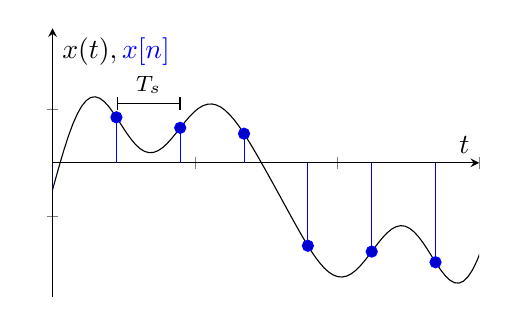
\begin{tikzpicture}
      \begin{axis}[domain=-2*3.1415:2*3.1415,
        width=7cm,height=5cm,ymin=-2.5,xmin=0,ymax=2.5,xmax=6,
        ytick={-1,1},
        yticklabels={,,},
        xticklabels={,,},
        ylabel={$x(t),{\color{blue}x[n]}$},
        xlabel=$t$, axis lines = center]
        \addplot+[ycomb,samples=15] {-0.5+sin(deg(x))+0.5*sin(2*deg(0.5*x)-0.0)+0.7*sin(3*deg(x)-0.6)+0.3*sin(4*deg(x)+1.6)};
        \addplot[samples=200]{-0.5+sin(deg(x))+0.5*sin(2*deg(0.5*x)-0.0)+0.7*sin(3*deg(x)-0.6)+0.3*sin(4*deg(x)+1.6)};
        \node at (axis cs:0.9+0.45,1.1) [above, font={\footnotesize}]{$T_s$};
        \addplot [dimen,black]plot coordinates {(0.9,1.1) (2.0*0.9,1.1)};
      \end{axis}\
    \end{tikzpicture}
  \end{center}
  \caption{A continuous-time signal $x(t)$, and a discrete-time signal
    $x[n]$. Sample-spacing $T_s$ is related to sample-rate as follows:
    $T_s = 1/f_s$.}

\end{marginfigure}
In this chapter, we introduce discrete-time signals. These are the
type of signals that are used for digital signal processing. We'll
cover the following topics:
\begin{itemize}
  \item Discretization
  \item Aliasing
  \item Oversampling and undersampling
  \item Reconstruction
  \item Shannon-Nyquist sampling theorem
\end{itemize}
We'll need to know about complex sinusoidal signals and the frequency
domain representation of signals (the Fourier transform).

\section{Sampling}
\begin{marginfigure}
  \tikzstyle{int}=[draw, minimum size=2em]
  \tikzstyle{init} = [pin edge={to-,thin,black}]
  \begin{center}
    %  \resizebox{\columnwidth}{!}{%
    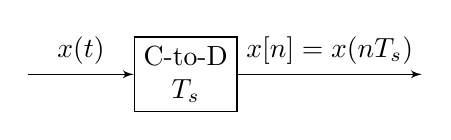
\begin{tikzpicture}[every text node part/.style={align=center},node distance=3cm,auto,>=latex']
      \node [int] (a) {C-to-D \\ $T_s$};
      \node (b) [left of=a,node distance=2cm, coordinate] {a};
      %    \node (c) [below=a,node distance=3cm] {a};

      %\node [int, pin={[init]above:$p_0$}] (c) [right of=a] {$\frac{1}{s}$};
      \node [coordinate] (end) [right of=a, node distance=3cm]{};
      \path[->] (b) edge node {$x(t)$} (a);
      %\path[->] (a) edge node {$v$} (c);
      \draw[->] (a) edge node {$x[n]=x(nT_s)$} (end) ;
    \end{tikzpicture}
    % }
  \end{center}
  \caption{An ideal continuous-time to Discrete-time (C-to-D) converter.}
\end{marginfigure}


A continuous-time signal can be converted into a discrete-time signal
by sampling it. This can be idealized as a system that performs the following operation:
\begin{equation}
  \boxed{
    x[n] = x(n T_s)
  }\,\,.
\end{equation}
In this process, a continuous function $x(t) \in \mathbb{C}$ is converted into an ordered 
sequence of numbers $x[n] \in \mathbb{C}$, where $n\in\mathbb{Z}$ indicates the order of the numbers.

The reason why we consider complex-valued signals in addition to real-valued signals is 
that there are many applications where the signals are naturally complex-valued. 
Radio signal processing is one example.

The \index{sample-spacing}{sample-spacing} $T_s$ determines how densely samples of the 
continuous-time signal are taken. Sample-spacing is related with the \index{sample-rate}{sample-rate} 
or \index{sampling-rate}{sampling-rate} $f_s$ as follows:
\begin{equation}
  \boxed{
    f_s = \frac{1}{T_s}
  }\,\,.
\end{equation}
Sample-rate typically is given in units of samples per second or hertz, but other units are also used in various applications.
For example, the resolution of a digital image is often given in units of dots per inch (DPI).

\if 0 You can think of sampling as a convolution operation between a
  time-shifted unit impulse $\delta(t-nT_s)$ and the continuous-time
  signal $x(t)$:
  \begin{align}
    x[n] & = \int_{-\infty}^{\infty} x(\tau) \delta(n T_s - \tau)  d\tau \\
         & = x(n T_s)\,\,.
  \end{align}
\fi

\subsection{Sampling a complex sinusoidal signal}
In order to understand sampling, you need to understand how sampling affects a complex sinusoidal signal:
\begin{equation}
  x(t)=A e^{i\phi} e^{i\omega_0 t}\,\,.
\end{equation}
Because we can use the Fourier transform to represent signals as a superposition of complex 
sinusoidal signals, knowledge of what happens to a fixed frequency signal will tell us how 
discretization affect signals more generally.

\begin{marginfigure}
  \begin{center}
    \begin{tikzpicture}
      \begin{axis}[width=7cm,height=6cm,ymin=0,xmin=-3,ymax=1.5,xmax=3,  yticklabels={,,},
          xtick={1.0},
          ylabel={$\hat{x}(\omega)$},
          xticklabels={$\omega_0$},
          xlabel=$\omega$, axis lines = center]

        \addplot + [ycomb] plot coordinates {(1,1)};
        \node at (axis cs:1,1.1) [above, font={\footnotesize}]{$Ae^{i\phi}$};
      \end{axis}
    \end{tikzpicture}
  \end{center}
\end{marginfigure}

So what happens to a complex sinusoidal signal when we sample it?
\begin{align}
  x[n] & =x(nT_s)                                \\
       & =A e^{i\phi} e^{i\omega_0 n T_s }       \\
       & =A e^{i\phi} e^{i\hat{\omega}_0 n}\,\,.
\end{align}
What happens is that we get a discrete-time complex sinusoidal signal. This signal has a special type of frequency:
\begin{equation}
  \boxed{
    \hat{\omega}_0 = \omega_0 T_s
  }\,\,.
\end{equation}

The angular frequency $\hat{\omega}_0$ is called a \emph{\index{discrete-time angular frequency}{discrete-time angular frequency}}.
It indicates how many \emph{\index{radians per sample}{radians per sample}} the phase of 
the complex sinusoidal signal advances. With a discrete-time signal, time is only 
implied from the sample spacing that was used to discretize the signal, which is 
why no time unit is attached to $\hat{\omega}_0$. There's a hat on $\hat{\omega}_0$ 
to signify that this is not the same kind of frequency as the continuous-time angular 
frequency $\omega$, which has units of radians per second.

Figure \ref{fig:rotating_dt_phasor} shows an example of how the values of the discrete-time complex 
sinusoidal signal behave with increasing sample index, obtaining values on a circle of 
radius $A$ in the complex plane. The amount of angle per sample that the signal advances for
each sample on the circle is given by the discrete-time angular frequency $\hat{\omega}_0$.

\begin{marginfigure}
  \begin{center}
    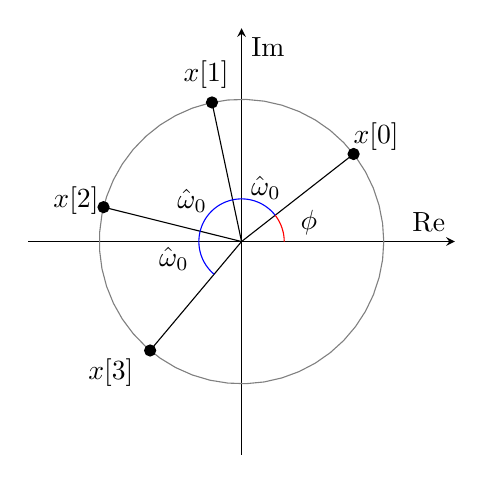
\begin{tikzpicture}
      \pgfmathsetmacro{\PHI}{38}
      \pgfmathsetmacro{\OM}{64}
      \begin{axis}[axis equal, disabledatascaling,
          ymin=-1.5,xmin=-1.5,ymax=1.5,xmax=1.5, ticks=none,
          xlabel=$\mathrm{Re}$, ylabel=$\mathrm{Im}$, axis lines = center,
          width=7cm, height=7cm]
        % unit circle
        \addplot [gray,domain=0:2*pi,samples=50]({cos(deg(x))},{sin(deg(x))});
        % first sample
        \addplot [black, mark = *] coordinates {( {cos(\PHI)}, {sin(\PHI)} )} {};
        \addplot [black] coordinates { (0,0) ( {cos(\PHI)}, {sin(\PHI)} ) };

        % second sample
        \addplot [black, mark = *] coordinates {( {cos(\OM+\PHI)}, {sin(\OM+\PHI)} )} {};
        \addplot [black] coordinates { (0,0) ( {cos(\OM+\PHI)}, {sin(\OM+\PHI)} ) };

        % third sample
        \addplot [black, mark = *] coordinates {( {cos(2*\OM+\PHI)}, {sin(2*\OM+\PHI)} )} {};
        \addplot [black] coordinates { (0,0) ( {cos(2*\OM+\PHI)}, {sin(2*\OM+\PHI)} ) };

        % third sample
        \addplot [black, mark = *] coordinates {( {cos(3*\OM+\PHI)}, {sin(3*\OM+\PHI)} )} {};
        \addplot [black] coordinates { (0,0) ( {cos(3*\OM+\PHI)}, {sin(3*\OM+\PHI)} ) };

        \node at (axis cs:{1.2*cos(\PHI)},{1.2*sin(\PHI)}) {$x[0]$};
        \node at (axis cs:{1.2*cos(\OM+\PHI)},{1.2*sin(1*\OM+\PHI)}) {$x[1]$};
        \node at (axis cs:{1.2*cos(2*\OM+\PHI)},{1.2*sin(2*\OM+\PHI)}) {$x[2]$};
        \node at (axis cs:{1.2*cos(3*\OM+\PHI8)},{1.2*sin(3*\OM+\PHI)}) {$x[3]$};


        \addplot [red,domain=0:(pi*\PHI/180),samples=50]({0.3*cos(deg(x))},{0.3*sin(deg(x))});
        \node at (axis cs:{0.5*cos(\PHI/2.0)},{0.4*sin(\PHI/2.0)}) {$\phi$};

        \addplot [blue,domain=(pi*\PHI/180):(pi*(\PHI+\OM)/180),samples=50]({0.3*cos(deg(x))},{0.3*sin(deg(x))});
        \node at (axis cs:{0.5*cos((\PHI+\PHI+\OM)/2)},{0.4*sin((\PHI+\PHI+\OM)/2)}) {$\hat{\omega}_0$};

        \addplot [blue,domain=(pi*(\PHI+\OM)/180):(pi*(\PHI+2*\OM)/180),samples=50]({0.3*cos(deg(x))},{0.3*sin(deg(x))});
        \node at (axis cs:{0.5*cos((\PHI+\OM + \PHI+2*\OM)/2)},{0.4*sin((\PHI+\OM + \PHI+2*\OM)/2)}) {$\hat{\omega}_0$};

        \addplot [blue,domain=(pi*(\PHI+2*\OM)/180):(pi*(\PHI+3*\OM)/180),samples=50]({0.3*cos(deg(x))},{0.3*sin(deg(x))});
        \node at (axis cs:{0.5*cos((\PHI+2*\OM + \PHI+3*\OM)/2)},{0.4*sin((\PHI+2*\OM + \PHI+3*\OM)/2)}) {$\hat{\omega}_0$};

      \end{axis}
    \end{tikzpicture}
  \end{center}
  \caption{A discretized complex sinusoidal signal $x[n] = A e^{i\phi}e^{i\hat{\omega}_0n}$ 
  with phase increments of $\hat{\omega}_0$ radians per sample. The initial phase for sample $n=0$ is given by $\phi$.}
  \label{fig:rotating_dt_phasor}
\end{marginfigure}

\subsection{Frequency aliases}
What happens if $\hat{\omega}$ gets larger? What if it is so large that the phasor rotates 
around the circle on the complex plane one or more times every sample? 
This phenomenon is called aliasing.

Here's a more formal way of defining aliasing. The complex sinusoidal
signal $e^{i\hat{\omega}_0 n}$ is not unique. There are infinitely
many possible frequency increments that result in the same signal:
\begin{align}
  x[n] & =Ae^{i\phi} e^{i(\hat{\omega}_0 + 2\pi k) n} \\
       & =Ae^{i\phi} e^{i \hat{\omega}_0  n}
\end{align}
where $k\in\mathbb{Z}$. What this means is that we can select any one
of the discrete-time angular frequencies:
\begin{equation}
  \boxed{
    \hat{\omega}_k = \hat{\omega}_0 + 2\pi k
  }\,\,.
\end{equation}
and our discrete-time complex sinusoidal signal will be
identical. There is no way of telling just from the signal itself what
the true discrete-time angular frequency is. Frequencies
$\hat{\omega}_k$ are called \emph{\index{aliases}{aliases}}. There are
infinitely many such aliases.

\begin{marginfigure}[5cm]
  \begin{center}
    \begin{tikzpicture}
      \begin{axis}[
          width=7cm,
          height=6cm,
          ymin=0,
          xmin=-4,
          ymax=1.2,
          xmax=4,
          yticklabels={,,},
          xtick={-3.6,-1.6, .4, 2.4},
          xticklabels={$f_0-2 f_s $,$f_0- f_s$,$f_0$,$f_0+f_s$},
          xlabel=$f$,
          ylabel=$\hat{x}(f)$,
          axis lines = center]
        \addplot+[ycomb] plot coordinates {((-3.6,1) (-1.6,1) (0.4,1) (2.4,1)};
      \end{axis}
    \end{tikzpicture}
  \end{center}
  \caption{Each one of these signals $Ae^{i\phi}e^{i2\pi (f_0 + k f_s)t}$
  would result in the same discrete-time complex sinusoidal signal
  when discretized with sample-rate $f_s$. Note that we're showing the
  spectrum with continuous-time frequency in units of hertz (cycles
  per second) instead of radians per second.}
\end{marginfigure}

What continuous-time frequencies do these aliases correspond to? We
can work this out by looking at the continuous-time signal of
frequency $\omega_0$:
\begin{equation}
  x(t) = A e^{i\phi} e^{i\omega_0 t}\,\,.
\end{equation}
When discretized, each of the following signals are identical:
\begin{align}
  x[n] & =A e^{i\phi} e^{i \omega_0 T_s n }                \\
       & = A e^{i\phi} e^{i(\omega_0 T_s + 2\pi k) n }     \\
       & = A e^{i\phi} e^{i(\omega_0 + 2\pi k/T_s) T_s n } \\
       & = A e^{i\phi} e^{i(\omega_0 + 2\pi k f_s) T_s n } \\
       & = A e^{i\phi} e^{i \omega_k T_s n } \,\,.
\end{align}
We've used the relationship between sample-rate $f_s=1/T_s$ and sample
spacing here. The aliases map to continuous-time angular frequency as
follows:
\begin{equation}
  \boxed{
    \omega_k = \omega_0 + 2\pi k f_s
  }\,\,
\end{equation}

Any one of these continuous-time angular frequencies $\omega_k$ would
result in an identical discrete-time complex sinusoidal signal when
discretized with sample-rate $f_s$. Dividing by
$2\pi$, we get the aliasing behavior in units of hertz (samples per
second)\footnote{remember that angular frequency (radians per second)
  and frequency (cycles per second) are related as follows $\omega = 2\pi
    f$.}:
\begin{equation}
  \boxed{
    f_k = f_0 + k f_s
  }\,\,.
\end{equation}
The phenomena of aliasing is problematic. We cannot uniquely distinguish
a discrete-time complex sinusoidal signal $x[n]=Ae^{i\hat{\omega}n}$
which continuous-time signal it corresponds to. Conversely,
there are infinitely many continuous-time sinusoidal signals
$x(t)=Ae^{i\omega t}$ that will result in the same discrete-time
signal. In order to rule out the wrong solutions, we need a priori
information about the spectral occupancy of the continuous-time
signal.

\begin{marginfigure}
  \begin{center}
    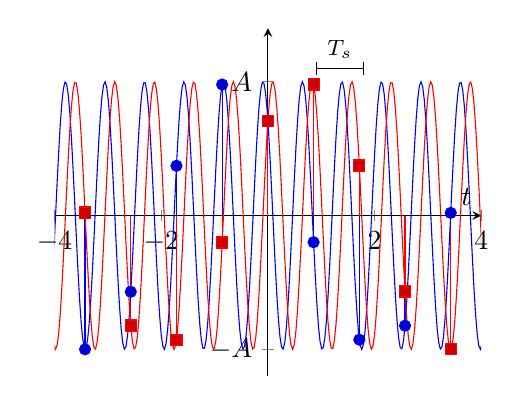
\begin{tikzpicture}
      \begin{axis}[domain=-6:6,
          width=7cm,height=6cm,ymin=-1.2,xmin=-4,ymax=1.4,xmax=4,
          ytick={-1,1},
          yticklabels={$-A$, $A$},
          xlabel=$t$, axis lines = center]
        \addplot+[ycomb,samples=15,color=blue]{cos(deg(2.0*3.1415*1.35*x+3.14/4))};
        \addplot+[ycomb,samples=15,color=red]{sin(deg(2.0*3.1415*1.35*x+3.14/4))};

        \addplot[samples=400,blue]{cos(deg(2.0*3.1415*1.35*x+3.14/4))};
        \addplot[samples=400,red]{sin(deg(2.0*3.1415*1.35*x+3.14/4))};
        %            \addplot[samples=400,color=red]{cos(deg(2.0*3.1415*0.18333333333333335*x+3.14/4))};
        %           \addplot[samples=400,color=green]{cos(deg(2.0*3.1415*0.9833333333333334*x-3.14/4))};


        \node  at (axis cs:0.9+0.45,1.1) [above, font={\footnotesize}]{$T_s$};
        \addplot [dimen,black]plot coordinates {(0.9,1.1) (2.0*0.9,1.1)};
      \end{axis}

    \end{tikzpicture}
    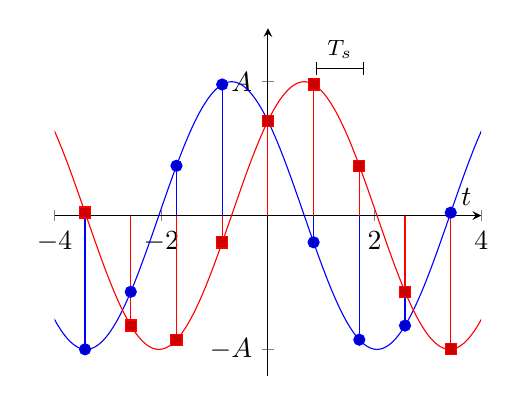
\begin{tikzpicture}
      \begin{axis}[domain=-6:6,
          width=7cm,height=6cm,ymin=-1.2,xmin=-4,ymax=1.4,xmax=4,
          ytick={-1,1},
          yticklabels={$-A$, $A$},
          xlabel=$t$, axis lines = center]
        %            \addplot[samples=400,blue]{cos(deg(2.0*3.1415*1.35*x+3.14/4))};
        \addplot+[ycomb,samples=15,color=blue]{cos(deg(2.0*3.1415*0.18333333333333335*x+3.14/4))};
        \addplot+[ycomb,samples=15,color=red]{sin(deg(2.0*3.1415*0.18333333333333335*x+3.14/4))};
        \addplot[samples=400,color=blue]{cos(deg(2.0*3.1415*0.18333333333333335*x+3.14/4))};
        \addplot[samples=400,color=red]{sin(deg(2.0*3.1415*0.18333333333333335*x+3.14/4))};
        %            \addplot[samples=400,color=green]{cos(deg(2.0*3.1415*0.9833333333333334*x-3.14/4))};


        \node  at (axis cs:0.9+0.45,1.1) [above, font={\footnotesize}]{$T_s$};
        \addplot [dimen,black]plot coordinates {(0.9,1.1) (2.0*0.9,1.1)};
        %\addplot[color=black] plot coordinates {(0.9,1.1) (2.0*0.9,1.1)};
      \end{axis}
    \end{tikzpicture}
  \end{center}
  \caption{Two different complex sinusoidal signals that result in the same discrete-time signal.}
\end{marginfigure}

Solving the problem of aliasing, by ensuring that there is a uniquely one-to-one mapping 
between continuous-time and discrete-time frequencies for all the spectral components 
of a signal, leads to the Shannon-Nyquist sampling theorem, which is introduced at the end of this chapter.

\subsection{Real-valued signals}
The concept of aliasing of complex sinusoidal signals allows us to inspect aliasing of 
real-valued sinusoidal signals, which come in pairs of positive and negative frequency 
spectral components. Understanding aliasing for real-valued signals is slightly more 
complicated than understanding complex-valued signals, because of the symmetric 
pairing of the positive and negative frequency components.

The Fourier transform of a real-valued signal $x(t)\in\mathbb{R}$ is conjugate symmetric
\begin{equation}
  \hat{x}(\omega) = \hat{x}^*(-\omega)\,\,.
\end{equation}
This means that real-valued signals are composed of conjugate
symmetric pairs of positive and negative frequency spectral
components:
\begin{equation}
  A \cos(\omega t + \phi) = \frac{A}{2}(e^{i\phi}e^{i\omega t} + e^{-i\phi}e^{-i\omega t})\,\,.
\end{equation}
In order to understand how aliasing affects real-valued signals, we
need to investigate how pairs of positive and negative frequency spectral components are affected.
\begin{marginfigure}
  \begin{center}
    \begin{tikzpicture}
      \begin{axis}[width=7cm,height=6cm,ymin=0,xmin=-2,ymax=1.5,xmax=2,  yticklabels={,,},
          xtick={-1, 1.0},
          xticklabels={$-\omega_0$,$\omega_0$},
          ylabel=$\hat{x}(\omega)$,
          xlabel=$\omega$,
          axis lines = center]

        \addplot+[ycomb] plot coordinates {(1,1)};
        \addplot+[ycomb] plot coordinates {(-1,1)};

        \node at (axis cs:1,1.1) [above, font={\footnotesize}]{$\frac{A}{2}e^{i\phi}$};
        \node at (axis cs:-1,1.1) [above, font={\footnotesize}]{$\frac{A}{2}e^{-i\phi}$};
      \end{axis}
    \end{tikzpicture}
  \end{center}
  \caption{A real-valued signal consists of a positive and negative frequency spectral component, 
  which are conjugate symmetric.}
\end{marginfigure}
A conjugate symmetric pairing of positive and negative frequencies means that there is no 
distinction between a positive and a negative frequency signal\footnote{For complex 
sinusoidal signals $e^{-i \omega t}$ and $e^{i \omega t}$ are two unique signals.}.
For example, let's say we have a signal with angular frequency $\omega = -0.1$:
\begin{equation}
  A \cos(-0.1 t + \phi) = \frac{A}{2}(e^{i\phi}e^{-i0.1  t} + e^{-i\phi}e^{i0.1 t})\,\,.
\end{equation}
This is the same thing as a cosine signal with frequency $0.1$, but a sign flipped phase:
\begin{align}
  \frac{A}{2}(e^{-i\phi}e^{i 0.1 t} + e^{i\phi}e^{-i 0.1 t}) & = A \cos(0.1 t - \phi)       \\
                                                             & = A \cos(-0.1 t + \phi)\,\,.
\end{align}
This means that you can always represent a real-valued sinusoidal signal using only 
positive valued frequencies, but it does not apply for complex-valued signals.

In the case of real-valued signals, the frequency alias corresponding to a negative 
frequency is called a \emph{\index{folded alias}{folded alias}}. For complex sinusoidal 
signals, a folded alias does not exist, as positive and negative frequency 
components are not necessarily paired.

\subsection{Example: Sinusoidal signal with $f_0=1$ Hz and $f_s=10$ Hz}
\begin{marginfigure}
  \begin{center}
    \includegraphics[width=\textwidth]{code/014_sampling/aliased_signals.png}
  \end{center}
  \caption{Example of signal aliasing for $f_0\in \{-19,-9,1,11,21\}$
    Hz and $f_s=10$ Hz. All signals alias identically. Python code:
    \texttt{014\_sampling/aliasing\_example.py}.}
\end{marginfigure}

Consider the following sinusoidal signal with a frequency of $f_0 =1$ Hz and phase $\phi$:
\begin{align}
  x(t) & =A\cos(2\pi f_0 t + \phi)  \\
  x(t) & =A\cos(2\pi t + \phi)\,\,.
\end{align}
When discretized with a sample-rate $f_s=10$ Hz or $T_s=1/f_s = 0.1$ s this becomes:
\begin{align}
  x[n] & =x(nT_s)                     \\
       & =A\cos(2\pi n T_s + \phi),   \\
       & =A\cos(0.2\pi n + \phi)\,\,.
\end{align}
The discrete-time angular frequency is $\hat{\omega}_0 = 0.2\pi$. 
For any $k\in\mathbb{Z}$ this signal is identical to:
\begin{align}
  x[n] & =A\cos([0.2\pi + 2\pi k] n + \phi)\,\,.
\end{align}
In discrete-time angular frequencies (radians per sample), the aliases are:
\begin{align}
  \hat{\omega}_k & = (0.2\pi+2\pi k)                                   \\
                 & =\ldots,-3.8\pi,-1.8\pi,0.2\pi,2.2\pi,4.2\pi,\ldots
\end{align}
In continuous-time frequency (Hz), the aliases would be:
\begin{align}
  f_k & =f_0 + f_s k                     \\
      & =\ldots,-19,-9,1,11,21,31,\ldots
\end{align}
In other words, a discretized cosine signal produced from any of the frequencies $f_k$ 
would be identical to a 1 Hz signal, when using 10 Hz sample rate. The negative solutions 
are called folded aliases, which can be interpreted as cosine signals with positive 
frequencies $9,19,\cdots$ but with a sign flipped phase.

\begin{figure}
  \begin{center}
    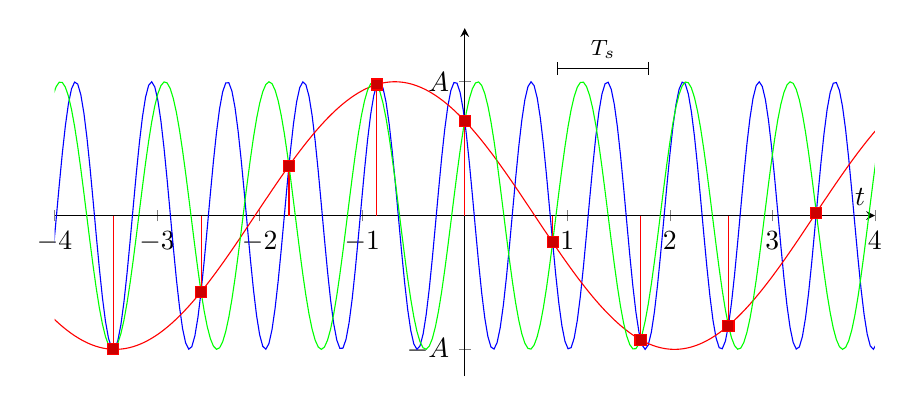
\begin{tikzpicture}
      \begin{axis}[
          domain=-6:6,
          width=12cm,
          height=6cm,
          ymin=-1.2,
          xmin=-4,
          ymax=1.4,
          xmax=4,
          ytick={-1,1},
          yticklabels={$-A$, $A$},
          xlabel=$t$,
          axis lines = center]
        \addplot[samples=400,blue]{cos(deg(2.0*3.1415*1.35*x+3.14/4))};
        \addplot+[ycomb,samples=15,color=red]{cos(deg(2.0*3.1415*1.35*x+3.14/4))};
        \addplot[samples=400,color=red]{cos(deg(2.0*3.1415*0.18333333333333335*x+3.14/4))};
        \addplot[samples=400,color=green]{cos(deg(2.0*3.1415*0.9833333333333334*x-3.14/4))};

        \node at (axis cs:0.9+0.45,1.1) [above, font={\footnotesize}]{$T_s$};
        \addplot[dimen,color=black] plot coordinates {(0.9,1.1) (2.0*0.9,1.1)};
      \end{axis}
    \end{tikzpicture}
  \end{center}
  \caption{The following figure illustrates what the continuous-time and discrete-time signals 
  look like. They are all identical in discrete-time, because the continuous-time signals 
  intersect at the sampling points. The red line shows $\omega_0 = 0.2\pi f_s$ (1 Hz), 
  the green line shows $\omega_1 = -1.8\pi f_s$ (-9 Hz), and the blue line shows $\omega_2=2.2\pi f_s$ (11 Hz).
  One can also see the phase-flip on the negative frequency folded alias, shown in green.
  The blue and red continuous-time signals are both sampled at identical phases, but the green not.}
\end{figure}

Figure \ref{fig:dt_spec_ex} shows part of the discrete-frequency
spectrum where there are three aliases of the cosine signal. There are infinitely many aliases, but only three are shown here.
It is customary to call the region of the spectrum where $|\hat{\omega}| < \pi$ or $|f| < f_s/2$, the \emph{principal spectrum}.
This region of the spectrums contains the smallest discrete-time angular frequency aliases.
\begin{figure}
  \begin{center}
    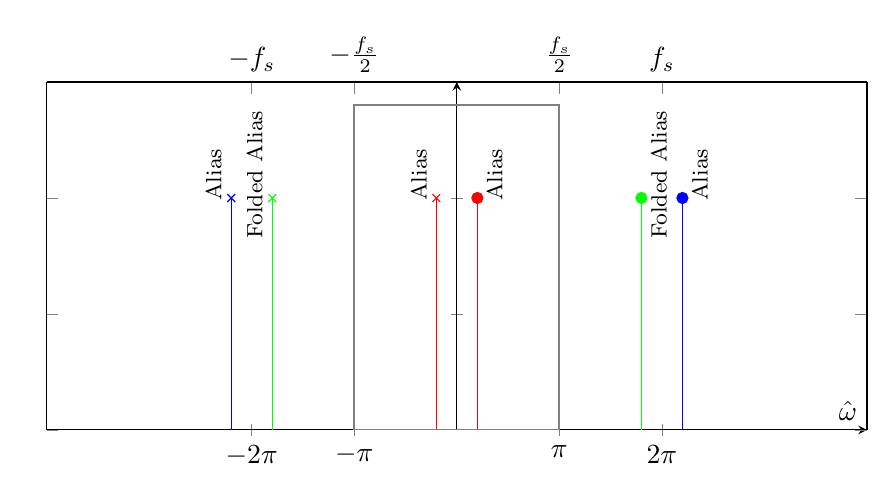
\begin{tikzpicture}
      \begin{axis}[width=12cm,height=6cm,ymin=0,xmin=-4,ymax=1.5,xmax=4,  yticklabels={,,},
          xtick={-2,-1,1,2},
          xticklabels={$-2\pi$,$-\pi$,$\pi$,$2\pi$},
          xlabel=$\hat{\omega}$, axis lines = center]

        \addplot[ycomb,color=blue,mark=*,mark color=blue] plot coordinates {(2.2,1)};
        \addplot[ycomb,color=green,mark=*,mark color=green] plot coordinates { (1.8,1)};
        \addplot[ycomb,color=red,mark=*,mark color=red] plot coordinates { (0.2,1)};

        \addplot[ycomb,color=blue,mark=x,mark color=blue] plot coordinates {(-2.2,1)};

        \addplot[ycomb,color=green,mark=x,mark color=green] plot coordinates {(-1.8,1)};

        \addplot[ycomb,color=red,mark=x,mark color=red] plot coordinates {(-0.2,1)};

        \node at (axis cs:0.2,1.1) [below, rotate=90, font={\footnotesize}]{Alias};
        \node at (axis cs:-0.2,1.1) [above, rotate=90, font={\footnotesize}]{Alias};
        \node at (axis cs:1.8,1.1) [below, rotate=90, font={\footnotesize}]{Folded Alias};
        \node at (axis cs:-1.8,1.1) [above, rotate=90, font={\footnotesize}]{Folded Alias};

        \node at (axis cs:2.2,1.1) [below, rotate=90, font={\footnotesize}]{Alias};
        \node at (axis cs:-2.2,1.1) [above, rotate=90, font={\footnotesize}]{Alias};

        \draw [gray, thick] (axis cs:-1,0.0) rectangle (axis cs:1,1.4);
      \end{axis}
      \begin{axis}[
          width=12cm,
          height=6cm,
          ymin=0,
          xmin=-4,
          ymax=1.5,
          xmax=4,
          yticklabels={,,},
          xlabel={},
          xtick={-2,-1,1,2},
          xticklabels={$-f_s$,$-\frac{f_s}{2}$,$\frac{f_s}{2}$,$f_s$},
          axis x line*=top]

      \end{axis}
    \end{tikzpicture}
  \end{center}
  \caption{Spectral aliases of the components plotted as a function of
    discrete-time angular frequency $\hat{\omega}$ (radians per
    sample). The pairing of positive and negative frequencies indicates
    that this signal is real-valued, and that the $\hat{\omega}_{-1} =
      -1.8\pi$ alias corresponds to a cosine signal with a positive
    discrete-time angular frequency of $1.8\pi$ and a flipped
    phase. Frequency in units of hertz is shown on the top axis.}
  \label{fig:dt_spec_ex}
\end{figure}

How could we be able to determine which one of the frequencies $f_k$ is the true sinusoidal 
frequency component represented by the discrete-time signal? We can only do this if we know 
that the continuous-time frequencies of the spectral components of the signal lie within a certain range.

For example, if we knew that there are no spectral components with frequencies higher than 5 
Hz present in the continuous-time signal ($|f| < 5$) Hz, then we could determine that the discrete-time 
signal is due to a 1 Hz continuous-time signal, because this is the only possible mapping between a 
discrete-time frequency and a continuous-time frequency.

\subsection{Principal spectrum}
The \emph{\index{principal spectrum}{principal spectrum}} (also called normalized angular frequency) 
is the range of discrete-time angular frequencies between:
\begin{equation}
  \boxed{-\pi < \hat{\omega} < \pi}\,\,.
\end{equation}
It is the region for the lowest frequency discrete-time angular frequency representation for 
discrete-time spectral components that the signal consists of. 
Unaliased continuous-time frequencies between
\begin{equation}
  -f_s/2 < f < f_s/2
\end{equation}
in units of hertz are mapped to this range of discrete-time angular frequencies.

By finding a suitable value for $k$, it is possible to find an alias of any discrete-time angular frequency $\hat{\omega}$,
which lands in the range $-\pi< \hat{\omega}+2\pi k < \pi$. This is called the \emph{\index{principal alias}{principal alias}}.
Every spectral component of a signal has an alias in the principal spectrum.

\newthought{For example}, consider a signal of frequency $f=123$ Hz:
\begin{equation}
  x(t) =\cos( 2\pi f t) = \frac{1}{2}(e^{i 2\pi f t}+e^{-i 2\pi f t})\,\,,
\end{equation}
which is sampled using a sample-rate of $f_s=100$. The discrete-time angular frequency is 
$\hat{\omega} = \pm 2\pi \cdot 123 \cdot\frac{1}{100} = \pm 2.46\pi$. 
This is outside the principal spectrum. If we shift this by $\mp 2\pi$, we obtain principal aliases:
$\hat{\omega} = \pm 0.46 \pi$.

\subsection{Folding}
Figure \ref{fig:ti_folding} shows an illustration by Texas Instruments, 
which nicely describes the concept of folding of spectral components.

\begin{marginfigure}[-4cm]
  \begin{center}
    \includegraphics[width=\textwidth]{ch09/figures/folding.JPG}
  \end{center}
  \caption{Folding.}
  \label{fig:ti_folding}
\end{marginfigure}

Folding implies that at frequencies between $[f_s/2+k f_s,f_s + kf_s]$ with $k=0,1,2,\ldots$, 
the order of the spectral components are flipped. Note that this only occurs if the signal is real-valued,
as folding relies on a pairing of positive and negative frequency spectral components.

\newthought{The following example demonstrates folding using three real-valued sinusoidal signals}. 
Let us consider three sinusoidal signals:
\begin{align}
  x_1(t) & = A\cos(2\pi f_0 t), \\
  x_2(t) & = A\cos(2\pi f_1 t), \\
  x_3(t) & = A\cos(2\pi f_2 t),
\end{align}
with frequencies:
\begin{align}
  f_0 & = 0.1 f_s,     \\
  f_1 & = 0.2 f_s,     \\
  f_2 & = 0.3 f_s\,\,.
\end{align}
When we discretize these signals, we obtain:
\begin{align}
  x_0[n] & = A\cos(2\pi f_0 n/f_s) = A\cos(0.2\pi n), \\
  x_1[n] & = A\cos(2\pi f_1 n/f_s) = A\cos(0.4\pi n), \\
  x_2[n] & = A\cos(2\pi f_2 n/f_s) = A\cos(0.6\pi n).
\end{align}
These signals have spectral components with discrete-time angular frequencies 
within the principal spectrum:
\begin{align}
  \hat{\omega}_0 & =\pm 0.2\pi, \\
  \hat{\omega}_1 & =\pm 0.4\pi, \\
  \hat{\omega}_2 & =\pm 0.6\pi.
\end{align}
If we now take three more sinusoidal signals, with frequencies:
\begin{align}
  f_3 & = 0.7 f_s, \\
  f_4 & = 0.8 f_s, \\
  f_5 & = 0.9 f_s.
\end{align}
When discretized we obtain the following principal aliases:
\begin{align}
  x_3[n] & = A\cos(2\pi f_3 n/f_s) = A\cos(1.4\pi n) = A\cos(-0.6\pi n),     \\
  x_4[n] & = A\cos(2\pi f_4 n/f_s) = A\cos(1.6\pi n) = A\cos(-0.4\pi n),     \\
  x_5[n] & = A\cos(2\pi f_5 n/f_s) = A\cos(1.8\pi n) = A\cos(-0.2\pi n)\,\,.
\end{align}
The frequencies $f_3$, $f_4$, and $f_5$ have the following aliases within the principal spectrum:
\begin{align}
  \hat{\omega}_3 & =\mp 0.6\pi      \\
  \hat{\omega}_4 & =\mp 0.4\pi      \\
  \hat{\omega}_5 & =\mp 0.2\pi\,\,.
\end{align}
If we inspect the ordering of the frequencies, we can see that $|f_0|<|f_1|<|f_2|$. 
This agrees with $|\hat{\omega}_0|<|\hat{\omega}_1|<|\hat{\omega}_2|$.
However, when we compare the ordering $|f_3|<|f_4|<|f_5|$, we can see that the order 
is reversed with respect to $|\hat{\omega}_5|<|\hat{\omega}_4|<|\hat{\omega}_3|$. This is due to folding.

\begin{marginfigure}
  \begin{center}
    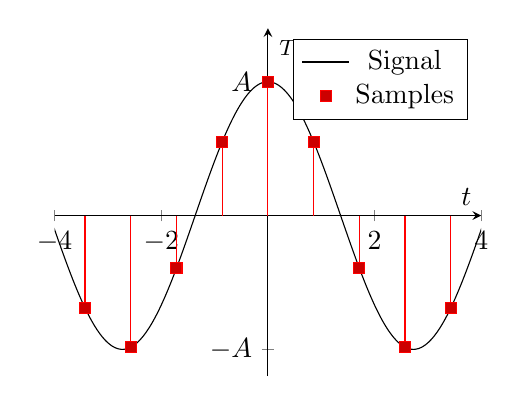
\begin{tikzpicture}
      \begin{axis}[domain=-6:6,
          width=7cm,height=6cm,ymin=-1.2,xmin=-4,ymax=1.4,xmax=4,
          ytick={-1,1},
          legend pos=north east,
          yticklabels={$-A$, $A$},
          xlabel=$t$, axis lines = center]
        \addplot[samples=400]{cos(deg(2.0*3.1415*0.18333333333333335*x))};
        \addplot+[ycomb,samples=15]{cos(deg(2.0*3.1415*0.18333333333333335*x))};
        \node at (axis cs:0.45,1.1) [above, font={\footnotesize}]{$T_s$};
        \addplot[dimen] plot coordinates {(0.9,1.1) (2.0*0.9,1.1)};
        \legend{Signal,Samples}
      \end{axis}
    \end{tikzpicture}

    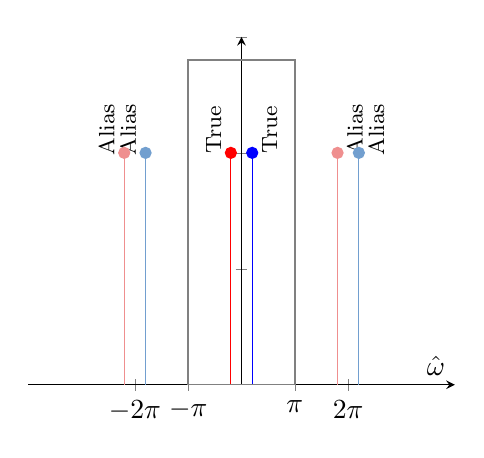
\begin{tikzpicture}
      \begin{axis}[width=7cm,height=6cm,ymin=0,xmin=-4,ymax=1.5,xmax=4,  yticklabels={,,},
          xtick={-2,-1,1,2},
          xticklabels={$-2\pi$,$-\pi$,$\pi$,$2\pi$},
          xlabel=$\hat{\omega}$, axis lines = center]

        \addplot[ycomb,color=blue,mark=*,mark color=blue] plot coordinates {(0.2,1)};
        \addplot[ycomb,color=skyblue1,mark=*,mark color=skyblue] plot coordinates { (-1.8,1)};
        \addplot[ycomb,color=skyblue1,mark=*,mark color=skyblue] plot coordinates { (2.2,1)};

        \addplot[ycomb,color=red,mark=*,mark color=red] plot coordinates {(-0.2,1)};

        \addplot[ycomb,color=scarletred1,mark=*,mark color=scarletred1] plot coordinates {(1.8,1)};

        \addplot[ycomb,color=scarletred1,mark=*,mark color=scarletred1] plot coordinates {(-2.2,1)};

        \node at (axis cs:0.2,1.1) [below, rotate=90, font={\footnotesize}]{True};
        \node at (axis cs:-0.2,1.1) [above, rotate=90, font={\footnotesize}]{True};
        \node at (axis cs:1.8,1.1) [below, rotate=90, font={\footnotesize}]{Alias};
        \node at (axis cs:-1.8,1.1) [above, rotate=90, font={\footnotesize}]{Alias};

        \node at (axis cs:2.2,1.1) [below, rotate=90, font={\footnotesize}]{Alias};
        \node at (axis cs:-2.2,1.1) [above, rotate=90, font={\footnotesize}]{Alias};

        \draw [gray, thick] (axis cs:-1,0.0) rectangle (axis cs:1,1.4);
      \end{axis}
    \end{tikzpicture}
  \end{center}
  \caption{Oversampling $f_s > 2 f_0$.}
  \label{fig:oversampling}
\end{marginfigure}

% The figure below illustrates this case
\begin{marginfigure}
  \begin{center}
    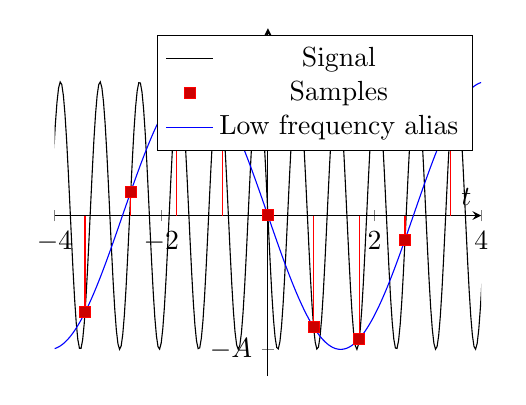
\begin{tikzpicture}
      \begin{axis}[domain=-6:6,
          width=7cm,height=6cm,ymin=-1.2,xmin=-4,ymax=1.4,xmax=4,
          ytick={-1,1},
          yticklabels={$-A$, $A$},
          xlabel=$t$, axis lines = center]
        \addplot[samples=400]{cos(deg(2.0*3.1415*1.35*x+3.14/2))};
        \addplot+[ycomb,samples=15]{cos(deg(2.0*3.1415*1.35*x+3.14/2))};
        \addplot[samples=400,color=blue]{cos(deg(2.0*3.1415*0.18333333333333335*x+3.14/2))};
        \node at (axis cs:0.9+0.45,1.1) [above, font={\footnotesize}]{$T_s$};
        \addplot[color=black] plot coordinates {(0.9,1.1) (2.0*0.9,1.1)};
        \legend{Signal,Samples,Low frequency alias}
      \end{axis}
    \end{tikzpicture}
    %\end{center}
    %The discrete-frequency spectrum of the signal is shown below:
    %\begin{center}
    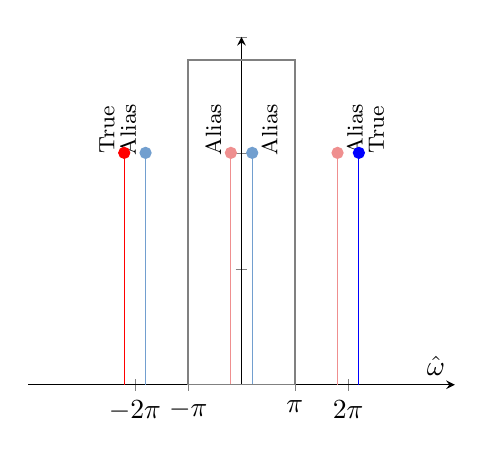
\begin{tikzpicture}
      \begin{axis}[width=7cm,height=6cm,ymin=0,xmin=-4,ymax=1.5,xmax=4,  yticklabels={,,},
          xtick={-2,-1,1,2},
          xticklabels={$-2\pi$,$-\pi$,$\pi$,$2\pi$},
          xlabel=$\hat{\omega}$, axis lines = center]

        \addplot[ycomb,color=blue,mark=*,mark color=blue] plot coordinates {(2.2,1)};
        \addplot[ycomb,color=skyblue1,mark=*,mark color=skyblue] plot coordinates { (-1.8,1)};
        \addplot[ycomb,color=skyblue1,mark=*,mark color=skyblue] plot coordinates { (0.2,1)};

        \addplot[ycomb,color=red,mark=*,mark color=red] plot coordinates {(-2.2,1)};

        \addplot[ycomb,color=scarletred1,mark=*,mark color=scarletred1] plot coordinates {(1.8,1)};

        \addplot[ycomb,color=scarletred1,mark=*,mark color=scarletred1] plot coordinates {(-0.2,1)};

        \node at (axis cs:0.2,1.1) [below, rotate=90, font={\footnotesize}]{Alias};
        \node at (axis cs:-0.2,1.1) [above, rotate=90, font={\footnotesize}]{Alias};
        \node at (axis cs:1.8,1.1) [below, rotate=90, font={\footnotesize}]{Alias};
        \node at (axis cs:-1.8,1.1) [above, rotate=90, font={\footnotesize}]{Alias};

        \node at (axis cs:2.2,1.1) [below, rotate=90, font={\footnotesize}]{True};
        \node at (axis cs:-2.2,1.1) [above, rotate=90, font={\footnotesize}]{True};

        \draw [gray, thick] (axis cs:-1,0.0) rectangle (axis cs:1,1.4);
        %   \node at (axis cs:-0.4,1.1) [above, font={\footnotesize}]{$\frac{A}{2}e^{i\phi}$};
        %  \node at (axis cs:2.4,1.1) [above, font={\footnotesize}]{$\frac{A}{2}e^{-i\phi}$};
        % \node at (axis cs:-2.4,1.1) [above, font={\footnotesize}]{$\frac{A}{2}e^{i\phi}$};
      \end{axis}
    \end{tikzpicture}
  \end{center}
  \caption{Undersampling $f_s < f_0$. When the sample rate is smaller than the frequency of the 
  sinusoid there is less than one sample per sinusoid cycle. The discrete-time frequency 
  $\hat{\omega}>2\pi$ and a low-frequency alias of the high frequency sinusoid exists 
  in the principal spectrum.}
  \label{fig:undersampling}
\end{marginfigure}

\subsection{Nyquist oversampling criterion}
Let us assume that our continuous-time signal has non-zero spectral components with 
frequencies only within the range $|f|<\frac{1}{2}f_s$. This means that it has a 
Fourier transform representation of the form:
\begin{equation}
  x(t) = \frac{1}{2\pi}\int_{-\pi f_s}^{\pi f_s} \hat{x}(\omega)
  e^{i\omega t}d\omega\,\,.
\end{equation}
When such a signal is discretized, all the discrete-time spectral components of the 
signal land on the principal spectrum between $-\pi <\hat{\omega} < \pi$.

The band limited nature of the continuous-time signal also guarantees that no high frequency 
components will have low frequency aliases in the principal spectrum.
In this case, one can be certain that there is a one-to-one mapping between discrete-time 
frequency and continuous-time frequency. And therefore, no information is lost when discretizing the signal. 
In this case, the signal is said to be \emph{\index{oversampled}{oversampled}}.

To avoid aliasing of spectral component frequencies $f>f_s/2$ into the principal spectrum, 
the sample rate $f_s$ has to be at least twice the frequency of the highest frequency 
component of the signal:
\begin{equation}
  \boxed{
    f_s > 2f_{\mathrm{max}}
  }\,\,.
\end{equation}
It can be also expressed as
\begin{equation}
  \boxed{
    f_{\mathrm{max}}<\frac{1}{2}f_s
  }\,\,.
\end{equation}
This is called the \emph{\index{Nyquist oversampling}{Nyquist oversampling}} criterion. 
It is a special case of the more general Shannon-Nyquist sampling theorem.
If this criterion is not satisfied, then the signal is said to be \emph{undersampled}.

When deriving the Shannon-Nyquist sampling theorem, we will see that it is in some cases 
possible to retain information even when the signal is undersampled. 
Undersampling is a technique that is often used for sampling radio signals.

\newthought{For example}, the Nyquist frequency $f_{\mathrm{max}}$ of a real-valued 
signal sampled at $f_s=44.1$ kHz is $f_{\mathrm{max}}=22.05$ kHz. 
The sample rate 44.1 kHz is often used when digitizing audio, because audio signals 
within the human hearing range are between $0<f<20$ kHz and signals conveying audio 
signals only contain spectral components within this range.

\subsection{Nyquist zones}
\begin{marginfigure}
  \begin{center}
    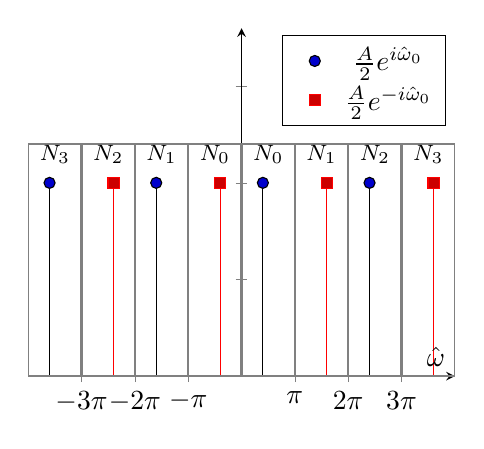
\begin{tikzpicture}
      \begin{axis}[width=7cm,height=6cm,ymin=0,xmin=-4,ymax=1.8,xmax=4,  yticklabels={,,},
          xtick={-3,-2,-1,0,1,2,3},
          xticklabels={$-3\pi$,$-2\pi$,$-\pi$,0,$\pi$,$2\pi$,$3\pi$},
          xlabel=$\hat{\omega}$, axis lines = center]
        \addplot+[ycomb,black] plot coordinates {(0.4,1) (2.4,1) (-1.6,1) (-3.6,1)};
        \addplot+[ycomb,red] plot coordinates {(-0.4,1) (1.6,1) (-2.4,1) (3.6,1)};
        \legend{$\frac{A}{2}e^{i\hat{\omega}_{0}}$,$\frac{A}{2}e^{-i\hat{\omega}_{0}}$};
        \draw [gray, thick] (axis cs:0,0.0) rectangle (axis cs:1,1.2);
        \draw [gray, thick] (axis cs:1,0.0) rectangle (axis cs:2,1.2);
        \draw [gray, thick] (axis cs:2,0.0) rectangle (axis cs:3,1.2);
        \draw [gray, thick] (axis cs:3,0.0) rectangle (axis cs:4,1.2);
        \draw [gray, thick] (axis cs:4,0.0) rectangle (axis cs:5,1.2);
        \draw [gray, thick] (axis cs:-1,0.0) rectangle (axis cs:0,1.2);
        \draw [gray, thick] (axis cs:-2,0.0) rectangle (axis cs:-1,1.2);
        \draw [gray, thick] (axis cs:-3,0.0) rectangle (axis cs:-2,1.2);
        \draw [gray, thick] (axis cs:-4,0.0) rectangle (axis cs:-3,1.2);
        \draw [gray, thick] (axis cs:-5,0.0) rectangle (axis cs:-4,1.2);
        \node at (axis cs:0.5,1.05) [above, font={\footnotesize}]{$N_0$};
        \node at (axis cs:1.5,1.05) [above, font={\footnotesize}]{$N_1$};
        \node at (axis cs:2.5,1.05) [above, font={\footnotesize}]{$N_2$};
        \node at (axis cs:3.5,1.05) [above, font={\footnotesize}]{$N_3$};
        \node at (axis cs:4.5,1.05) [above, font={\footnotesize}]{$N_4$};
        \node at (axis cs:-0.5,1.05) [above, font={\footnotesize}]{$N_0$};
        \node at (axis cs:-1.5,1.05) [above, font={\footnotesize}]{$N_1$};
        \node at (axis cs:-2.5,1.05) [above, font={\footnotesize}]{$N_2$};
        \node at (axis cs:-3.5,1.05) [above, font={\footnotesize}]{$N_3$};
        \node at (axis cs:-4.5,1.05) [above, font={\footnotesize}]{$N_4$};
      \end{axis}
    \end{tikzpicture}
  \end{center}
  \caption{Nyquist zones.}
  \label{fig:nyq_zones}
\end{marginfigure}

If spectral components of a real-valued continuous-time signal are only located 
between $k f_s/2\le|f|<(k+1)f_s/2$ for only one value of $k$ and if there are no 
non-zero spectral components elsewhere, then one can still recover the 
continuous-time signal from the discrete-time representation of the signal,
using the a priori information that the signals are within this range of frequencies. 
This is the more general sampling criterion for real-valued signals.

These regions, which are shown in Figure \ref{fig:nyq_zones}, are called Nyquist zones. 
In each of these cases, all the low frequency aliases of the signal will be confined
with the principal spectrum $\pm \pi$. Because no signals from outside the specific 
Nyquist zone are present, there is no chance of two continuous-time spectral
components mapping to the same normalized angular frequency within the principal spectrum.

\begin{marginfigure}
  \begin{center}
    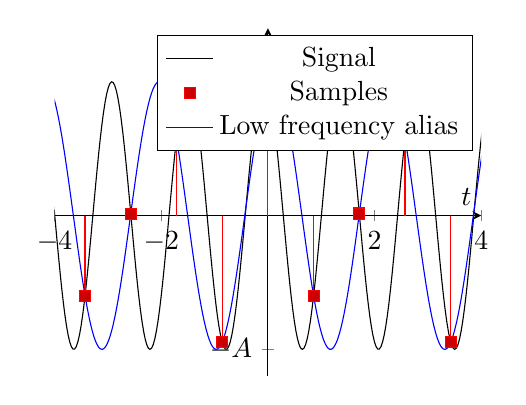
\begin{tikzpicture}
      \begin{axis}[domain=-6:6,
          width=7cm,height=6cm,ymin=-1.2,xmin=-4,ymax=1.4,xmax=4,
          ytick={-1,1},
          yticklabels={$-A$, $A$},
          xlabel=$t$, axis lines = center]
        \addplot[samples=400]{cos(deg(2.0*3.1415*0.7*x+0.3))};
        \addplot+[ycomb,samples=15]{cos(deg(2.0*3.1415*0.7*x+0.3))};
        \addplot[samples=400,color=blue]{cos(deg(2.0*3.1415*0.4666666666666667*x-0.3))};
        \node at (axis cs:0.9+0.45,1.1) [above, font={\footnotesize}]{$T_s$};
        \addplot plot coordinates {(0.9,1.1) (2.0*0.9,1.1)};
        \legend{Signal,Samples,Low frequency alias}
      \end{axis}
    \end{tikzpicture}
  \end{center}

  \begin{center}
    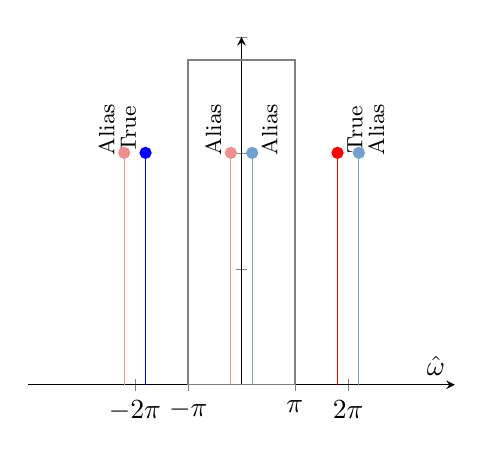
\begin{tikzpicture}
      \begin{axis}[width=7cm,height=6cm,ymin=0,xmin=-4,ymax=1.5,xmax=4,  yticklabels={,,},
          xtick={-2,-1,1,2},
          xticklabels={$-2\pi$,$-\pi$,$\pi$,$2\pi$},
          xlabel=$\hat{\omega}$, axis lines = center]

        \addplot[ycomb,color=blue,mark=*,mark color=blue] plot coordinates {((-1.8,1)};
        \addplot[ycomb,color=skyblue1,mark=*,mark color=skyblue] plot coordinates { (2.2,1)};
        \addplot[ycomb,color=skyblue1,mark=*,mark color=skyblue] plot coordinates { (0.2,1)};

        \addplot[ycomb,color=red,mark=*,mark color=red] plot coordinates {(1.8,1)};

        \addplot[ycomb,color=scarletred1,mark=*,mark color=scarletred1] plot coordinates {(-2.2,1)};

        \addplot[ycomb,color=scarletred1,mark=*,mark color=scarletred1] plot coordinates {(-0.2,1)};

        \node at (axis cs:0.2,1.1) [below, rotate=90, font={\footnotesize}]{Alias};
        \node at (axis cs:-0.2,1.1) [above, rotate=90, font={\footnotesize}]{Alias};
        \node at (axis cs:1.8,1.1) [below, rotate=90, font={\footnotesize}]{True};
        \node at (axis cs:-1.8,1.1) [above, rotate=90, font={\footnotesize}]{True};

        \node at (axis cs:2.2,1.1) [below, rotate=90, font={\footnotesize}]{Alias};
        \node at (axis cs:-2.2,1.1) [above, rotate=90, font={\footnotesize}]{Alias};

        \draw [gray, thick] (axis cs:-1,0.0) rectangle (axis cs:1,1.4);
        %   \node at (axis cs:-0.4,1.1) [above, font={\footnotesize}]{$\frac{A}{2}e^{i\phi}$};
        %  \node at (axis cs:2.4,1.1) [above, font={\footnotesize}]{$\frac{A}{2}e^{-i\phi}$};
        % \node at (axis cs:-2.4,1.1) [above, font={\footnotesize}]{$\frac{A}{2}e^{i\phi}$};
      \end{axis}
    \end{tikzpicture}
  \end{center}
  \caption{Folded undersampling $f_{0} < f_s < 2 f_0$, There are between 1 and 2 samples for each cycle of the continuous-time sinusoid. The low frequency alias is phase flipped.}
  \label{fig:folded_undersampling}
\end{marginfigure}

When $k=0$, this case is called an \emph{oversampled} signal. This is the special case that 
the Nyquist oversampling criterion applies to. When $k = 1$, the signal sampling is 
called \emph{folded undersampled} signal. In this case, the aliased signal 
in the principal spectrum is flipped in frequency and phase relative to the 
continuous-time spectrum. When $k=2$, the signal is \emph{undersampled}. 
These different cases are shown in Figures \ref{fig:oversampling}, 
\ref{fig:folded_undersampling}, and \ref{fig:undersampling}.

There are many cases, especially with modern software defined radios, 
where undersampling or folded undersampling at Nyquist zones $k>0$ are used. 
This violates the simple $f_s > 0.5 f_{\mathrm{max}}$ Nyquist oversampling criterion, 
but is still perfectly fine, as long as the original continuous-time signal has 
spectral components confined within a Nyquist zone.


\subsection{Complex-valued signals}
For complex-valued signals, the \emph{principal spectrum} is the same as it is for 
real-valued signals. In discrete-time angular frequency it is $-\pi<\hat{\omega}<\pi$ and 
in continuous-time frequency $-\frac{1}{2}f_s<f<\frac{1}{2}f_s$. However, because there 
are no conjugate symmetric negative frequency pairs, both negative and positive frequencies 
can be used in this frequency band. Therefore, the effective bandwidth is twice that of 
real-valued signals sampled at the sample rate $f_s$, as both positive and negative 
frequency components can be used independently to encode information.

To ensure a one-to-one relationship between the discrete-time signal and the 
continuous-time signal, the sample rate $f_s$ has to be at least the difference 
between the largest and smallest frequency component
\begin{equation}
  \boxed{
  f_s > f_{\mathrm{max}}-f_{\mathrm{min}}
  }\,\,.
\end{equation}
if the frequency domain representation of the complex-valued signal is within a 
continuous range of frequencies between $f_{\mathrm{min}}$ and $f_{\mathrm{max}}$. 
This avoids having two continuous-time spectral components with different frequencies 
aliasing onto the same discrete-time frequency within the principal 
spectrum\sidenote{The most general sampling criterion involves investigating 
the relationship between the frequency domain representation of the 
continuous-time signal and the frequency domain representation of the 
discretized signal, which we will discuss later when deriving the Shannon sampling theorem.}.
This is another form of the Shannon-Nyquist sampling criterion, 
which applies only to complex-valued signals.

Figure \ref{fig:complex_aliasing} below illustrates aliasing with complex sinusoidal signals. 
Here, a complex sinusoidal signal with frequency $1.2\frac{f_s}{2}$ that is sampled with 
frequency $f_s$ aliases to $-0.8\frac{f_s}{2}$ in the principal spectrum.

\begin{marginfigure}
  \begin{center}
    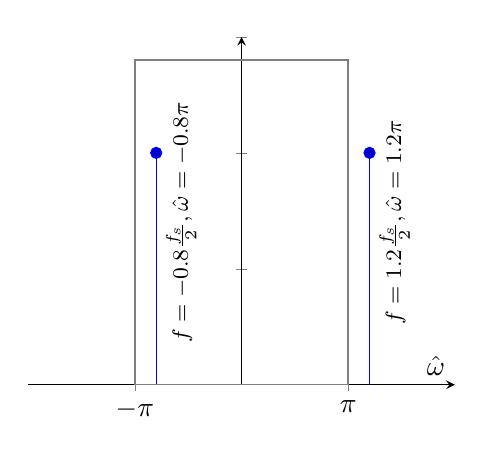
\begin{tikzpicture}
      \begin{axis}[width=7cm,height=6cm,ymin=0,xmin=-2,ymax=1.5,xmax=2,  yticklabels={,,},
          xtick={-1,1},
          xticklabels={$-\pi$,$\pi$},
          xlabel=$\hat{\omega}$, axis lines = center]
        \addplot+[ycomb] plot coordinates {((-0.8,1) (1.2,1)};
        %    \addplot+[ycomb] plot coordinates {(-1.2,1) (0.8,1)};
        \node at (axis cs:1.2,0.7) [below, rotate=90, font={\footnotesize}]{$f=1.2\frac{f_s}{2}, \hat{\omega}=1.2\pi$};
        \node at (axis cs:-0.8,0.7) [below, rotate=90, font={\footnotesize}]{$f=-0.8\frac{f_s}{2}, \hat{\omega}=-0.8\pi$};
        \draw [gray, thick] (axis cs:-1,0.0) rectangle (axis cs:1,1.4);

        %   \node at (axis cs:-0.4,1.1) [above, font={\footnotesize}]{$\frac{A}{2}e^{i\phi}$};
        %  \node at (axis cs:2.4,1.1) [above, font={\footnotesize}]{$\frac{A}{2}e^{-i\phi}$};
        % \node at (axis cs:-2.4,1.1) [above, font={\footnotesize}]{$\frac{A}{2}e^{i\phi}$};
      \end{axis}
    \end{tikzpicture}
  \end{center}
  \caption{Aliasing of a complex sinusoidal spectral component into the principal spectrum. No conjugate symmetric negative frequency spectral components complicate the aliasing of the signal into the principal spectrum.}
  \label{fig:complex_aliasing}
\end{marginfigure}

\newthought{An example of aliasing of two complex sinusoidal signals} is shown below. 
If a continuous-time signal consists of two complex sinusoidal signals:
\begin{equation}
  z(t)=a_1 e^{i 2\pi f_1 t} + a_2 e^{i 2\pi f_2 t}\,\,,
\end{equation}
with frequencies $f_1= 1.2 f_s/2$ and $f_2=0.8 f_s/2$.

When this signal is sampled with a sample-rate of $f_s$, the Nyquist oversampling criterion 
for real-valued signals is violated, because $f_1 > f_s/2$.
However, this is a complex-valued signal, and we only need $f_{\mathrm{max}} - f_{\mathrm{min}} < f_s$ 
to hold in the more general case for complex-valued signals.

This condition is not violated. To see that everything is fine, we
translate both of the sinusoidal signals into the principal spectrum:
\begin{align}
  z[n] & = a_1 e^{i 1.2\pi n }+ a_2 e^{i 0.8\pi n }       \\
       & = a_1 e^{-i 0.8\pi n }+ a_2 e^{i 0.8\pi n }\,\,.
\end{align}
We see that the signals land at $\hat{\omega} = \pm 0.8\pi$ in the
principal spectrum. The two spectral components are distinct, and if we have sufficient information 
about the lowest and highest frequency component of the signal 
(i.e., we know $f_{\mathrm{min}}$ and $f_{\mathrm{max}}$), 
we can still perfectly reconstruct the signal.

\if 0
  For example, if we knew that $f_{\mathrm{min}} = 0$ and $f_{\mathrm{max}} = f_s$, 
  we would know that all spectral components with discrete-time angular frequencies in 
  the principal spectrum between $-\pi$ and $0$ would correspond to continuous-time frequencies 
  between $f_s/2$ and $f_s$. Similarly, we would know that all spectral components with 
  discrete-time angular frequencies between 0 and $\pi$ in the principal spectrum would be 
  mapped to continuous-time frequencies between 0 and $f_s/2$.
\fi

\subsection{2D aliasing}
Consider a two-dimensional signal $I(x,y) \in \mathbb{R}$, which is discretized as follows:

\begin{equation}
  I[n,m]=I(n T_x, m T_y)\,\,.
\end{equation}
Here $T_x$ and $T_y$ are sample spacing in the $x$ and $y$ direction, and $n$, and $m$ are sample 
indices in the two dimensions.

A 2D signal has a spectral representation, which is given by 2D complex exponential signals:
\begin{equation}
  I(x,y) = \frac{1}{(2\pi)^{2}} \int_{-\infty}^{\infty} \int_{-\infty}^{\infty} \hat{I}(\omega_1,\omega_2) e^{i(\omega_1 x + \omega_2 y)} d\omega_1 d\omega_2\,\,.
\end{equation}
\begin{marginfigure}
  \begin{center}
    \includegraphics[width=\textwidth]{ch09/figures/briko.jpg}
    \includegraphics[width=\textwidth]{ch09/figures/brickd.jpg}
  \end{center}
  \caption{Example of aliasing behavior in a 2D image. Above: original, Below: aliased. When scaling an image (reducing its size),
    it is important to apply an anti-aliasing filter that removes high frequency spectral components from the
    high resolution image before it is scaled down to a lower resolution. Otherwise, there is a risk that 
    high frequency periodic structures
    will appear as low frequency structures in the scaled image, as shown in the lower image.
    Anti-aliasing filtering is a standard feature of most image processing libraries, and one rarely 
    sees the type of aliasing shown in the bottom figure in practice.}
  \label{fig:brick_alias}
\end{marginfigure}
To study aliasing behavior in 2D, it is sufficient to study aliasing effects on individual spectral components:
\begin{equation}
  z(x,y) = a e^{i (\omega_1 x + \omega_2 y) }\,\,,
\end{equation}
When discretizing the 2D complex exponential spectral component, one can obtain aliasing behavior 
when sampling through $2\pi$-periodicity:
\begin{align}
  z[n,m] & = a e^{i(\omega_1 T_x n + \omega_2 T_y m ) }                                \\
         & =a e^{i([\omega_1 T_x + 2\pi k]n + [\omega_2 T_y + 2\pi \ell]m)}            \\
         & =a e^{i([\hat{\omega}_1 + 2\pi k]n + [\hat{\omega}_{2} + 2\pi \ell]m)}\,\,.
\end{align}
Here $k,l \in \mathbb{Z}$.

Figure \ref{fig:brick_alias} demonstrates aliasing in 2D. This is
discretized in such a way that the high spatial frequency brick
pattern on the side of the building becomes undersampled, and a low
frequency alias is seen.


\subsection{Reconstruction}
\begin{marginfigure}
  \tikzstyle{int}=[draw, minimum size=2em]
  \tikzstyle{init} = [pin edge={to-,thin,black}]
  \begin{center}
    %  \resizebox{\columnwidth}{!}{%
    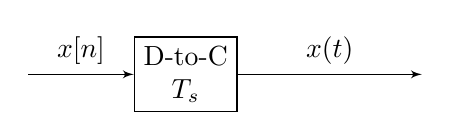
\begin{tikzpicture}[every text node part/.style={align=center},node distance=3cm,auto,>=latex']
      \node [int] (a) {D-to-C \\ $T_s$};
      \node (b) [left of=a,node distance=2cm, coordinate] {a};
      %    \node (c) [below=a,node distance=3cm] {a};

      %\node [int, pin={[init]above:$p_0$}] (c) [right of=a] {$\frac{1}{s}$};
      \node [coordinate] (end) [right of=a, node distance=3cm]{};
      \path[->] (b) edge node {$x[n]$} (a);
      \draw[->] (a) edge node {$x(t)$} (end) ;
    \end{tikzpicture}
    % }
  \end{center}
  \caption{A Discrete-time to Continuous-time (D-to-C) converter.}
\end{marginfigure}

Reconstruction involves transforming a discrete-time signal into a continuous-time signal. 
This type of operation is done, e.g., when
translating an audio signal into air pressure variations to create sound.

In order to convert a discrete-time signal into a continuous-time signal, some form 
of interpolation is needed in order to fill in the space between the samples. 
This is the function of a reconstruction filter, or a discrete-time to continuous-time (D-to-C) system:
\begin{equation}
  x(t) = \mathcal{R}\{x[n]\}\,\,.
\end{equation}
The ingredients that are needed to reconstruct the signal are the samples $x[n]$, information about the
sampling rate $T_s=1/f_s$, and information about the Nyquist zone that the signal is within.

This is equivalent to knowing the true values of the discrete-time frequencies $\hat{\omega}$ of all the discretized spectral
components, i.e., being able to rule out all the aliases using a priori knowledge of the frequency band that the signal lies in.

There are several ways to perform this reconstruction. If the analytical form of the signal is 
known, as in the case of a sinusoid, the signal can be generated analytically based on the 
phase and amplitude of the signal. In other cases, some form of interpolation is needed.

\subsection{Interpolation filters}
In this section, we'll only cover reconstruction of oversampled signals\footnote{It is possible to derive interpolation filters
  for reconstruction of undersampled signals in the same way, but this is beyond the scope of this course.} that satisfy
the Nyquist-Shannon sampling criterion $f_s > 2f_{\mathrm{max}}$, i.e., 
the spectral components of the signal are between $-f_s/2 < f < f_s/2$.

We can convert a discrete-time signal into a continuous-time signal using an interpolation filter of the form:
\begin{equation}
  x(t) = \sum_{n=-\infty}^{\infty} x[n]p(t-nT_s)\,\,.
\end{equation}
Theoretically, this interpolation filter can use the discrete-time samples to obtain the continuous-time reconstruction.
\begin{marginfigure}
  \begin{center}
    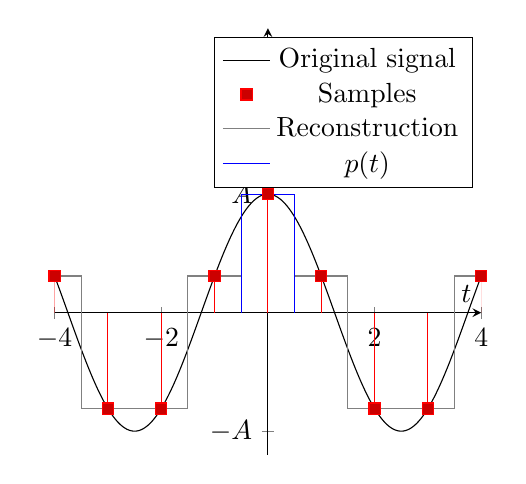
\begin{tikzpicture}
      \begin{axis}[domain=-5:5,
          width=7cm,height=7cm,ymin=-1.2,xmin=-4,ymax=2.4,xmax=4,
          ytick={-1,1},
          yticklabels={$-A$, $A$},
          xlabel=$t$, axis lines = center]
        \addplot[samples=400]{cos(deg(2.0*3.1415*0.2*x))};
        \addplot+[ycomb,samples=11]{cos(deg(2.0*3.1415*0.2*x))};
        \addplot[mark=none,color=gray] plot coordinates {(-4.5,0.30901699) (-3.5,0.30901699) (-3.5,-0.80901699) (-2.5,-0.80901699) (-2.5,-0.80901699) (-1.5,-0.80901699) (-1.5,0.30901699) (-0.5,0.30901699) (-0.5,1.) (0.5,1.) (0.5,0.30901699) (1.5,0.30901699) (1.5,-0.80901699) (2.5,-0.80901699) (2.5,-0.80901699) (3.5,-0.80901699)  (3.5,0.30901699) (4.5,0.30901699)};

        \addplot[mark=none,color=blue] plot coordinates {(-0.5,0.0) (-0.5,1.0) (0.5,1.0) (0.5,0)};                             %  \addplot[samples=100,domain=-0.5:0.5,color=blue]{1};

        \legend{Original signal,Samples, Reconstruction, $p(t)$}
      \end{axis}
    \end{tikzpicture}
  \end{center}
  \caption{Zero-order hold interpolation.}
  \label{fig:z-o-hold}
\end{marginfigure}

\newthought{The zero-order hold filter} is the simplest interpolation filter. 
It obtains a constant value for the duration of a sample.
The filter in this case has the following mathematical definition:
\begin{equation}
  p(t) = \left\{
  \begin{array}{rcr}
    1 & \mathrm{when}      & -\frac{T_s}{2} < t \le \frac{T_s}{2} \\
    0 & \mathrm{otherwise} &                                      \\
  \end{array}
  \right\} \,\,.
\end{equation}
The generated continuous-time signal looks like the one shown in Figure \ref{fig:z-o-hold}.

\begin{marginfigure}
  \begin{center}
    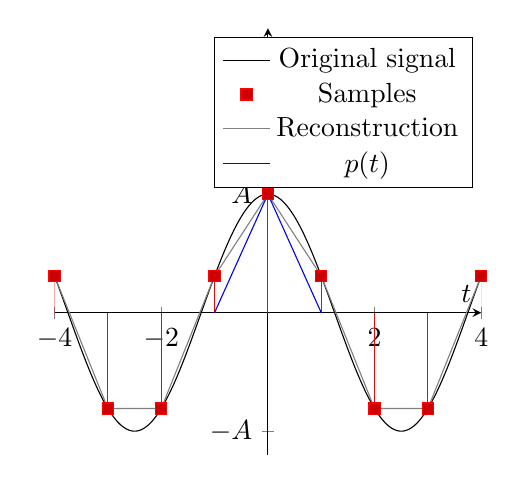
\begin{tikzpicture}
      \begin{axis}[domain=-5:5,
          width=7cm,height=7cm,ymin=-1.2,xmin=-4,ymax=2.4,xmax=4,
          ytick={-1,1},
          yticklabels={$-A$, $A$},
          xlabel=$t$, axis lines = center]
        \addplot[samples=400]{cos(deg(2.0*3.1415*0.2*x))};
        \addplot+[ycomb,samples=11]{cos(deg(2.0*3.1415*0.2*x))};
        \addplot[mark=none,color=gray] plot coordinates {(-4,0.30901699) (-3,-0.80901699) (-2,-0.80901699) (-1,0.30901699) (0.0,1.)  (1,0.30901699) (2,-0.80901699) (3,-0.80901699) (4,0.30901699) };
        \addplot[samples=100,domain=-1:1,color=blue]{1-abs(x)};

        \legend{Original signal,Samples, Reconstruction, $p(t)$}
      \end{axis}
    \end{tikzpicture}
  \end{center}
  \caption{Linear interpolation filter.}
  \label{fig:lin_int_filter}
\end{marginfigure}

The zero-order hold filter only needs one sample at a time. However, the continuous-time signal has large steps.
The zero-order hold filter approaches the continuous-time signal only when $T_s\rightarrow 0$ -- i.e., 
when the sample rate is infinitely large.

\newthought{A Linear interpolation filter} is defined as follows:
\begin{equation}
  p(t) = \left\{
  \begin{array}{rcr}
    1-\frac{|t|}{T_s} & \mathrm{when}      & -T_s < t < T_s \\
    0                 & \mathrm{otherwise} &                \\
  \end{array}
  \right\} \,\,.
\end{equation}
It applies a linear interpolation between two consecutive samples. The generated continuous-time signal 
is depicted in Figure \ref{fig:lin_int_filter}.

\newthought{The ideal reconstruction filter} is based on the
Shannon-Nyquist sampling theorem. It guarantees theoretically that a continuous-time real-valued signal 
can be perfectly reconstructed from discrete-time samples for
signals occupying the band $-f_s/2 < f < f_s/2$, if $f_s > 2f_{\mathrm{max}}$.
Here $f_{\mathrm{max}}$ is the maximum frequency component within the signal. We'll prove this 
theorem at the end of this chapter.

In order to reconstruct the signal perfectly in a mathematical sense, an ideal 
reconstruction filter must be used.
Something approximately resembling a truncated or tapered version of an ideal reconstruction filter is 
typically used in real world applications.

The form of this ideal reconstruction filter can be derived from the inverse Fourier transform of a 
rectangular shaped window that in frequency domain is an ideal low pass filter:
\begin{equation}
  P(\omega) = \left\{
  \begin{array}{rcr}
    T_s & \mathrm{when}      & |\omega| \le \pi f_s \\
    0   & \mathrm{otherwise} &                      \\
  \end{array}
  \right. \,\,.
\end{equation}
\begin{marginfigure}
  \begin{center}
    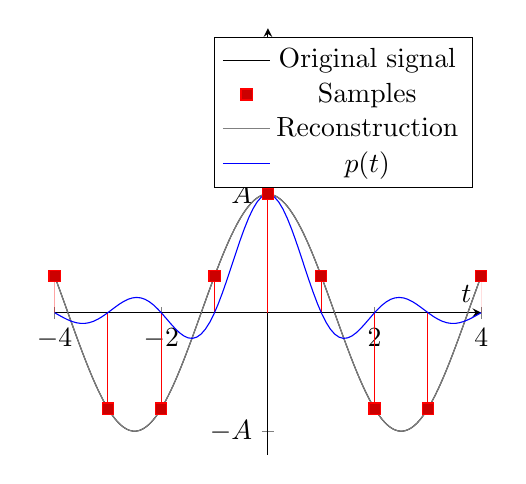
\begin{tikzpicture}
      \begin{axis}[domain=-5:5,
          width=7cm,height=7cm,ymin=-1.2,xmin=-4,ymax=2.4,xmax=4,
          ytick={-1,1},
          yticklabels={$-A$, $A$},
          xlabel=$t$, axis lines = center]
        \addplot[samples=400]{cos(deg(2.0*3.1415*0.2*x))};
        \addplot+[ycomb,samples=11]{cos(deg(2.0*3.1415*0.2*x))};
        \addplot[samples=400,mark=none,color=gray]{cos(deg(2.0*3.1415*0.2*x))};
        \addplot[samples=100,domain=-4:4,color=blue]{sin(deg((3.14)*(x+0.0000001)))/(3.14*(x+0.000001))};

        \legend{Original signal,Samples, Reconstruction,$p(t)$}
      \end{axis}
    \end{tikzpicture}
  \end{center}
  \caption{Ideal reconstruction filter.}
\end{marginfigure}
Here $P(\omega)$ is the Fourier transform of the reconstruction
filter, $\omega$ is angular frequency. The resulting ``ideal''
reconstruction filter is:
\begin{align}
  p(t) & =\frac{1}{2\pi}\int_{-\infty}^{\infty} P(\omega)e^{i\omega t}d\omega \\
       & = \frac{T_s}{\pi t}\sin\left(\frac{\pi}{T_s}t\right)\,\,.
\end{align}
This filter is infinitely long, which implies that all samples need to be used in order for the 
reconstructed signal to be mathematically perfect.

\if 0
  Similar reconstruction filters exists for other Nyquist zones, which allow perfect 
  reconstruction of undersampled signals, which satisfy the Shannon-Nyquist sampling criterion. 
  Such filters use ideal reconstruction filters that can be derived from idealized band-pass filters:
  \begin{equation}
    P(\omega) = \left\{
    \begin{array}{rcr}
      T_s & \mathrm{when}      & k\omega_s/2 \le |\omega| < (k+1)\omega_s/2 \\
      0   & \mathrm{otherwise} &                                            \\
    \end{array}
    \right\} \,\,.
  \end{equation}
  Here $k$ specifies the Nyquist zone for which the signal is to be reconstructed in.
\fi

\section{Shannon's sampling theorem}
\begin{marginfigure}
  \begin{center}
    \includegraphics[width=\textwidth]{ch09/figures/shannon_mouse.png}
  \end{center}
  \caption{Claude Elwood Shannon. Photo: Bell Labs.}
\end{marginfigure}

Shannon's sampling theorem is a fundamental theorem in information theory and signal 
processing\sidenote{This theorem was discovered by Edmund Whittaker 33 years before Claude Shannon, 
and thus sometimes the sampling theory is called the Whittaker-Shannon sampling theorem.\cite{whittaker1915xviii,shannon1948mathematical}}. 
It relates the sample-rate of a discrete-time signal to the bandwidth of a continuous-time signal in frequency domain.
The full form of the theory is not just: ``use a sample-rate that is at least twice as large as the largest 
frequency component in the continuous-time signal''. There are other solutions, which also guarantee that no 
information about the signal is lost.
The most general way to investigate if information is lost when discretizing a signal is to explore 
the relationship between the Fourier transform of the signal, and the Fourier transform of the discretized signal.

We will assume that information is contained in the shape of the signal $x(t)$. 
This signal is assumed to be band-limited in frequency domain.
This means that the spectrum is zero valued outside a certain range of frequencies: 
$\hat{x}(\omega) = 0$ when $\omega < \omega_{\mathrm{min}}$ or $\omega > \omega_{\mathrm{max}}$.

Is it possible to form a discrete-time signal $x[n]$ from $x(t)$ in such a way that $x[n]$ contains sufficient information to
allow us to perfectly reconstruct $x(t)$? In other words, can we perfectly reconstruct a continuous-time signal $x(t)$ from
its discrete-time representation? This is the question that Shannon studied, and his sampling theorem provides an answer to.

\subsection{Sampling}
\begin{marginfigure}[3cm]
  \begin{center}
    \includegraphics[width=\textwidth]{ch09/figures/whittaker.jpg}
  \end{center}
  \caption{Sir Eduard Whittaker. Photo: National Portrait Gallery.}
\end{marginfigure}

In the idealized case, sampling of a signal is selection of samples from a continuous-time signal:
\begin{equation}
  x[n] = x(nT_s)
\end{equation}
where $T_s$ is the sample spacing. This is the inverse of the sample-rate $T_s = f_s^{-1}$. 
We can express this sampling process using the Dirac delta function, 
where a delayed Dirac delta ``samples'' the value of the signal $x(t)$ at time $nT_s$:
\begin{equation}
  x[n] = \int_{-\infty}^{\infty}x(t)\delta(t-nT_s)dt = x(nT_s).
\end{equation}
We can use a train of Dirac delta functions (Dirac comb)
\begin{equation}
  s(t) = \sum_{n=-\infty}^{\infty}\delta(t-nT_s),
\end{equation}
to represent the sampled signal in continuous-time:
\begin{align}
  x_s(t) & = x(t) s(t)                                     \\
         & = x(t) \sum_{n=-\infty}^{\infty} \delta(t-nT_s) \\
         & = \sum_{n=-\infty}^{\infty} x[n]\delta(t-nT_s)
\end{align}
The sampled signal $x_s(t)$ is a continuous-time signal, which has the same information 
content as the array of samples $x[n]$. This means that $x_s(t)$ can be formed just by 
knowledge of the discrete-time signal $x[n]$.

\subsection{Fourier series representation for Dirac comb}
The Dirac comb
\begin{equation}
  s(t) = \sum_{k=-\infty}^{\infty} \delta(t-kT_s),
\end{equation}
is a periodic function with period $T_s$. Therefore, it is possible to express it as a Fourier series:
\begin{equation}
  s(t) = \sum_{k=-\infty}^{\infty} c_k e^{i\frac{2\pi}{T_s}kt}.
\end{equation}
The coefficients of the Fourier series can be obtained using the Fourier series synthesis equation, 
by integrating over one period of the function:
\begin{align}
  c_k & = \frac{1}{T_s}\int_{-T_s/2}^{T_s/2} \left[\sum_{n=-\infty}^{\infty} \delta(t-nT_s) \right] e^{-i\frac{2\pi}{T_s}kt}dt \\
      & =\frac{1}{T_s}\int_{-T_s/2}^{T_s/2} \delta(t)  e^{-i\frac{2\pi}{T_s}kt}dt                                              \\
      & =\frac{1}{T_s}e^{-i\cdot 0}                                                                                            \\
      & =\frac{1}{T_s}
\end{align}
We also note that $2\pi/T_s = \omega_s$, which is the sample-rate expressed as an angular frequency. 
The Fourier series representation of the Dirac-comb is therefore:
\begin{equation}
  s(t) = \frac{1}{T_s}\sum_{k=-\infty}^{\infty} e^{i k \omega_s t}.
\end{equation}
This Fourier series representation can now be substituted to represent the sampling operation as:
\begin{align}
  x_s(t) & = x(t)s(t)                                                                     \\
         & = x(t)  \left(\frac{1}{T_s}\sum_{k=-\infty}^{\infty} e^{i k \omega_s t}\right)
\end{align}

\subsection{Spectral representation of $x_s(t)$ and $x(t)$}
We then Fourier transform $x_s(t)$ to study the relationship between the sample-rate and 
the bandwidth of the signal.
We use the property that multiplication in time domain is convolution in frequency domain. 
The Fourier transform of $x(t)$ is $\hat{x}(\omega)$.
The Fourier transform of $s(t)$ is $\hat{s}(\omega)$. We also make use of the fact that the 
Fourier transform of $e^{i k \omega_s t}$ is $2\pi\delta(\omega-k\omega_s)$:
\begin{align}
  \hat{x}_s(\omega) & = \frac{1}{2\pi}  \hat{x}(\omega)*\hat{s}(\omega)\label{eq:xs_spec}                                                                                            \\
                    & = \frac{1}{2\pi}\int_{-\infty}^{\infty}\hat{x}(\omega') \hat{s}(\omega-\omega')d\omega'                                                                        \\
                    & = \frac{1}{2\pi} \int_{-\infty}^{\infty} \hat{x}(\omega')\left(\frac{1}{T_s}\sum_{k=-\infty}^{\infty} 2\pi \delta(\omega- k\omega_s - \omega')\right) d\omega' \\
                    & = \frac{1}{T_s} \sum_{k=-\infty}^{\infty}\int_{-\infty}^{\infty} \hat{x}(\omega')\delta(\omega - k\omega_s - \omega') d\omega'                                 \\
                    & = \frac{1}{T_s} \sum_{k=-\infty}^{\infty} \hat{x}(\omega-k\omega_s).
\end{align}
In other words, the Fourier transform of the sampled function $x_s(t)$ is infinitely 
many copies of $\hat{x}(\omega)$, each shifted by $k\omega_s$ and scaled in 
amplitude by $\frac{1}{T_s}$.

We illustrate this using the following two figures. The first one depicts the magnitude 
spectrum of the original continuous-time signal $x(t)$:
\begin{center}
  \begin{tikzpicture}
    \begin{axis}[width=15cm,height=5cm,ymin=0,ymax=3,
        xmin=-11,xmax=11,
        xlabel={$\omega$},
        ylabel={$|\hat{x}(\omega)|$},
        axis x line=center,
        axis y line=center,
        yticklabels={,,,},
        xtick={-6,-3,3,6},
        xticklabels={$-\omega_s$,$-\omega_s/2$,$\omega_s/2$,$\omega_s$}
      ]
      \addplot[mark=none,color=blue] plot coordinates {(-10,0.0) (-1,0) (-0.8,2*0.8) (-0.2,2*1) (0,0) (0.2,2*1) (0.8,2*0.8) (1,0)  (7,0)};

    \end{axis}
  \end{tikzpicture}
\end{center}
The sampled signal $x_s(t)$ has a periodic spectrum $\hat{x}_s(\omega)
  = \hat{x}_s(\omega+k\omega_s)$, which has a period $\omega_s$:
\begin{center}
  \begin{tikzpicture}
    \begin{axis}[width=15cm,height=5cm,ymin=0,ymax=3,
        xmin=-11,xmax=11,
        xlabel={$\omega$},
        ylabel={$|\hat{x}_s(\omega)|$},
        axis x line=center,
        axis y line=center,
        yticklabels={,,,},
        xtick={-6,-3,3,6},
        xticklabels={$-\omega_s$,$-\omega_s/2$,$\omega_s/2$,$\omega_s$}
      ]
      \addplot[mark=none,color=blue] plot coordinates {(-10,0.0) (-7,0) (-6.8,2*0.8) (-6.2,2*1) (-6,0) (-5.8,2*1) (-5.2,2*0.8) (-5,0) (-1,0) (-0.8,2*0.8) (-0.2,2*1) (0,0) (0.2,2*1) (0.8,2*0.8) (1,0)  (5,0) (5.2,2*0.8) (5.8,2*1) (6,0) (6.2,2*1) (6.8,2*0.8) (7,0)};
      \draw node at (axis cs:-9,0.5) {$\cdots$};
      \draw node at (axis cs:9,0.5) {$\cdots$};
    \end{axis}
  \end{tikzpicture}
\end{center}
This probably already provides some idea of what the sample-rate should be, in order to 
avoid losing information. The most straightforward answer is that if the spectrum of the 
original signal $\hat{x}(\omega)$ is confined within the limits of $\pm \omega_s/2$, 
then no overlap between the different copies of $\hat{x}(\omega)$ occurs.

There are other solutions that avoid aliasing for real-valued signals. The original 
signal $\hat{x}(\omega)$ might also be confined in frequency to one of 
the intervals $n \omega_s/2 \le |\omega| < (n+1)\omega_s/2$ with $n\in\mathbb{Z}$.
This property is widely used when sampling radio signals that are at a much higher 
frequency than the sample rate. This type of sampling strategy is called undersampling.

\subsection{Aliasing}
If the different copies of $\hat{x}(\omega)$ in $\hat{x}_s(\omega)$ overlap, then 
aliasing occurs. For example, if the spectrum of $\hat{x}(\omega)$ extends over the 
limits $\pm \omega_s/2$, then there are regions where $\hat{x}_s(\omega)$ is occupied 
by two or more spectral components of $\hat{x}(\omega)$ at the same time.

If the frequency extent of the original signal $\hat{x}(\omega)$ is larger than $\omega_s$, 
then aliasing occurs as shown below:
\begin{center}
  \begin{tikzpicture}
    \begin{axis}[width=15cm,height=5cm,ymin=0,ymax=3,
        xmin=-11,xmax=11,
        xlabel={$\omega$},
        ylabel={},
        axis x line=center,
        axis y line=center,
        yticklabels={,,,},
        xtick={-6,-3,3,6},
        xticklabels={$-\omega_s$,$-\omega_s/2$,$\omega_s/2$,$\omega_s$}
      ]
      \addplot[mark=none,color=blue] plot coordinates {(-10,0.0) (-9.5,0) (-6.8,2*0.8) (-6.2,2*1) (-6,0) (-5.8,2*1) (-5.2,2*0.8) (-2.5,0) (-3.5,0) (-0.8,2*0.8) (-0.2,2*1) (0,0) (0.2,2*1) (0.8,2*0.8) (3.5,0)  (2.5,0) (5.2,2*0.8) (5.8,2*1) (6,0) (6.2,2*1) (6.8,2*0.8) (9.5,0) (10,0) } ;
      \addlegendentry{$\hat{s}(\omega + k\omega_s)$}
      \addplot[mark=none,color=red] plot coordinates {(-9.5,0.5775) (-8.5,0.5775) (-6.8,2*0.8) (-6.2,2*1) (-6,0) (-5.8,2*1) (-5.2,2*0.8) (-3.5,0.5775) (-2.5,0.5775) (-0.8,2*0.8) (-0.2,2*1) (0,0) (0.2,2*1) (0.8,2*0.8) (2.5,0.5775)  (3.5,0.5775) (5.2,2*0.8) (5.8,2*1) (6,0) (6.2,2*1) (6.8,2*0.8) (8.5,0.5775) (9.5,0.5775)};
      \addlegendentry{$\hat{x}_s(\omega)$}
      \draw node at (axis cs:-10,0.5) {$\cdots$};
      \draw node at (axis cs:10,0.5) {$\cdots$};

      %    \addplot[mark=none,color=blue] plot coordinates {(-10,0.0) (-7,0) (-6.8,2*0.8) (-6.2,2*1) (-6,0) (-5.8,2*1) (-5.2,2*0.8) (-5,0) (-1,0) (-0.8,2*0.8) (-0.2,2*1) (0,0) (0.2,2*1) (0.8,2*0.8) (1,0)  (5,0) (5.2,2*0.8) (5.8,2*1) (6,0) (6.2,2*1) (6.8,2*0.8) (7,0) } ;
    \end{axis}
  \end{tikzpicture}
\end{center}
In this case, positive and negative frequency components of the original spectrum $\hat{x}_s(\omega)$ 
overlap and are added together when $|\omega| > \omega_s/2$,
making it impossible to determine what the original value of $\hat{x}(\omega)$ is within the overlapping region.

\subsection{Complex-valued signal}
For a complex-valued signal $x(t)\in \mathbb{C}$, a sufficient condition for avoiding $\hat{x}(\omega)$ 
overlapping with itself in $\hat{x}_s(\omega)$ (aliasing) is that $\omega_s > \omega_{\mathrm{max}}-\omega_{\mathrm{min}}$.

Aliasing with complex signals is illustrated with the following plots. Consider a signal, which spans 
between frequencies $0.11\omega_s$ and $1.1\omega_s$.
In this case, the signal crosses $\omega_s/2$, which violates aliasing rules for real-valued signals. 
However, $\omega_s > \omega_{\mathrm{max}}-\omega_{\mathrm{min}}$.
\begin{center}
  \begin{tikzpicture}
    \begin{axis}[width=15cm,height=5cm,ymin=0,ymax=3,
        xmin=-11,xmax=11,
        xlabel={$\omega$},
        ylabel={$\hat{x}(\omega)\in \mathbb{C}$},
        axis x line=center,
        axis y line=center,
        yticklabels={,,,},
        xtick={-6,-3,3,6},
        xticklabels={$-\omega_s$,$-\omega_s/2$,$\omega_s/2$,$\omega_s$}
      ]
      \addplot[mark=none,color=blue] plot coordinates {(-10,0) (1.2,0) (2,0.5) (6,1) (7,0) (10,0) } ;

    \end{axis}
  \end{tikzpicture}
\end{center}
The spectrum of the sampled signal $x_s(t)$ has a periodic spectrum
$\hat{x}_s(\omega) = \hat{x}_s(\omega+k\omega_s)$. Notice that there
is no overlap between the copies of the spectrum:
\begin{center}
  \begin{tikzpicture}
    \begin{axis}[width=15cm,height=5cm,ymin=0,ymax=3,
        xmin=-11,xmax=11,
        xlabel={$\omega$},
        ylabel={$|\hat{x}_s(\omega)|$},
        axis x line=center,
        axis y line=center,
        yticklabels={,,,},
        xtick={-6,-3,3,6},
        xticklabels={$-\omega_s$,$-\omega_s/2$,$\omega_s/2$,$\omega_s$}
      ]
      \addplot[mark=none,color=blue] plot coordinates {(-10,0) (1.2,0) (2,0.5) (6,1) (7,0) (10,0) } ;
      \addplot[mark=none,color=blue] plot coordinates {(-10,0) (1.2+6,0) (2+6,0.5) (6+6,1) (7+6,0) (10+6,0) } ;

      \addplot[mark=none,color=blue] plot coordinates {(-10,0) (1.2-6,0) (2-6,0.5) (6-6,1) (7-6,0) (10-6,0) } ;
      \addplot[mark=none,color=blue] plot coordinates {(-10-12,0) (1.2-12,0) (2-12,0.5) (6-12,1) (7-12,0) (10-12,0) } ;

      \draw node at (axis cs:-9,0.5) {$\cdots$};
      \draw node at (axis cs:9,0.5) {$\cdots$};

      %    \addplot[mark=none,color=blue] plot coordinates {(-10,0.0) (-7,0) (-6.8,2*0.8) (-6.2,2*1) (-6,0) (-5.8,2*1) (-5.2,2*0.8) (-5,0) (-1,0) (-0.8,2*0.8) (-0.2,2*1) (0,0) (0.2,2*1) (0.8,2*0.8) (1,0)  (5,0) (5.2,2*0.8) (5.8,2*1) (6,0) (6.2,2*1) (6.8,2*0.8) (7,0) } ;
    \end{axis}
  \end{tikzpicture}
\end{center}
This means that the values of $\hat{x}_s(\omega)$ between, e.g., $0.11\omega_s$ and $1.1\omega_s$ fully 
determine the frequency domain representation of the original signal $\hat{x}(\omega)$.

\subsection{Sampling criteria}
The Shannon-Nyquist sampling theorem requires that it should be possible to reconstruct $\hat{x}(\omega)$ from
$\hat{x}_s(\omega)$. The commonly described criterion that requires the sample-rate to be higher than twice the 
largest frequency component of the signal:
\begin{equation}
  f_s > 2 f_\mathrm{max}
\end{equation}
is just one possible solution, which assumes that the spectral components within the 
original signal $\hat{x}(\omega)$ are confined to $|f| < f_s/2$. As we discussed above, 
complex-valued signals and under sampled signals result in different sampling criteria.

\subsection{Reconstruction}
This reconstruction strategy only applies to a real-valued signal $x(t) \in \mathbb{R}$ 
within the principal spectrum.
It should be easy to determine how to create a reconstruction filter for, e.g., a 
complex-valued signal occupying the band $\omega \in [\omega_{\mathrm{min}},\omega_{\mathrm{max}}]$ 
after following this derivation.

In order to reconstruct signal $x(t)$ from $x[n]$, we first form $x_s(t)$ using $x[n]$:
\begin{equation}
  x_s(t) = \sum_{n=-\infty}^{\infty} x[n]\delta(t-n T_s)
\end{equation}
We then use an ideal low-pass filter specified in frequency domain as:
\begin{equation}
  \Hiw = \left\{ \begin{array}{cc}
    T_s & |\omega| \le \frac{\omega_s}{2} \\
    0   & \mathrm{otherwise}
  \end{array}
  \right.
\end{equation}
When we apply this filter $\hat{x}_s(\omega)$ to reconstruct $\hat{x}(\omega)$:
\begin{align}
  \Hiw \hat{x}_s(\omega) & = \Hiw\frac{1}{T_s} \sum_{k=-\infty}^{\infty} \hat{x} (\omega-k\omega_s) \\
                         & = \hat{x}(\omega) \qed
\end{align}
This operation is shown in the Figure below:
\begin{center}
  \begin{tikzpicture}
    \begin{axis}[width=15cm,height=5cm,ymin=0,ymax=3,
        xmin=-11,xmax=11,
        xlabel={$\omega$},
        ylabel={$|\hat{x}_s(\omega)|$},
        axis x line=center,
        axis y line=center,
        yticklabels={,,,},
        xtick={-6,-3,3,6},
        xticklabels={$-\omega_s$,$-\omega_s/2$,$\omega_s/2$,$\omega_s$}
      ]
      \addplot[mark=none,color=blue] plot coordinates {(-10,0.0) (-9.0,0) (-6.8,2*0.8) (-6.2,2*1) (-6,0) (-5.8,2*1) (-5.2,2*0.8) (-3,0) (-3,0) (-0.8,2*0.8) (-0.2,2*1) (0,0) (0.2,2*1) (0.8,2*0.8) (3,0)  (3,0) (5.2,2*0.8) (5.8,2*1) (6,0) (6.2,2*1) (6.8,2*0.8) (9,0) (10,0) } ;
      \draw node at (axis cs:-10,0.5) {$\cdots$};
      \draw node at (axis cs:10,0.5) {$\cdots$};
      \draw node at (axis cs:3.5,2.5) {$\Hiw$};
      \addplot[mark=none,color=red] plot coordinates {(-10,0.0) (-3,0) (-3,2.2) (3,2.2) (3,0) (10,0) } ;

      %    \addplot[mark=none,color=blue] plot coordinates {(-10,0.0) (-7,0) (-6.8,2*0.8) (-6.2,2*1) (-6,0) (-5.8,2*1) (-5.2,2*0.8) (-5,0) (-1,0) (-0.8,2*0.8) (-0.2,2*1) (0,0) (0.2,2*1) (0.8,2*0.8) (1,0)  (5,0) (5.2,2*0.8) (5.8,2*1) (6,0) (6.2,2*1) (6.8,2*0.8) (7,0) } ;
    \end{axis}
  \end{tikzpicture}
  \begin{tikzpicture}
    \begin{axis}[width=15cm,height=5cm,ymin=0,ymax=3,
        xmin=-11,xmax=11,
        xlabel={$\omega$},
        ylabel={$|\hat{x}(\omega)|$},
        axis x line=center,
        axis y line=center,
        yticklabels={,,,},
        xtick={-6,-3,3,6},
        xticklabels={$-\omega_s$,$-\omega_s/2$,$\omega_s/2$,$\omega_s$}
      ]
      \addplot[mark=none,color=blue] plot coordinates {(-10,0.0)  (-3,0) (-0.8,2*0.8) (-0.2,2*1) (0,0) (0.2,2*1) (0.8,2*0.8) (3,0)   (10,0) } ;

      ;
    \end{axis}
  \end{tikzpicture}
\end{center}
This is in essence the proof of Shannon's sampling theorem. To obtain $x(t)$, 
one can use an inverse Fourier transform:
\begin{equation}
  x(t) = \frac{1}{2\pi}\int_{-\infty}^{\infty} \hat{x}(\omega) e^{i\omega t}d\omega.
\end{equation}
If $\hat{x}_s(\omega)$ contains overlapping copies of $\hat{x}(\omega)$, then the original 
spectrum $\hat{x}(\omega)$, and therefore the original signal $x(t)$, cannot be reconstructed.

For a complex-valued signal, we would need to apply an ideal band-pass filter, which only 
retains signals between $\omega_{\mathrm{min}}$ and
$\omega_{\mathrm{max}}$, instead of the ideal low-pass filter. The same applies to an undersampled signal.

\subsection{Ideal reconstruction filter}
Recall, from the beginning of this course, that we introduced the ideal reconstruction filter without deriving it. 
Now we can derive it. It is the inverse Fourier transform of the ideal low-pass filter
\begin{equation}
  \Hiw = \left\{ \begin{array}{cc}
    T_s & |\omega| \le \frac{\omega_s}{2} \\
    0   & \mathrm{otherwise}
  \end{array}
  \right.
\end{equation}
which is
\begin{align}
  h(t) & = \frac{1}{2\pi}\int_{-\infty}^{\infty} \Hiw e^{i\omega t}d\omega                             \\
       & = \frac{1}{2\pi} \int_{-\omega_s/2}^{\omega_s/2} T_s e^{i\omega t}d\omega                     \\
       & = \frac{T_s}{2 \pi}\left. \frac{e^{i\omega t}}{it} \right|_{\omega=-\omega_s/2}^{\omega_s/2}  \\
       & = \frac{T_s}{2 t \pi i}\left( e^{i\frac{\omega_s}{2} t}  - e^{-i\frac{\omega_s}{2} t} \right) \\
       & = \frac{T_s}{\pi t} \sin(\frac{\omega_s}{2}t)                                                 
\end{align}
Keeping in mind that $\omega_s/2 = \pi/T_s$ we obtain the familiar result:
\begin{equation}
  \boxed{
    h(t) = \frac{T_s}{\pi t}\sin(\frac{\pi}{T_s}t)
  }
\end{equation}
When applying this reconstruction filter in time domain, one convolves the sampled signal to obtain the 
reconstructed continuous-time signal:
\begin{align}
  x(t) & = h(t)*x_s(t)                                                                                            \\
       & = \int_{-\infty}^{\infty} x_s(\tau)h(t-\tau)d\tau                                                        \\
       & = \int_{-\infty}^{\infty}\left( \sum_{n=-\infty}^{\infty} x[n] \delta(\tau-n T_s)\right) h(t-\tau) d\tau \\
       & = \sum_{n=-\infty}^{\infty} x[n] \int_{-\infty}^{\infty} \delta(\tau-nT_s) h(t-\tau)d\tau                \\
       & = \sum_{n=-\infty}^{\infty} x[n] \frac{\sin(\frac{\pi}{T_s}(t-n T_s))}{\frac{\pi}{T_s}(t-nT_s)}.
\end{align}
This reconstruction formula now perfectly reproduces $x(t)$ from
samples $x[n]$, provided that $\omega_s \ge 2\omega_{\mathrm{max}}$.

For an undersampled real-valued signal, or a complex-valued band limited signal, the ideal reconstruction 
filter would be different. In this case, it would correspond to the impulse response of an ideal band-pass filter.

\input{ch09/exercises9}
 \ifSpExerciseSol
 \input{ch09/solutions9}
 \fi
\fi

\ifSpLTI
\chapter{Linear Time-invariant Systems}
\index{Linear time-invariant systems}{Linear time-invariant systems}
(LTI) are an important class of systems that can be analyzed easily in frequency domain.
An LTI system is equivalent to \emph{\index{convolution}{convolution}} of the \emph{impulse response} of the system.
The focus of this chapter is to learn more about what these concepts are.

\section{Example: Running average filter}
Here's an example of a discrete-time system that you might use to smooth a noisy signal:
\begin{equation}
  y[n] = \frac{1}{15}\sum_{k=-7}^{7} x[n-k]\,\,.
  \label{eq:running_mean}
\end{equation}
What does this system do? It averages together 15 neighboring values of the input signal $x[n]$.
Figure \ref{fig:avg_filter} shows a demonstration of this system in action.
The blue line indicates a noisy input signal $x[n]$, and the orange line depicts the output
$y[n]$ of the running mean filter given in Equation \ref{eq:running_mean}.
As you might expect, the output of the system is a smoother version of the input signal.
\begin{figure}
  \begin{center}
    \includegraphics[width=\textwidth]{code/016_smoothing/smoothing.png}
  \end{center}
  \caption{A running average filter is often used to smooth a noisy
    signal. You can find the Python code used to produce this example
    in \texttt{016\_smoothing/smoothing.py}.}
  \label{fig:avg_filter}
\end{figure}

\section{Finite impulse response filter}
\begin{marginfigure}

  \begin{center}
    \begin{tikzpicture}[node distance=3cm,auto,>=latex']
      \node [int] (a) {LTI};
      \node (b) [left of=a, coordinate] {a};
      %    \node (c) [below=a,node distance=3cm] {a};

      %\node [int, pin={[init]above:$p_0$}] (c) [right of=a] {$\frac{1}{s}$};
      \node [coordinate] (end) [right of=a]{};
      \path[->] (b) edge node {$x[n]$} (a);
      \path[->] (b) edge node [below]{$\delta[n]$} (a);

      %\path[->] (a) edge node {$v$} (c);
      \draw[->] (a) edge node {$y[n]$} (end) ;
      \draw[->] (a) edge node [below]{$h[n]$} (end) ;

    \end{tikzpicture}
  \end{center}
  \caption{Discrete-time LTI systems are characterized by an impulse response $h[n]$, 
  which is the response of the LTI system to a unit impulse signal.}
\end{marginfigure}

The previous system shown in Equation \ref{eq:running_mean} is a special case of a 
more general type of discrete-time LTI system,
known as a Finite Impulse Response (FIR) filter. This type of signal is often 
used in digital signal processing.
An FIR filter is defined as follows:
\begin{equation}
  \boxed{
    y[n] = \sum_{k=-M}^{N} b_k x[n-k]\,\,.
  }
  \label{eq:fir_filter}
\end{equation}
The coefficients $b_k \in \mathbb{C}$ here are constant valued coefficients. 
As the name implies, there is a finite number of non-zero coefficients $b_k$.
In the case of the running average filter in Equation \ref{eq:running_mean}, 
there would be 15 coefficients, which are all $b_k=1/15$.

\section{General discrete-time LTI system}
What if we allow there to be infinitely many coefficients for the system given 
in Equation \ref{eq:fir_filter}? We get the following:
\begin{equation}
  y[n] = \sum_{k=-\infty}^{\infty} b_k x[n-k] = \sum_{k=-\infty}^{\infty} b[k] x[n-k]\,\,.
\end{equation}
This turns out to be the general representation for arbitrary discrete-time LTI systems! 
In this case, it makes sense to think of the infinitely many coefficients $b_k$ as a signal $b[k]$.

For discrete-time LTI systems in general, the output of a system is given by a discrete-time 
convolution sum of the input signal $x[n]$ with an impulse response $h[n]$:

\begin{marginfigure}
  \begin{center}
    \begin{tikzpicture}
      \begin{axis}[width=7cm,height=4cm,ymin=0,xmin=-10,ymax=0.1,xmax=12,
          xtick={-10,-7,0,7,10},
          ytick={0,1,2,3},
          ytick={0,0.0667},
          yticklabel={,,},
          ylabel={$h[n]$},
          xlabel={$n$}, axis lines = center]
        \addplot+[ycomb,color=black] plot coordinates {(-10,0)(-9,0)(-8,0)(-7,0.0667)(-6,0.0667)(-5,0.0667)(-4,0.0667)(-3,0.0667)(-2,0.0667)(-1,0.0667)(0,0.0667)(1,0.0667)(2,0.0667)(3,0.0667)(4,0.0667)(5,0.0667)(6,0.0667)(7,0.0667)(8,0)(9,0)(10,0)};
      \end{axis}
    \end{tikzpicture}
  \end{center}
  \caption{The impulse response of the 15 point running mean filter described in Equation \ref{eq:running_mean}.}
\end{marginfigure}

\begin{equation}
  \boxed{
    y[n] = \mathcal{T}\{x[n]\}=\sum_{k=-\infty}^{\infty} h[k] x[n-k]\,\,.
  }
  \label{eq:conv_dlti}
\end{equation}
The impulse response is defined as follows:
\begin{equation}
  \boxed{
    h[n] = \mathcal{T}\{\delta[n]\}\,\,.
    \label{eq:conv_ireq}
  }
\end{equation}
It is hopefully easy to see that Equation \ref{eq:conv_dlti} is valid for all LTI systems. %This was already briefly discussed earlier in the chapter on Fourier transforms.

A linear system $\mathcal{T}\{\cdot\}$\footnote{If linearity applies for two input signals $\mathcal{T}\{\alpha_1 s_1[n] + \alpha_2 s_2[n]\} = \alpha_1 \mathcal{T}\{s_1[n]\}+\alpha_2 \mathcal{T}\{s_2[n]\}$, it also applies for linear combinations of three or more signals.} must by definition satisfy the following relation:
\begin{equation}
  \mathcal{T}\left\{\sum_{k=-\infty}^{\infty} \alpha_k s_k[n]\right\} = \sum_{k=-\infty}^{\infty} \alpha_k \mathcal{T}\{s_k[n]\}\,\,.
  \label{eq:linearity_gen}
\end{equation}
Here $\alpha_k \in \mathbb{C}$ are arbitrary constants and $s_k[n]$ are arbitrary signals.

Time-invariance of $\mathcal{T}\{\cdot\}$, on the other hand, implies that for any 
time shift $k$ in the input, the output is correspondingly time shifted.
This is valid for any input signal $x[n]$:
\begin{equation}
  y[n-k] = \mathcal{T}\{x[n-k]\}\,\,,
\end{equation}
if
\begin{equation}
  y[n]=\mathcal{T}\{x[n]\}\,\,.
\end{equation}
It is possible to represent any signal $x[n]$ with the help of time-shifted unit 
impulse signals\sidenote{Recall that the discrete-time unit impulse is defined as:
  \begin{equation}
    \delta[n] = \left\{
    \begin{array}{rcr}
      1 & \mathrm{when}      & n=0 \\
      0 & \mathrm{otherwise} &     \\
    \end{array}
    \right.\,\,.
  \end{equation}

  It is the discrete-time equivalent of a Dirac delta function. The unit impulse 
  is shown in Figure \ref{fig:dt_unit_impulse}.
}:
\begin{equation}
  x[n] = \sum_{k=-\infty}^{\infty} x[k]\delta[n-k]\,\,.
\end{equation}
Linearity implies that:
\begin{equation}
  \mathcal{T}\{x[n]\} = \mathcal{T}\left\{\sum_{k=-\infty}^{\infty}x[k]\delta[n-k]\right\} = \sum_{k=-\infty}^{\infty}x[k] \mathcal{T}\{\delta[n-k]\}\,\,.
\end{equation}
\if 0
  \begin{marginfigure}
    \begin{center}
      \begin{tikzpicture}
        \begin{axis}[width=7cm,height=4cm,ymin=0,xmin=-10,ymax=0.1,xmax=12,
            xtick={-10,-7,0,7,10},
            ytick={0,1,2,3},
            ytick={0,0.0667},
            yticklabel={,,},
            ylabel={$h[n]$},
            xlabel={$n$}, axis lines = center]
          \addplot+[ycomb,color=black] plot coordinates {(-10,0)(-9,0)(-8,0)(-7,0.0667)(-6,0.0667)(-5,0.0667)(-4,0.0667)(-3,0.0667)(-2,0.0667)(-1,0.0667)(0,0.0667)(1,0.0667)(2,0.0667)(3,0.0667)(4,0.0667)(5,0.0667)(6,0.0667)(7,0.0667)(8,0)(9,0)(10,0)};
        \end{axis}
      \end{tikzpicture}
    \end{center}
    \caption{The impulse response of the 15 point running mean filter described in Equation \ref{eq:running_mean}.}
  \end{marginfigure}
\fi
\noindent The equation above is the same as Equation \ref{eq:linearity_gen} with 
$s_k[n] = \delta[n-k]$ and $\alpha_k=x[k]$.  Due to time-invariance,
we can relate the impulse response $h[n]$ delayed by $k$ to the term
on the right-hand side above. If a unit impulse fed into the system is
\begin{equation}
  h[n] = \mathcal{T}\{\delta[n]\},
\end{equation}
\begin{marginfigure}
  \begin{center}
    \begin{tikzpicture}
      \begin{axis}[width=7cm,height=4cm,ymin=0,xmin=-4,ymax=1.2,xmax=7,
          xtick={-3,-2,-1,0,1,2,3,4,5,6},
          ytick={0,1,2,3},
          ylabel={$\delta[n]$},
          xlabel={$n$}, axis lines = center]
        \addplot+[ycomb,color=black] plot coordinates {(-3,0) (-2,0) (-1,0) (0,1) (1,0) (2,0) (3,0) (4,0) (5,0) (6,0)};
      \end{axis}
    \end{tikzpicture}
    \begin{tikzpicture}
      \begin{axis}[width=7cm,height=4cm,ymin=0,xmin=-4,ymax=1.2,xmax=7,
          xtick={3},
          xticklabels={$n_0$},
          ytick={0,1,2,3},
          ylabel={$\delta[n-n_0]$},
          xlabel={$n$}, axis lines = center]
        \addplot+[ycomb,color=black] plot coordinates {(-3,0) (-2,0) (-1,0) (0,0) (1,0) (2,0) (3,1) (4,0) (5,0) (6,0)};
      \end{axis}
    \end{tikzpicture}
  \end{center}
  \caption{Discrete-time unit impulse signal $\delta[n]$ and a time-shifted version $\delta[n-n_0]$ centered at $n=n_0$.}
  \label{fig:dt_unit_impulse}
\end{marginfigure}
then a time-shifted unit impulse corresponds to a time-shifted output:
\begin{equation}
  h[n-k] = \mathcal{T}\{\delta[n-k]\}\,\,.
\end{equation}
Therefore, the output of an LTI system for an arbitrary input signal
$x[n]$ can be expressed using the impulse response $h[n]$ as follows:
\begin{equation}
  y[n] = \sum_{k=-\infty}^{\infty} x[k]h[n-k].
  \label{eq:convolution_intro}
\end{equation}
This type of equation is known as a discrete-time convolution sum. We have now shown 
that any discrete-time LTI system can be represented with such a convolution sum.
Note that Equation \ref{eq:convolution_intro} isn't quite yet the same as 
Equation \ref{eq:conv_dlti}. We will later show that the convolution sum is commutative, i.e., that:
\begin{equation}
  \sum_{k=-\infty}^{\infty} x[k]h[n-k] = \sum_{k=-\infty}^{\infty} h[k]x[n-k].
\end{equation}
Which completes the proof.

\subsection{Example: Impulse response of an FIR filter}
An FIR filter (Equation \ref{eq:fir_filter}) has the following impulse response:
\begin{equation}
  h[n] = \sum_{k=-M}^{N} b_k \delta[n-k]\,\,.
\end{equation}
The signal $h[n]$ contains the values of the filter coefficients $h[n]=b_n$. Since there are 
a finite number of coefficients $b_k$, the impulse response $h[n]$
has non-zero values only in a finite range of samples. This is also where the 
name ``finite impulse response'' comes from.
\begin{marginfigure}
  \begin{center}
    \begin{tikzpicture}[node distance=2cm,auto,>=latex']
      \node [int] (a) {FIR filter ($b_k$)};
      \node (b) [left of=a, coordinate] {a};
      %    \node (c) [below=a,node distance=3cm] {a};

      %\node [int, pin={[init]above:$p_0$}] (c) [right of=a] {$\frac{1}{s}$};
      \node [coordinate] (end) [right of=a]{};
      \path[->] (b) edge node {$\delta[n]$} (a);
      %\path[->] (a) edge node {$v$} (c);
      \draw[->] (a) edge node {$h[n]$} (end) ;
    \end{tikzpicture}
  \end{center}
  \caption{The impulse response of an FIR filter is a signal that contains the coefficients. 
    For a finite number of coefficients $b_k$, the length of
    the non-zero portion of the impulse response is finite, and hence the name FIR.}
\end{marginfigure}


\section{Impulse response}
Linear time-invariant (LTI) systems are fully characterized by an \index{impulse response} impulse response $h(t)$.
This impulse response is obtained by feeding a unit impulse into the LTI system:
\begin{equation}
  \boxed{
    h(t) = \mathcal{T}\{\delta(t)\}\,\,.
  }
\end{equation}
Using an impulse response, it is possible to represent the output of any LTI system as 
a convolution between the impulse response and the input signal.
\begin{equation}
  \boxed{
    y(t) = \mathcal{T}\{x(t)\} = h(t)*x(t) = \int_{-\infty}^{\infty} h(\tau)x(t-\tau)d\tau\,\,.
  }
\end{equation}
Let's prove this. We'll first need to represent an arbitrary signal as a sum of unit impulses:
\begin{equation}
  x(t)  = \int_{-\infty}^{\infty} x(\tau) \delta(t-\tau) d\tau\,\,.
\end{equation}
One way to think of this integral is that the unit impulse $\delta(t-\tau)$ ``selects'' the 
value of $x(\tau)$ where $\tau=t$.
Another way to think of this is that the Dirac delta functions form a set of basis functions 
for representing the signal $x(t)$.

\tikzstyle{int}=[draw, minimum size=2em]
\tikzstyle{init} = [pin edge={to-,thin,black}]

\begin{marginfigure}
  \begin{center}

    \begin{tikzpicture}[node distance=3cm,auto,>=latex']

      \node [int] (a) [align=center]{LTI };
      \node (b) [left of=a, coordinate] {a};
      %    \node (c) [below=a,node distance=3cm] {a};

      %\node [int, pin={[init]above:$p_0$}] (c) [right of=a] {$\frac{1}{s}$};
      \node [coordinate] (end) [right of=a]{};
      \path[->] (b) edge node {$\delta(t)$} (a);
      %  \path[->] (b) edge node [below]{$\delta(t)$} (a);

      %\path[->] (a) edge node {$v$} (c);
      \draw[->] (a) edge node {$h(t)$} (end) ;
      %   \draw[->] (a) edge node [below]{$h(t)$} (end) ;

    \end{tikzpicture}

  \end{center}
  \caption{A linear time-invariant system is characterized by an impulse response.}
\end{marginfigure}

You may recall that linearity of the system $\mathcal{T}\{\cdot\}$ implies that:
\begin{equation}
  \mathcal{T}\{c_1 \delta(t-\tau_1) + c_2 \delta(t-\tau_2)\} = c_1 \mathcal{T}\{\delta(t-\tau_1)\}+ c_2 \mathcal{T}\{\delta(t-\tau_2)\}\,\,.
\end{equation}
Here I've used $\delta(t-\tau_1)$ and $\delta(t-\tau_2)$ as two different input signals. 
The terms $c_1,c_2\in \mathbb{C}$ are arbitrary complex-valued constants.

Linearity must therefore also apply for the linear combination of an arbitrary number of inputs:
\begin{equation}
  \mathcal{T}\left\{\sum_n x_n \delta(t-\tau_n)\right\} = \sum_n x_n \mathcal{T}\{\delta(t-\tau_n)\}\,\,.
\end{equation}
Linearity can be extended even further into a continuous linear combination:
\begin{equation}
  \mathcal{T}\left\{\int_{-\infty}^{\infty} x(\tau)\delta(t-\tau)d\tau\right\} = \int_{-\infty}^{\infty} x(\tau) \mathcal{T}\{\delta(t-\tau)\} d\tau\,\,.
\end{equation}
We can simplify the right-hand side and get:
\begin{equation}
  \int_{-\infty}^{\infty} x(\tau) \mathcal{T}\{\delta(t-\tau)\} d\tau = \mathcal{T}\left\{x(t)\right\}\,\,.
\end{equation}
In order to simplify the left-hand side, we have to rely on the property of \emph{time-invariance}. That is:
\begin{equation}
  h(t) = \mathcal{T}\{\delta(t)\} \Rightarrow h(t-\tau) = \mathcal{T}\{\delta(t-\tau)\}\,\,.
\end{equation}
This now completes our proof:
\begin{equation}
  y(t)=\int_{-\infty}^{\infty} x(\tau) h(t-\tau) d\tau = \mathcal{T}\left\{x(t)\right\}\qed\,\,.
\end{equation}
The output of a linear time-invariant system $y(t)=\mathcal{T}\{x(t)\}$ is a convolution of the system's
impulse response $h(t)=\mathcal{T}\{\delta(t)\}$ with the input signal $x(t)$ fed into the system.

\section{Convolution}

A convolution operation is defined for both continuous-time and
discrete-time signals. As we just saw, a convolution operation can be
interpreted as an LTI system applied to a signal.

The continuous-time convolution is defined as an integral:
\begin{equation}
  \boxed{
    a(t)*b(t) = \int_{-\infty}^{\infty}a(\tau)b(t-\tau)d\tau\,\,.
  }
\end{equation}
The discrete-time convolution is defined as a sum:
\begin{equation}
  \boxed{
  a[n]*b[n] = \sum_{k=-\infty}^{\infty}a[k]b[n-k]\,\,.
  }
\end{equation}

\section{Properties of a convolution}
The properties of the convolution operation are shown in Table \ref{con:table}. 
The same properties also exist for the continuous-time convolution
operation.
\begin{table}
  \centering
  \caption{Table of convolution properties}
  \label{con:table}
  \begin{tabular}{|c|c|}
    \hline
    Property     & Equation                                     \\ \hline
    identity     & $x[n]*\delta[n]=x[n]$                        \\ \hline
    commutative  & $a[n] * b[n] = b[n] * a[n]$                  \\ \hline
    associative  & $(a[n]*b[n]) * c[n] = a[n] * ( b[n] * c[n])$ \\ \hline
    distributive & $a[n]*(b[n]+c[n]) = a[n]*b[n] + a[n]*c[n]$   \\ \hline
  \end{tabular}
\end{table}

The proof of the identity property is clear, and the commutative property is left as an exercise. 
The associative property takes a bit more work, and the proof is as follows:
\begin{proof}
  Using the definition of the convolution operation twice:
  \begin{align}
    (a[n]*b[n])*c[n] & = \sum_{k}\underbrace{\left(\sum_\ell a[\ell]b[k-\ell]\right)}_{a[k]*b[k]} c[n-k] \\
                     & = \sum_{k}\sum_\ell a[\ell]b[k-\ell]c[n-k]
  \end{align}
  For the other ordering:
  \begin{align}
    a[n]*(b[n]*c[n]) & = \sum_{\ell} a[\ell] \Big(\underbrace{\sum_m b[m]c[(n-m)}_{b[n]*c[n]}-\ell]\Big) \\
                     & = \sum_{\ell} \sum_m a[\ell] b[m]c[(n-m)-\ell]\,\,.
  \end{align}
  If we now substitute: $m=k-\ell$, then $n-m-\ell=n-k$, which gives
  \begin{align}
    a[n]*(b[n]*c[n]) & = \sum_{k} \underbrace{\left(\sum_{\ell} a[\ell] b[k-\ell]\right)}_{a[k]*b[k]} c[n-k]\,\,,
  \end{align}
  which is the same as $(a[n]*b[n])*c[n]$, which completes the proof.
\end{proof}

\begin{marginfigure}
  \begin{center}
    \begin{tikzpicture}[node distance=3cm,auto,>=latex']

      \node [int] (a) {LTI $(h_1[n])$};
      \node [above of=a, node distance=1cm] (in) {$x[n]$};
      \node [int, below of=a, node distance=1cm] (b) {LTI $(h_2[n])$};
      \node [below of=b, node distance=1cm] (out) {$y[n]$};
      \path[->] (a) -> (b);
      \draw[->] (a) -> (b);
      \path[->] (in) -> (a);
      \draw[->] (in) -> (a);
      \path[->] (b) -> (out);
      \draw[->] (b) -> (out);

      \node [int, right of=a,node distance=2cm] (a3) {LTI $(h_3[n])$};
      \node [above of=a3, node distance=1cm] (in3) {$x[n]$};
      \node [below of=a3, node distance=1cm] (out3) {$y[n]$};
      \path[->] (in3) -> (a3);
      \draw[->] (in3) -> (a3);
      \path[->] (a3) -> (out3);
      \draw[->] (a3) -> (out3);

    \end{tikzpicture}
  \end{center}
  \caption{A consequence of the associative property of convolution is
  that two LTI systems characterized with $h_1[n]$ and $h_2[n]$ can be
  combined as a single LTI system with impulse response
  $h_3[n]=h_1[n]*h_2[n]$.}
  \label{fig:cascade_lti1}
\end{marginfigure}

A consequence of the associative property is that if we have two LTI
systems that are applied to an input signal $x[n]$ in series, we can
come up with a single LTI system that is equivalent to two \index{chained
  LTI system} chained LTI systems:
\begin{equation}
  y[n] = (x[n]*h_1[n])*h_2[n] = x[n]*h_3[n]\,\,.
\end{equation}
Here $h_3[n]=h_1[n]*h_2[n]$. This is depicted in Figure
\ref{fig:cascade_lti1}. This property can be extended to an arbitrary
number of systems that are connected together in series.

\subsection{Distributive}

\begin{marginfigure}

  \begin{center}
    \begin{tikzpicture}[node distance=3cm,auto,>=latex']

      \node [draw,shape=circle](p) {$+$};
      \node [int, above left of=p,node distance=1.5cm] (a1) {LTI $(h[n])$};
      \node [int, above right of=p,node distance=1.5cm] (a2) {LTI $(h[n])$};
      \node [above of=a1,node distance=1cm] (i1) {$x_1[n]$};
      \node [above of=a2,node distance=1cm] (i2) {$x_2[n]$};
      \node [below of=p,node distance=1cm] (o1) {$y[n]$};

      \path[->] (i1) -> (a1);
      \draw[->] (i1) -> (a1);
      \path[->] (i2) -> (a2);
      \draw[->] (i2) -> (a2);

      \path[->] (a1) -> (p);
      \draw[->] (a1) -> (p);
      \path[->] (a2) -> (p);
      \draw[->] (a2) -> (p);
      \path[->] (p) -> (o1);
      \draw[->] (p) -> (o1);


      \node [int, right of=a2,node distance=2cm] (a3) {LTI $(h[n])$};
      \node [above of=a3, node distance=1cm] (in3) {$x_1[n]+x_2[n]$};
      \node [below of=a3, node distance=1cm] (out3) {$y[n]$};
      \path[->] (in3) -> (a3);
      \draw[->] (in3) -> (a3);
      \path[->] (a3) -> (out3);
      \draw[->] (a3) -> (out3);

    \end{tikzpicture}
  \end{center}
  \caption{A consequence of the distributive property is linearity.}
  \label{fig:sum_lti}
\end{marginfigure}

The convolution is distributive:
\begin{equation}
  a[n]*(b[n]+c[n]) = a[n]*b[n] + a[n]*c[n]\,\,.
\end{equation}

\begin{proof}
  \begin{align}
    a[n]*(b[n]+c[n]) & = \sum_{k=-\infty}^{\infty} a[k](b[n-k]+c[n-k])                                   \\
                     & = \sum_{k=-\infty}^{\infty} a[k]b[n-k]+ \sum_{k=-\infty}^{\infty} a[k]c[n-k]\,\,.
  \end{align}
\end{proof}

An example application of this property is shown in Figure
\ref{fig:sum_lti}. Signals $x_1[n]$ and $x_2[n]$ fed into an identical
LTI systems separately and then added together is equivalent to the
sum of the signals fed into a single LTI system.


\section{Example: Convolution animations}

Animations of the convolution operation can be found
under \verb|code/017_fir_animation|. The code for creating such
animations is also included in the same directory.

\begin{figure}
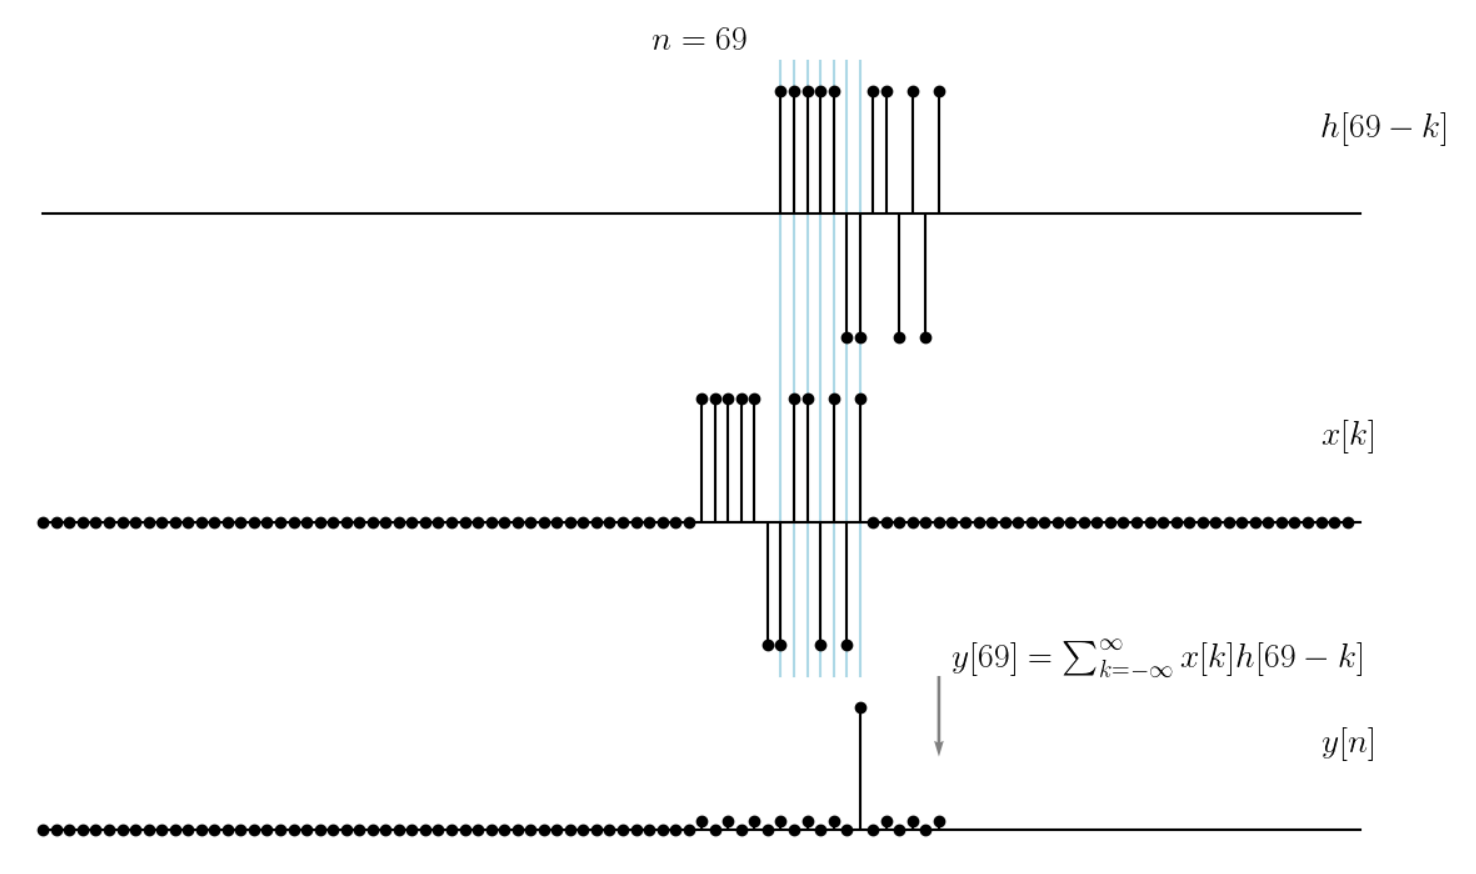
\includegraphics[width=\textwidth]{ch10/figures/ex_animation.png}
\caption{An example of the convolution operation for the 13-bit Barker code and the corresponding matched filter used often in radar and sonar applications to increase the effective power of the transmit pulse. The convolution of the matched filter $x^*[-n]$ and the transmit code $x[n]$ should be as close to a unit impulse $P\delta[n]$ as possible for a good radar transmit code. Here $P$ is a constant indicating how much power is contained within the pulse. This and other example animations of the convolution operation can be found under the \texttt{code/017\symbol{95}fir\symbol{95}animation} directory.}
\label{fig:fir_animation_example}
\end{figure}




\section{Applications of convolution}

This chapter only scratches the practical and theoretical uses of
convolution and linear time-invariant systems. I'll use two examples
to illustrate the application of a one-dimensional convolution
equation. Be aware that these are by no means the only types of
situations where you will encounter a convolution. Chances are quite
high that a signal processing system you can think of is an LTI
system, or can be approximated as one. Convolution can be found
everywhere!

\subsection{Example: Radar and sonar equation}

\begin{marginfigure}
\begin{center}
\includegraphics[width=\textwidth]{Applications/figures/svalbard.jpg}
\end{center}
\caption{EISCAT Svalbard Radar. The radar echo from the D-region of the ionosphere can be modeled using the equation shown in Equation \ref{eq:convolution_radar}. Photo: Craig Heinselman}
\label{fig:eiscat_svalbard}
\end{marginfigure}
The convolution equation is often used to model radar and sonar
measurements. In this case, the impulse response signal $h[n]$
represents the signal that is scattered as a function of distance. The
signal $x[n]$ represents what a radar or sonar transmits. The signal
received by a radar or sonar receiver $m[n]$ is then modeled as:
\begin{align}
m[n] &=  h[n]*x[n]\\
     &= \sum_{r=0}^{M} h[r] x[n-r]. \label{eq:convolution_radar}\,\,.
\end{align}
In this case, the index $r \in \mathbb{N}$ represents round-trip
propagation time between the transmitter and the receiver. The larger
the distance between the transmitter and the receiver, the larger the
delay. Assuming that the sample rate is $f_s$ in units of hertz or
($\frac{1}{\mathrm{s}}$), and the group velocity of the transmitter
wave $v_g$ ($\frac{\mathrm{m}}{\mathrm{s}}$), the round-trip range is given by:
\begin{equation}
R = \frac{v_g r}{2 f_s}\,\,.
\end{equation}
In the case of radar, the group velocity for electromagnetic waves is
$v_g \approx 3 \cdot 10^8$ ($\frac{\mathrm{m}}{\mathrm{s}}$). For sonar, it is the speed of
acoustic waves within the medium. In the case of air, this is
$v_g \approx 343$ ($\frac{\mathrm{m}}{\mathrm{s}}$).

To see how the convolution equation is the radar equation, we can use
an illustration, as shown in Figure \ref{fig:range_time_diagram}.
\begin{figure}
\begin{center}
\includegraphics[width=\textwidth]{Applications/figures/rd.pdf}
\end{center}
\caption{A range-time diagram depicting the relationship between a transmitted signal and a scattered signal.}
\label{fig:range_time_diagram}
\end{figure}

If the probing signal is a unit impulse $x[n]=\delta[n]$ (a very short
radar pulse), then the measurement directly provides the scattering
amplitude as a function of range:
\begin{align}
m[n] = \sum_{r=0}^M h[r]\delta[n-r] = h[r]\,\,.
\end{align}
This type of radar is called a pulsed radar. In terms of radar
signal processing, this is the easiest case, as no signal processing
is needed! A radar measurement in this case is equivalent to measuring
the ``impulse response'' of the region that the radar is probing.

Here is a fascinating example of a blind child that has learned to
click his tongue (emitting a $\delta[n]$-like impulse sound) to probe the
acoustic scattering of his
surroundings \url{https://www.youtube.com/watch?v=fnH7AIwhpik}. While
this may seem like a superhuman feat, this is not unlike measuring the
distance between yourself and a mountain side by shouting ``echo''
very loudly and counting how long it takes for you to hear a strong
echo. I am sure that many of you have done this already.

\begin{marginfigure}
\begin{center}
\includegraphics[width=\textwidth]{Applications/figures/mountain_echo.pdf}
\end{center}
\caption{The acoustics of a space are determined by acoustic waves
scattered from various obstacles at various propagation delays. This
can be quite precisely modeled using a convolution, assuming that
nothing is moving.}
\end{marginfigure}

If the transmitted waveform $x[n]$ is more complicated than a unit
impulse, the measurements need to be filtered in some way to
reconstruct the scattered signal as a function of range $h[n]$. This
is achieved by designing a filter $\lambda[n]$, which has the
following property $\lambda[n]*x[n] \approx \delta[n]$. After applying
the filter $\lambda[n]$ to the measured signal, one obtains the echo
as a function of range:
\begin{align}
\lambda[n]*m[n] = \lambda[n]*h[n]*x[n] = (\lambda[n]*x[n])*h[n]\approx h[n]\,\,. 
\end{align}
Design of pairs of signals $x[n]$ and filters $\lambda[n]$ is a topic
of radar signal processing. An example of a good pairing of a radar
transmit signal and a receiver filter is shown in Figure
\ref{fig:fir_animation_example}. This is the so-called 13-bit Barker
code. If the time-flipped and scaled 13-bit Barker code is used as the
deconvolution filter $\lambda[n]=13^{-1}x[-n]$, then the result is close to a unit impulse $\lambda[n]*x[n] \approx \delta[n]$.

\input{Applications/reverb}
\input{ch10/exercises10}
 \ifSpExerciseSol
 \input{ch10/solutions10}
 \fi
\fi

\ifSpFResp
\chapter{Frequency Response}
\input{ch11/text11}
\input{ch11/exercises11}
 \ifSpExerciseSol
 \input{ch11/solutions11}
 \fi
\fi

\ifSpProgB
\chapter{Programming Assignment 2}

\begin{marginfigure}[5cm]
  \begin{center}
    \includegraphics[width=\textwidth]{Assignments/figures/bat.jpg}
  \end{center}
  \caption{Bats use chirp-like ultrasound signals to sense their surroundings. Image: David Dennis.}
  \label{fig:bat_image}
\end{marginfigure}

This programming assignment deals with deconvolution of transmit
signals for an \emph{acoustic sounder} or a \emph{sonar}. A sonar is
a device that measures the amplitude of sound waves that are scattered
from objects at different propagation distances between the acoustic
wave transmitter and receiver. These devices are used, e.g., in cars to
assist with parking, in ships to measure the water depth, and for
non-invasive medical examinations. Sonars are also closely related
with radars, as they share many of the same signal processing
concepts. The main difference is that radars use electromagnetic waves
instead of acoustic waves.

In order to implement a simple sonar, I have used a loudspeaker and a
microphone connected to a sound card to transmit and receive acoustic
signals. The sampling rate of the audio recording is $f_s=44.1\cdot
10^3$ hertz, which results in a sample-spacing of $T_s=2.2676\cdot
10^{-5}$ s. The loudspeaker and the microphone are spaced apart by
approximately 2 cm.
 
If we ignore measurement errors, the acoustic signal can be modeled using
a discrete-time convolution equation:
\begin{equation}
  m[n] = \sum_{r=0}^{R-1} h[r]x[n-r] = h[n] * x[n]
  \label{eq:sonar_eq_pa}
\end{equation}
In this equation $m[n]$ is the signal measured with a microphone,
$x[n]$ is the signal transmitted by the loudspeaker, and $h[n]$ is
the amplitude of the scattered signal as a function of range. The
signal $h[n]$ is also the impulse response of the space that the sonar
is measuring. The convolution equation can be motivated with a
range-time diagram that models the propagation of acoustic signals as
a function of range and time. Such a diagram is shown in Figure
\ref{fig:range_time_diagram_ex}.

\begin{figure}
\begin{center}
\includegraphics[width=\textwidth]{Applications/figures/rd.pdf}
\end{center}
\caption{A range-time diagram depicting the relationship between a transmitted signal and a scattered signal.}
\label{fig:range_time_diagram_ex}
\end{figure}

Modern sonars often use long waveforms in order to compress more
energy into the transmitted pulse without increasing the amount of
peak power. Longer waveforms also make it easier to separate multiple
different transmitters from one another, reducing interference. 

One of the main objectives of a sonar measurement is to recover the impulse
response $h[n]$ from measurements $m[n]$. This is trivial when the
transmit pulse is a unit impulse $x[n]=A\delta[n]$. With longer
transmit signals, we need to deconvolve the transmitted signal. This
is typically achieved by convolving the received signal $m[n]$ with a 
deconvolution filter $\lambda[n]$:
\begin{equation}
  \lambda[n]*m[n] = \lambda[n] * x[n] * h[n].
\end{equation}
The deconvolution filter needs to have the following property:
\begin{equation}
  \lambda[n]*x[n] \approx A\delta[n],
\end{equation}
where $A$ is a constant. In the case of chirp-like signals, an often used 
deconvolution filter is the time reversed chirp signal:
\begin{equation}
  \lambda[n] = x[-n].
\end{equation}

For this assignment, I have used an amplitude tapered chirp-like
waveform with a linearly increasing frequency of the following form:
\begin{equation}
  x[n] = \left\{
\begin{array}{ccc}
  \sin^{0.5}\left(\frac{\pi n}{N}\right) \sin(2\pi \beta T_s^2 n^2) & \mathrm{when} & 0 \le n < N\\
  0 & \mathrm{otherwise} & 
  \end{array}\right.
\end{equation}
Here $N$ is the integer length of the chirp pulse in samples and
$\beta = \frac{1}{2 N T_s}f_{\mathrm{max}}$ is the chirp-rate, which
determines how fast the instantaneous frequency of the signal
increases as a function of time, with $f_{\mathrm{max}}$ the maximum
frequency used of the chirp (in hertz) at the end of the transmit
pulse. Figure \ref{fig:tx_pulse_chirp} shows this waveform with
$N=10000$ and $\beta = 33075 \text{s}^{-2}$.

\begin{marginfigure}
  \begin{center}
    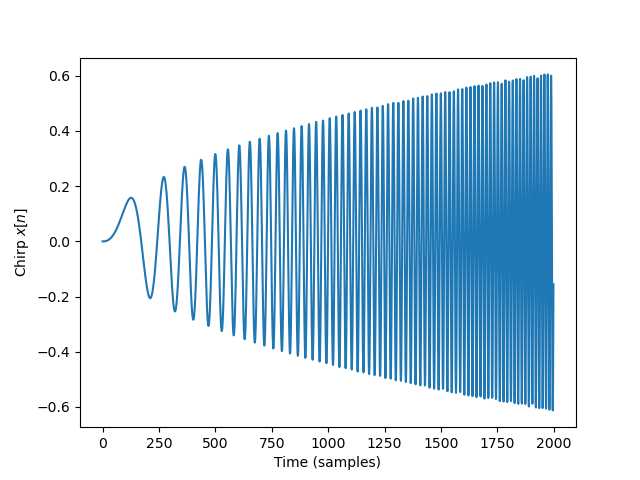
\includegraphics[width=\textwidth]{Assignments/figures/chirp_tx.png}
  \end{center}
  \caption{The first 2000 samples of the chirp transmit pulse signal
    $x[n]$.}
  \label{fig:tx_pulse_chirp}
\end{marginfigure}

You will need to download two data files for this task:
\begin{itemize}
  \item \url{https://github.com/jvierine/signal_processing_course/blob/main/code/027_sonar/chirp_2024.bin}
  \item \url{https://github.com/jvierine/signal_processing_course/blob/main/code/027_sonar/chirp_rec_2024.bin}
\end{itemize}
The first one contains the transmitted chirp waveform $x[n]$ and the
second one contains a microphone recording during a sonar experiment
$m[n]$.

You can read these signals into a
computer as follows:
\begin{lstlisting}[language=Python, numbers=none]
import matplotlib.pyplot as plt
import numpy as np

# Read chirp waveform.
chirp = np.fromfile("chirp_2024.bin", dtype=np.float32)
# Read microphone recording.
m = np.fromfile("chirp_rec_2024.bin", dtype=n.float32)

plt.plot(chirp)
plt.xlabel("Time (samples)")
plt.ylabel("Transmitted signal $x[n]$")
plt.show()

# Plot the first three interpulse periods.
plt.plot(m[:30000])
plt.xlabel("Time (samples)")
plt.ylabel("Received signal $m[n]$")
plt.show()
\end{lstlisting}
These acoustic signal in \verb|chirp_2024.bin| is transmitted every
$M=10000$ samples. This means that the sonar is repeating a
measurement of $h[n]$ every $10000$ samples and the transmitted signal
actually looks like this:
\begin{equation}
  \epsilon[n] = \sum_{k=0}^{N_p-1} x[n - Mk]
\end{equation}
In this task, you should treat each segment of 10000 samples as an
independent sonar measurement, which will allow you to study how the
impulse response $h[n]$ evolves over time. The first 30000 samples of the sonar echo are shown in Figure \ref{fig:rx_chirp}.
\begin{marginfigure}
  \begin{center}
    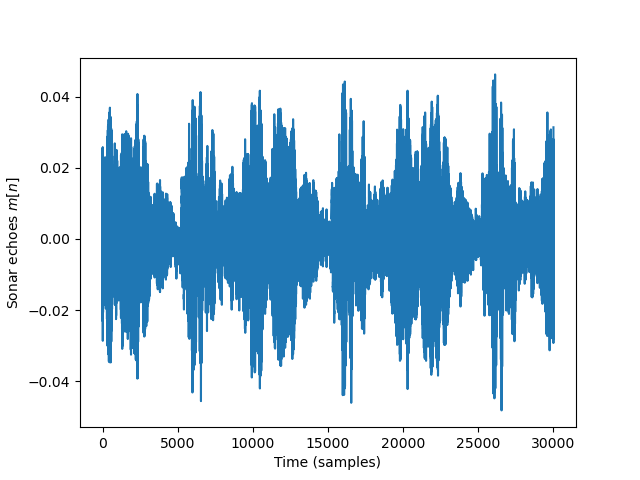
\includegraphics[width=\textwidth]{Assignments/figures/chirp_rec_2024.png}
  \end{center}
  \caption{The first 30000 samples of sonar echoes $m[n]$.}
  \label{fig:rx_chirp}
\end{marginfigure}

For this assignment, you are to perform the following tasks. Write a
short report describing what you did and what results you got. The
report is otherwise free form, as long as it is in PDF format. Include
your code and plots in the report. Please ensure that the report is
\textbf{less than three pages long}. Submit your solution to Canvas by
9.10. 12:00 if you want feedback. Keep a copy for submission at the
end of the course.

You will find a lot of help for this task in the lecture notes that
discusses LTI systems, convolution and frequency response. You may
help each other on Perusall. It is fine to give hints, but please try
not to give away the \emph{exact solution}.

\begin{enumerate}[a)]
  
\item What is the physical meaning of the signals $x[n]$ and $h[n]$ in
  Equation \ref{eq:sonar_eq_pa}?
  
\item What is the physical meaning of $r$ in Equation
  \ref{eq:sonar_eq_pa}?
  
\item How many meters of distance does an acoustic pulse travel during
  10000 samples? Assume sound speed in a typical lecture room
  at UiT (343 m/s).
  
\item How long is the transmitted sonar signal in seconds? The signal
  is in the file \verb|chirp_2024.bin|.

\item How long is the measurement in seconds? You can figure this out
  by looking at the length of the signal \verb|chirp_rec_2024.bin| and
  using the known sample-rate.
    
\item Why does the deconvolution filter $\lambda[n]$ need to have the
  property: $\lambda[n]*x[n] \approx A\delta[n]$, where $A$ is a constant?
   
\item Evaluate the autocorrelation function of the transmitted signal
  $c[n]=x[n]*x[-n]$. Use the signal that you read from
  \verb|chirp_2024.bin|. You can time-reverse a signal in Python using
  \verb|deconvolution_filter = x[::-1]|. Make a plot of $c[n]$ zooming
  into the portion of the signal that has significantly non-zero
  values. What are the implications of any deviations from a unit
  impulse for $c[n]$? Note that the function
  \verb|numpy.convolve(a,b,mode="same")| implements a convolution
  between signals $a[n]$ and $b[n]$.

%\item How close is $c[n]$ in your opinion to a scaled unit
 % impulse $A\delta[n]$? How will deviations from the unit impulse
 % affect deconvolution quality when using $\lambda[n]=x[-n]$ as a
  %deconvolution filter?
  
\item Make a plot of the scattered power as a function of time and
  range. Use one pulse for each column of the array that you are
  plotting.  You should get something similar to the plot in Figure
  \ref{fig:ex_rti_plot}. Use decibel scale for power. Use time in
  seconds on the x-axis and total propagation distance in meters on
  the y-axis. Total propagation distance means the total travelled
  distance between the loudspeaker and the microphone. You can use,
  e.g., the \verb|pcolormesh| command from Python's Matplotlib to
  make this plot. You will also find the NumPy function
  \verb|numpy.convolve(a,b,mode="same")| useful in this step.

\item Identify the strongest scatterer that is first moving away from
  the sonar, and then moving back towards the sonar. What is the
  furthest distance that the scatterer goes to before starting to move
  back towards the sonar in meters?
  
  \begin{figure}
  \begin{center}
    \includegraphics[width=\textwidth]{Assignments/figures/sonar_rti.png}
  \end{center}
  \caption{An example range-time intensity plot showing how much power
    in decibel scale is scattered back from the surroundings of the
    sonar system. The distance between the microphone and the
    loudspeaker is about 30 cm, which can be seen as a constant
    horizontal line at the propagation distance. The plot also shows
    an acoustic scatterer that is first moving away and then moving
    back towards the transmitter. Note that this is not the same plot
    that you will obtain with your data!}
  \label{fig:ex_rti_plot}
\end{figure}

\end{enumerate}

\fi

\ifSpDTFT
\chapter{Discrete-time Fourier Transform (DTFT)}
The equation for frequency response of a discrete-time linear
time-invariant system (Equation \ref{eq:dt_fr}) is also known as the
\emph{\index{Discrete-Time Fourier Transform}{Discrete-Time Fourier Transform}} (DTFT).
We can obtain a DTFT for an arbitrary discrete-time signal $x[n]$ as
follows\sidenote{Hat on top of $\hat{x}$ to signify that it is a
    frequency domain representation of signal $x[n]$, and a hat on top of
    $\hat{\omega}$ to signify that the frequency has units of radians per
    sample.}:
\begin{equation}
    \boxed{
        \hat{x}(\hat{\omega}) = \sum_{n=-\infty}^{\infty} x[n] e^{-i\hat{\omega} n}\,\,.
    }
    \label{eq:dtft_eq}
\end{equation}
Here $\hat{x}(\hat{\omega})$ is the DTFT of a discrete-time signal
$x[n]$. We'll use the following notation for denoting DTFT pairs:
\begin{equation}
    \boxed{
        x[n] \xleftrightarrow{\mathcal{F}} \hat{x}(\hat{\omega})
    }
\end{equation}
like we did in the Fourier transform chapter. The left-hand side
denotes the time domain representation, and the right-hand side
denotes the frequency domain representation.

Let's show that Equation \ref{eq:dtft_eq} is a special case of the
continuous-time Fourier transform for discretized signals. Remember
that the formula for discretizing a continuous-time signal is:
\begin{equation}
    x[n] = x(nT_s)\,\,.%\int_{-\infty}^{\infty} \delta(t-n T_s) x(t) dt.
\end{equation}
Here $T_s$ is the sample spacing, which is related to sample-rate
$f_s=1/T_s$. The continuous-time representation of the discretized
signal is defined as:
\begin{equation}
    x_d(t) = \sum_{n=-\infty}^{\infty} x[n] \delta(t-n T_s) \,\,.
\end{equation}
You might recall this from the derivation of the Whittaker-Shannon
sampling theorem. Figure \ref{fig:dirac_disc} depicts a
continuous-time signal and the continuous-time representation of the
discretized signal $x_d(t)$, which is a sequence of unit impulses
multiplied by the value of each discrete-time signal sample $x[n]$ at
the position in time, where it was sampled.
\begin{marginfigure}[-3cm]
    \begin{center}
        \begin{tikzpicture}
            \begin{axis}[domain=-2*3.1415:2*3.1415,
                    width=7cm,height=5cm,ymin=-2.5,xmin=0,ymax=2.5,xmax=6,
                    ytick={-1,1},
                    yticklabels={,,},
                    xticklabels={,,},
                    ylabel={$x(t),{\color{blue}x_d(t)}$},
                    xlabel=$t$, axis lines = center]
                \addplot+[dirac,samples=15] {-0.5+sin(deg(x))+0.5*sin(2*deg(0.5*x)-0.0)+0.7*sin(3*deg(x)-0.6)+0.3*sin(4*deg(x)+1.6)};
                \addplot[samples=200]{-0.5+sin(deg(x))+0.5*sin(2*deg(0.5*x)-0.0)+0.7*sin(3*deg(x)-0.6)+0.3*sin(4*deg(x)+1.6)};
                \node at (axis cs:0.9+0.45,1.1) [above, font={\footnotesize}]{$T_s$};
                \addplot [dimen,black]plot coordinates {(0.9,1.1) (2.0*0.9,1.1)};

                %\addplot +[dirac] coordinates {(1,1)};
            \end{axis}
        \end{tikzpicture}
    \end{center}
    \caption{A continuous-time signal $x(t)$ and a continuous-time representation of 
    a discretized signal $x_d(t)$. Sample spacing $T_s$ is related to sample rate as follows: $T_s = 1/f_s$.}
    \label{fig:dirac_disc}
\end{marginfigure}

The Fourier transform of $x_d(t)$ is
\begin{equation}
    \hat{x}_d(\omega) = \int_{-\infty}^{\infty} x_d(t) e^{-i\omega t}dt\,\,.
    \label{ctft}
\end{equation}
This can be simplified as follows:
\begin{align}
    \hat{x}_d(\omega) & =\int_{-\infty}^{\infty} \left(\sum_{n=-\infty}^{\infty} \delta(t- nT_s) x[n]\right) e^{-i\omega t}dt \\
                      & =\sum_{n=-\infty}^{\infty} \int_{-\infty}^{\infty} \delta(t-nT_s) x[n] e^{-i\omega t}dt               \\
                      & = \sum_{n=-\infty}^{\infty} x[n] e^{- i \omega n T_s}\label{eq:dtftd1}\,\,.
\end{align}
If we substitute $\hat{\omega}=\omega T_s$, we get\sidenote{This also implies that $\hat{x}(\hat{\omega})
        = \hat{x}_d(\omega/T_s)$}:
\begin{equation}
    \hat{x}(\hat{\omega}) = \sum_{n=-\infty}^{\infty} x[n] e^{- i \hat{\omega} n}\qed\,\,.
\end{equation}
This shows that the discrete-time
Fourier transform is a special case of the continuous-time Fourier
transform for discretized signals, and that $\hat{x}(\hat{\omega})$ is
the frequency domain representation of the discrete-time signal
$x[n]$.

The fact that the discrete-time Fourier transform is a Fourier
transform means that all the properties of a Fourier transform also
apply to the discrete-time Fourier transform. However, there are some
special properties of the discrete-time Fourier transform, which we
will go through.

\section{Periodicity}

The DTFT $\hat{x}(\hat{\omega})$ is a $2\pi$-periodic function:
\begin{equation}
    \boxed{
        \hat{x}(\hat{\omega})=\hat{x}(\hat{\omega}+2\pi k)
    }
\end{equation}
with $k \in \mathbb{Z}$. This is relatively easy to show:
\begin{align}
    \hat{x}(\hat{\omega}+2\pi k) & = \sum_{n=-\infty}^{\infty} x[n]e^{-i(\hat{\omega}+2\pi k)n}                         \\
                                 & = \sum_{n=-\infty}^{\infty} x[n]e^{-i\hat{\omega}n} \underbrace{e^{-i 2\pi nk}}_{=1} \\
                                 & = \hat{x}(\hat{\omega})\qed\,\,.
\end{align}

\begin{marginfigure}[-6cm]
    \begin{center}
        \begin{tikzpicture}
            \begin{axis}[width=7cm,
                domain=(-3*3.14):(3*3.14),
                samples=400,
                xmin=-12,
                xmax=12,
                ymin=-0.5,
                ymax=1.2,
                legend style={draw=none,at={(.99,.1)},anchor=south east},
                xlabel={$\hat{\omega}$},
                ylabel={$|D_{21}(\hat{\omega})|$},
                axis x line=center,
                axis y line=middle,
                ytick={0,1},
                xtick={-6.28,-3.14,0,3.14,6.28},
                xticklabels={$-2\pi$,$-\pi$,0,$\pi$,$2\pi$}
                ]
                \addplot[blue] {abs(sin(deg(x*(10+0.50000001)))/(21*sin(1e-6+deg(x/2.0))))};
            \end{axis}
        \end{tikzpicture}
        \begin{tikzpicture}
            \begin{axis}[width=7cm,
                domain=(-3*3.14):(3*3.14),
                samples=400,
                xmin=-12,
                xmax=12,
                ymin=-0.5,
                ymax=1.2,
                legend style={draw=none,at={(.99,.1)},anchor=south east},
                xlabel={$f$},
                ylabel={$|D_{21}(f)|$},
                axis x line=center,
                axis y line=middle,
                yticklabels={,,},
                xtick={-6.28,-3.14,0,3.14,6.28},
                xticklabels={$-f_s$,$-f_s/2$,0,$f_s/2$,$f_s$}
                ]
                \addplot[blue] {abs(sin(deg(x*(10+0.50000001)))/(21*sin(1e-6+deg(x/2.0))))};
            \end{axis}
        \end{tikzpicture}
    \end{center}
    \caption{A discrete-time Fourier transform is $2\pi$-periodic in frequency domain. The top figure shows the magnitude response of the running average filter $|D_{21}(\hat{\omega})|$ with frequency in units of radians per sample on the x-axis. Bottom: The same as the above, but with x-axis with frequency in units of cycles per second. The sampling-rate $f=\pm f_s/2$ corresponds to $\hat{\omega}=\pm \pi$.}
    \label{fig:dir_kernelp}
\end{marginfigure}

The periodicity property is the same one that we encountered when
investigating aliasing of complex sinusoidal discrete-time signals,
which are essentially frequency components of a discrete-time
signal. Figure \ref{fig:dir_kernelp} shows one example of a
discrete-time Fourier transform, the Dirichlet kernel, that we
encountered when investigating the frequency response of a running average filter.

\section{Inverse transform}
The reverse operation is the inverse discrete-time Fourier transform,
which is defined as:
\begin{equation}
    \boxed{
    x[n] = \frac{1}{2\pi}\int_{-\pi}^{\pi} \hat{x}(\hat{\omega})e^{i\hat{\omega}n} d\hat{\omega}\,\,.
    \label{eq:idtft_def}
    }
\end{equation}
This allows transforming a discrete-time frequency domain
representation $\hat{x}(\hat{\omega})$ to a discrete-time signal $x[n]$.

It is quite easy to show that this inverse formula recovers $x[n]$ for
a DTFT $\hat{x}(\hat{\omega})$ that is defined as\sidenote{The inverse
    transform is nearly the same as the Fourier series analysis equation
    with $x[n]$ being the Fourier series coefficients and $\hat{x}(\hat{\omega})$ being a $2\pi$-periodic function.}:
\begin{equation}
    \hat{x}(\hat{\omega}) = \sum_{n=-\infty}^{\infty} x[n] e^{-i\hat{\omega} n}\,\,,
\end{equation}
we can recover $x[n]$ using the inverse transform formula:
\begin{align}
    \mathcal{F}^{-1}\left\{\hat{x}(\hat{\omega})\right\} & =\frac{1}{2\pi}\int_{-\pi}^{\pi} \hat{x}(\hat{\omega})e^{i\hat{\omega}n} d\hat{\omega}                                            \\
                                                         & =\frac{1}{2\pi}\int_{-\pi}^{\pi} \left[\sum_{m=-\infty}^{\infty} x[m]e^{-i\hat{\omega}m} \right] e^{i\hat{\omega}n} d\hat{\omega} \\
                                                         & =\frac{1}{2\pi}\sum_{m=-\infty}^{\infty} \int_{-\pi}^{\pi} x[m]e^{i\hat{\omega}(n-m)} d\hat{\omega}                               \\
                                                         & =\frac{1}{2\pi}\sum_{m=-\infty}^{\infty} 2\pi \delta[m-n] x[m]                                                                    \\
                                                         & =x[n]\qed
\end{align}
Here $\mathcal{F}^{-1}\{\cdot\}$ refers to the inverse DTFT.

We now have an inverse and forward discrete-time Fourier transform pair:
\begin{equation}
    \boxed{
    x[n] = \frac{1}{2\pi}\int_{-\pi}^{\pi} \hat{x}(\hat{\omega})e^{i\hat{\omega}n} d\hat{\omega} \xleftrightarrow{\mathcal{F}}
    \hat{x}(\hat{\omega}) = \sum_{n=-\infty}^{\infty} x[n] e^{-i\hat{\omega}n}\,\,.
    }
\end{equation}
We'll now list several discrete-time Fourier transform pairs. Note
that many of these have in fact already been discussed in the chapter
on the continuous-time Fourier transform.

\if 0
    \section{Frequency response for a real-valued impulse response}

    The frequency response of a real-valued impulse-response
    $h[n]\in \mathbb{R}$ is conjugate symmetric
    \begin{equation}
        \boxed{
            \He^* = \mathcal{H}(-\hat{\omega})\,\,.
        }
        \label{eq:conj_symmetry_lti}
    \end{equation}
    We can quite easily prove this:
    \begin{align}
        \He^* & = \left(\sum_k h[k] e^{-i\hat{\omega}k}\right)^* \\
              & = \sum_k h[k]^* e^{i\hat{\omega}k}               \\
              & = \sum_k h[k] e^{i\hat{\omega}k}                 \\
              & = \mathcal{H}(-\hat{\omega})\,\,.
    \end{align}
    This follows from two facts: $(e^{i\phi})^* = e^{-i\phi}$ and $h[n]^*
        = h[n]$.

    We have already shown in the Fourier transform chapter that conjugate
    symmetry is a more general property of the Fourier transform of real
    valued signals. This is just a special case of this more general
    property that is applied to discrete-time signals.

    A corollary of Equation \ref{eq:conj_symmetry_lti} of this is that the
    magnitude response of an LTI system with a real-valued impulse
    response is always symmetric around zero:
    \begin{equation}
        \boxed{
            |\He| = |\mathcal{H}(-\hat{\omega})|\,\,.
        }
    \end{equation}

    \subsection{Example: real-valued cosine and real-valued impulse response}

    Let's investigate the output of an LTI system with a real-valued
    impulse response $h[n]\in\mathbb{R}$ when the input signal is a real-valued cosine signal
    \begin{equation}
        x[n] = A\cos(\hat{\omega} n + \phi)\,\,.
    \end{equation}
    Using Euler's formula, we can express the input signal as a sum of a
    positive and negative frequency complex sinusoidal signal:
    \begin{equation}
        x[n] = A \cos(\hat{\omega} n + \phi) = \frac{A}{2}e^{i\phi}e^{i\hat{\omega} n} + \frac{A}{2}e^{-i\phi}e^{-i\hat{\omega} n}\,\,.
    \end{equation}
    In this case, the output of the LTI system is:
    \begin{align}
        y[n] & = h[n]*x[n]                                                                                                                                                                           \\
             & = \sum_{k} h[k]x[n-k]                                                                                                                                                                 \\
             & = \sum_{k} h[k] \left( \frac{A}{2}e^{i\phi}e^{i\hat{\omega} (n-k)} + \frac{A}{2}e^{-i\phi}e^{-i\hat{\omega} (n-k)} \right)                                                            \\
             & = \left(\sum_{k} h[k] e^{-i\hat{\omega} k}\right) \frac{A}{2}e^{i\phi}e^{i\hat{\omega} n} + \left(\sum_{k} h[k] e^{i\hat{\omega} k}\right) \frac{A}{2}e^{-i\phi} e^{-i\hat{\omega} n} \\
             & = \mathcal{H}(\hat{\omega}) \frac{A}{2}e^{i\phi}e^{i\hat{\omega} n} + \mathcal{H}(-\hat{\omega}) \frac{A}{2}e^{-i\phi}e^{-i\hat{\omega} n}\,\,.
    \end{align}
    In this case, the impulse response is real-valued $h[n]\in \mathbb{R}$, and thus:
    \begin{equation}
        \mathcal{H}(-\hat{\omega}) = \mathcal{H}(\hat{\omega})^*\,\,.
    \end{equation}
    This means that we can write the output signal as a sum:
    \begin{align}
        y[n] & = \He \frac{A}{2}e^{i\phi}e^{i\hat{\omega} n} +  \He^*\frac{A}{2}e^{-i\phi} e^{-i\hat{\omega} n}\,\,.
    \end{align}
    Which means that the spectral components are conjugate symmetric. The output of the real-valued sinusoidal signal is then:
    \begin{align}
        y[n] & = |\He|\frac{A}{2} e^{i(\phi + \angle \He)}e^{i\hat{\omega} n} + |\He|\frac{A}{2}e^{-i(\phi + \angle \He)} e^{-i\hat{\omega} n} \\
             & = |\He| A \cos(\hat{\omega} n + \phi + \angle \He)\,\,.
    \end{align}
    The output signal is a cosine signal with the same frequency as the
    input signals. The amplitude is scaled with the magnitude response
    $|\He|$ and the phase is shifted by $\angle \He$.

\fi




\usetikzlibrary{arrows.meta, positioning, quotes}
\begin{marginfigure}
    \begin{center}
        \begin{tikzpicture}[
            node distance=5mm and 20mm,
            box/.style = {draw, minimum height=12mm, align=center},
            sy+/.style = {yshift= 2mm},
            sy-/.style = {yshift=-2mm},
            every edge quotes/.style = {align=center}
            ]
            \node (n1) [box]             {$h[n]$\\Time domain};
            \node (n2) [box,right=of n1] {$\He$\\Frequency domain};
            %
            \draw[thick,-Triangle]
            ([sy+] n1.east) to [above] ([sy+] n2.west);
            \draw[thick,-Triangle, dashed]
            ([sy-] n2.west) -- ([sy-] n1.east);
        \end{tikzpicture}
    \end{center}
    \caption{The frequency response $\He$ of an LTI system is the Fourier transform of the impulse response $h[n]$.}
\end{marginfigure}

\section{Frequency response}

The frequency response of a discrete-time LTI system (shown earlier in Equation \ref{eq:dt_fr})
\begin{equation}
    \He = \sum_{k=-\infty}^{\infty} h[k] e^{-i\hat{\omega} k}
\end{equation}
is a discrete-time Fourier transform of the impulse response
$h[n]$. This means that all the properties of a discrete-time Fourier
transform will apply also to a frequency response. Using our short
hand notation, we can define this as a DTFT pair:
\begin{equation}
    \boxed{
        h[n] \xleftrightarrow{\mathcal{F}} \He\,\,.
    }
\end{equation}
The inverse DTFT formula will come in handy when, e.g., defining LTI
systems based on their frequency response characteristics, and then
obtaining the impulse response using the inverse transform. This leads
to, e.g., ideal filters, ideal frequency selective filters, and
arbitrary time shift filters. These are LTI systems that would be
difficult or impossible to derive in time domain.

\section{Time-shifted unit impulse}

DTFT for unit impulse is:
\begin{equation}
    \boxed{
        x[n] = \delta[n-n_0] \xleftrightarrow{\mathcal{F}} \hat{x}(\hat{\omega}) = e^{-i\hat{\omega}n_0}\,\,.
    }
\end{equation}
The proof is trivial.

\section{Frequency shift $e^{i\hat{\omega}_0n}x[n]$}

A shift in frequency domain corresponds to multiplication
by a complex exponential signal in time domain.  If
\begin{equation}
    x[n] \xleftrightarrow{\mathcal{F}} \hat{x}(\hat{\omega})\,\,,
\end{equation}
then
\begin{equation}
    \boxed{
    e^{i\hat{\omega}_0 n}x[n] \xleftrightarrow{\mathcal{F}} \hat{x}(\hat{\omega}-\hat{\omega}_0)\,\,.
    }
\end{equation}
The proof is as follows. If we multiply the signal $x[n]$ with a
complex exponential signal with frequency $\hat{\omega}_0$, we obtain a
new signal $y[n]$:
\begin{equation}
    y[n] = e^{i\hat{\omega}_0 n}x[n]\,\,.
\end{equation}
If we DTFT this, we obtain:
\begin{align}
    \hat{y}(\hat{\omega}) & =\sum_{k=-\infty}^{\infty} e^{i\hat{\omega}_0 k}x[k]e^{-i\hat{\omega}k}                                              \\
                          & =\sum_{k=-\infty}^{\infty} x[k] e^{-i(\hat{\omega}-\hat{\omega}_0)k} = \hat{x}(\hat{\omega}-\hat{\omega}_0)\qed\,\,.
\end{align}
Multiplying a time domain signal by a complex sinusoid with frequency
$\hat{\omega}_0$ results in a frequency shift of the signal in
frequency domain.

This property is useful for creating a filter with a specific center
frequency. This property can also be used to shift the center
frequency of a signal in frequency domain, e.g., in digital up or
down conversion systems that are found in digital radios.

\section{Convolution theorem}
An often used theorem of signal processing is the convolution theorem. It
states that convolution in time domain is multiplication in frequency
domain. This also applies to discrete-time Fourier transforms.
\begin{equation}
    \boxed{
    a[n] = b[n]*c[n] \xleftrightarrow{\mathcal{F}} \hat{a}(\hat{\omega}) = \hat{b}(\hat{\omega})\hat{c}(\hat{\omega})\,\,.
    }
\end{equation}
The proof is identical to the proof shown in the chapter on Fourier transforms.

\begin{marginfigure}

    \begin{center}
        \begin{tikzpicture}[node distance=3cm,auto,>=latex']

            \node [int] (a) {LTI $(h_1[n])$};
            \node [above of=a, node distance=1cm] (in) {$x[n]$};
            \node [int, below of=a, node distance=1cm] (b) {LTI $(h_2[n])$};
            \node [below of=b, node distance=1cm] (out) {$y[n]$};
            \path[->] (a) -> (b);
            \draw[->] (a) -> (b);
            \path[->] (in) -> (a);
            \draw[->] (in) -> (a);
            \path[->] (b) -> (out);
            \draw[->] (b) -> (out);

            \node [int, right of=a,node distance=2cm] (a3) {LTI $(h_3[n])$};
            \node [above of=a3, node distance=1cm] (in3) {$x[n]$};
            \node [below of=a3, node distance=1cm] (out3) {$y[n]$};
            \path[->] (in3) -> (a3);
            \draw[->] (in3) -> (a3);
            \path[->] (a3) -> (out3);
            \draw[->] (a3) -> (out3);

        \end{tikzpicture}
    \end{center}
    \caption{A consequence of the associative property of convolution is
    that two LTI systems characterized with $h_1[n]$ and $h_2[n]$ can be
    combined as a single LTI system with impulse response
    $h_3[n]=h_1[n]*h_2[n]$. The convolution theorem allows us to
    investigate the combined frequency response of the system using the following formula:
    $\mathcal{H}_3(\hat{\omega})=\mathcal{H}_1(\hat{\omega})\mathcal{H}_2(\hat{\omega})$.}
    \label{fig:cascade_lti}
\end{marginfigure}


\subsection{Example: cascaded filters}

A consequence of the convolution theorem is that we can analyze the
combined effect of a cascaded system, simply by multiplying together
the frequency responses.

Let's assume that a signal is first convolved with a filter that has
an impulse response $h_1[n]$ and then with a filter that has an
impulse response $h_2[n]$:
\begin{align}
    y[n] & = h_2[n]*(h_1[n]*x[n]) \\
         & = (h_1[n]*h_2[n])*x[n] \\
         & = h_3[n]*x[n]\,\,.
\end{align}
The combined frequency response $\mathcal{H}_3(\hat{\omega})$ of the
cascaded system is $\mathcal{H}_1(\hat{\omega})\mathcal{H}_2(\hat{\omega})$:
\begin{equation}
    \boxed{
    h_3[n]=h_1[n]*h_2[n] \xleftrightarrow{\mathcal{F}} \mathcal{H}_3(\hat{\omega}) = \mathcal{H}_1(\hat{\omega})\mathcal{H}_2(\hat{\omega})
    }
\end{equation}
where $\mathcal{H}_1(\hat{\omega})$ and $\mathcal{H}_2(\hat{\omega})$
are the frequency responses corresponding to impulse responses
$h_1[n]$ and $h_2[n]$.

\if 0
    \subsection*{Proof}
    Consider the convolution of two signals $a[n]$ and $b[n]$:
    \begin{align}
        Y(e^{i\hat{\omega}}) = a[n]*b[n] = \sum_k a[k] b[n-k]\,\,.
    \end{align}
    The discrete-time Fourier transform of these signals is:
    \begin{align}
        Y(e^{i\hat{\omega}}) & = \sum_n (a[n]*b[n]) e^{-i\hat{\omega}n}                          \\
                             & = \sum_n \left(\sum_k a[k]b[n-k]\right) e^{-i\hat{\omega}n}       \\
                             & = \sum_k a[k] \left(\sum_n b[n-k] e^{-i\hat{\omega}n}\right)\,\,.
    \end{align}
    If we now do a variable substitution: $n-k=\ell$, we obtain:
    \begin{align}
        Y(e^{i\hat{\omega}}) & = \sum_k a[k] \left(\sum_\ell b[\ell] e^{-i\hat{\omega}(\ell+k)}\right)                              \\
                             & = \left(\sum_k a[k] e^{-i\hat{\omega}k}\right) \left(\sum_\ell b[\ell] e^{-i\hat{\omega}\ell}\right) \\
                             & = A(e^{i\hat{\omega}})B(e^{i\hat{\omega}})\,\,.
    \end{align}
    This means that convolution is equivalent to multiplication in frequency domain.

    \subsection*{Alternate proof}

    A convolution is defined as:
    \begin{align}
        y[n] & = a[n] * b[n]             \\
             & = \sum_k a[k] b[n-k]\,\,.
    \end{align}
    Now we know that $a[n]$ and $b[n]$ have a discrete-time Fourier transform representation:
    \begin{align}
        A(e^{i\hat{\omega}}) & = \sum_k a[k] e^{-i\hat{\omega}k}      \\
        B(e^{i\hat{\omega}}) & = \sum_k b[k] e^{-i\hat{\omega}k}\,\,.
    \end{align}
    and inverse discrete-time Fourier transforms:
    \begin{align}
        a[n] & = \frac{1}{2\pi}\int_{-\pi}^{\pi}A(e^{i\hat{\omega}})e^{i\hat{\omega}n}d\hat{\omega}      \\
        b[n] & = \frac{1}{2\pi}\int_{-\pi}^{\pi}B(e^{i\hat{\omega}})e^{i\hat{\omega}n}d\hat{\omega}\,\,.
    \end{align}
    If we insert $b[n]$ as a function of $B(e^{i\hat{\omega}})$ into the convolution equation, we get
    \begin{align}
        y[n] & = \sum_k a[k]\frac{1}{2\pi}\int_{-\pi}^{\pi}B(e^{i\hat{\omega}})e^{i\hat{\omega}(n-k)}d\hat{\omega}                               \\
             & = \frac{1}{2\pi}\int_{-\pi}^{\pi}\left(\sum_k a[k] e^{-i\hat{\omega}k} \right)B(e^{i\hat{\omega}})e^{i\hat{\omega}n}d\hat{\omega} \\
             & = \frac{1}{2\pi}\int_{-\pi}^{\pi}A(e^{i\hat{\omega}})B(e^{i\hat{\omega}})e^{i\hat{\omega}n}d\hat{\omega}\,\,.
    \end{align}
    We can again see that convolution is multiplication in frequency domain.
\fi



\input{ch12/exercises12}
 \ifSpExerciseSol
 \input{ch12/solutions12}
 \fi
\fi

\ifSpFilters
\chapter{Ideal and Tapered Filters}
\input{ch13/text13}
\input{ch13/exercises13}
 \ifSpExerciseSol
 \input{ch13/solutions13}
 \fi
\fi

\ifSpUncertainty
\chapter{Time-frequency Uncertainty Principle}
\input{ch14/text14}
\input{ch14/exercises14}
 \ifSpExerciseSol
 \input{ch14/solutions14}
 \fi
\fi

\ifSpDFT
\chapter{Discrete Fourier Transform}
\input{ch15/text15}
\input{ch15/exercises15}
 \ifSpExerciseSol
 \input{ch15/solutions15}
 \fi
\fi

\ifSpSpectAn
\chapter{Spectral Analysis}
\input{ch16/text16}
\input{ch16/exercises16}
 \ifSpExerciseSol
 \input{ch16/solutions16}
 \fi
\fi

\ifSpFiltering
\chapter{Arbitrary Frequency Response Filters}
\input{ch17/text17.tex}
\input{ch17/exercises17}
 \ifSpExerciseSol
 \input{ch17/solutions17}
 \fi
\fi

\ifSpProgC
\chapter{Programming Assignment 3}

\begin{marginfigure}
  \begin{center}
    \includegraphics[width=\textwidth]{Assignments/figures/nsf_ligo.jpg}
  \end{center}
  \caption{Artist's depiction of gravitational waves created by a merger of two neutron stars. Credits: US National Science Foundation.}
\end{marginfigure}

In 2017, the Nobel Prize in physics was awarded to Rainer Weiss, Barry
Barish and Kip Thorne for the discovery of gravitational waves. Only
two years earlier, on September 14, 2015, 09:50:45 UTC, the two Laser
Interferometer Gravitational-Wave Observatory (LIGO) instruments
detected a gravitational wave for the first time in
history. Gravitational waves were predicted by Einstein’s general
theory of relativity but had never been detected in situ before.

The first gravitational wave event detected by LIGO is thought to be
created from a collision of two black holes, which sends out a
localized chirp-like pulse in the space-time. LIGO utilizes two
detectors, which are spaced 3000 km apart. These detectors measure
\emph{strain} ($\Delta L/L$) as a function of time. Here $\Delta L$ is
the variation in length and $L$ is the total length in which the
variation is measured. In other words, strain is the normalized
variation in length $L$ of the interferometer line due to
gravitational-wave. Figure \ref{fig:ligo_nobel_diag} provides a high
level overview of the measurement.

LIGO uses two geographically separated stations to measure gravitational
waves: Hanford (H$_1$), and Livingston (L$_1$). The gravitational wave
propagates at the speed of light $c\approx 3\cdot 10^8$
$\mathrm{m}/\mathrm{s}$. If the same signal is detected at two
different places with a time difference less than or equal to the
speed of light propagation time between the sensors, then this
provides more confidence that the event is in fact real, and not
caused by for example local seismic activity. A third sensor would
allow determining the direction of arrival based on time of arrival.

\begin{marginfigure}
  \begin{center}
    \includegraphics[width=\textwidth]{Assignments/figures/hanliv.jpg}
  \end{center}
  \caption{The Hanford and Livingston interferometers. Credits: LIGO.}
\end{marginfigure}

The LIGO data is severely corrupted with instrumental noise. This
noise is much larger in amplitude than the gravitational wave
signal. However, this noise is very narrowband in nature, and it can
be filtered out using relatively basic signal processing techniques
without affecting the relatively broad band gravitational signal very
much. Such filtering is routinely used by LIGO to improve the
sensitivity of the instrument.

Verification of scientific results is an important part of
science. UiT does not have the resources for building a giant
interferometer, and this course really isn't about solving Einstein's
field equations, so we won't be able to reproduce all the
results. However, we can verify the signal processing part. In this
programming assignment, your task is to develop signal processing
software to verify that you can detect the gravitational wave
signature in the LIGO measurements.


\section{Instructions}

We expect you to complete the listed signal processing tasks. The
submission form is a written report that answers the questions given
in each part of this assignment. The report should include the code
with comments that indicate what each part of the program
does. \textbf{The report should have at most five pages}. You can
return your report on Canvas by November 4th to receive feedback
before the final portfolio submission on November 11th. The final
portfolio submission including all three programming assignments will
be on Wiseflow on November 11th.



% In the first part, you have already completed sections 3-7. For this
% second part of the assignment, you need to complete sections
% 8-13. You may choose to continue your previous report, or to write a
% new report that just covers sections 8-13.

You only need to know about signal processing concepts taught in
FYS-2006. You do not need to know anything about gravitational waves
or the LIGO instrument in order to complete the assignment. The
lecture notes for the course contain several helpful signal processing
examples. Take a look at lecture notes on \emph{spectral analysis},
and \emph{arbitrary frequency response filters}.


\section{Instruction for reading the data}

To begin, download the data files and a simple program that
demonstrates reading these files from this location:
\url{code/029_ligo}. The data files are:
\begin{verbatim}
H-H1_LOSC_4_V2-1126259446-32.hdf5
L-L1_LOSC_4_V2-1126259446-32.hdf5
\end{verbatim}
These data files contain real measurements from LIGO starting at
2015-09-14T09:50:30 UTC.

After downloading the files, the next step is to read the strain
signal from the data files. In Python, this can be done using the h5py
module\sidenote{Make sure you have the h5py module installed on your
  computer!}.
\begin{verbatim}
import h5py
h = h5py.File("file.hdf5","r")
data = h["strain/Strain"][()]
\end{verbatim}
You will need to read two data vectors. One for the Livingston station
(L$_1$) and one for the Hanford station (H$_1$). We will use the symbol $x_H[n]$
of the Hanford signal and $x_L[n]$ for the Livingston signal.

\section{1. Data}
The sample rate of both of the signals is $f_s=4096$ Hz. The samples
in both signals are synchronized in time, i.e., sample $n$ in signal
$x_H[n]$ and $x_L[n]$ occur at the same time. Start by writing code to
read the Hanford and Livingston signals from the data file.
\begin{enumerate}[a)]
  \item How many samples are in each of the signals: $x_H[n]$ and $x_L[n]$?
  \item How many seconds long is each signal $x_H[n]$ and $x_L[n]$ in
    the dataset?
\end{enumerate}

\section{2. Plotting the data}

In order to see what the signals look like, you will need to plot the data.
\begin{enumerate}[a)]
  \item Plot the signals $x_H[n]$ and $x_L[n]$, with time in seconds on
        the horizontal axis and strain on the vertical axis. Assume that
        time at the beginning of the signal array starts at $0$ seconds. Label
        the axes of your plot. Use separate plots for $x_H[n]$ and $x_L[n]$
        signals. Hint: you can use the \verb|plt.plot(t,signal)| command found
        in Matplotlib. Use an array \verb|t| to denote the seconds of each sample of the array \verb|signal|.

\end{enumerate}

\section{3. Selecting a tapered window function}

You will need to apply a discrete Fourier transform to analyze the
spectral content of the signal. You will need to select a suitable
tapered window function in order to obtain a good rejection of out of
band signals. This will be crucial for detecting the real LIGO signal
later. In this task, we'll use a synthetic narrowband signal to
compare the performance of a discrete Fourier transform (DFT) based
spectral analysis using a tapered window to spectral analysis done
without a tapered window.

In order to calculate the magnitude spectrum of a signal $x[n]$ of length $N$, you need to evaluate a DFT on the signal:
\begin{equation}
  \hat{x}[k] = \sum_{n=0}^{N-1} x[n] e^{-i\frac{2\pi}{N}kn}.
  \label{one}
\end{equation}
and the windowed signal:
\begin{equation}
  \hat{x}_w[k] = \sum_{n=0}^{N-1} w[n]x[n] e^{-i\frac{2\pi}{N}kn}.
\end{equation}
Hint: Use the \verb|fft| function to evaluate the
DFT. This function is available in Python as \verb|numpy.fft.fft|.


\begin{enumerate}[a)]
  \item Find Python functions in scipy that implement the Hann and
    Hamming windows.  You can use tapering window functions available
    in the \verb|scipy.signal| module.

  \item In order to get an idea of how the window functions behave,
    apply it to a test signal consisting of two sinusoids. One with a
    weak amplitude and one with a strong amplitide.
        \begin{equation}
          x[n]=10^{-5}\cos(2\pi 31.5  n/f_s) + \cos(2*\pi*1234.56 n/f_s)
        \end{equation}
        Use a sample-rate of 4096 Hz. The frequencies of the sinusoids
        are 31.5 Hz and 1234.56 Hz, and the amplitudes $10^{-5}$ and 1
        as shown in the above equation.  Sample signal at sample
        indices $n\in[0,1,2,\cdots,4095]$. Make a plot of the signal
        $x[n]$ and the windowed signal $w[n]x[n]$. Use a window of the
        same length as your signal $N=4096$. Hint: You can use
        \verb|numpy.arange(N)| to create a sequence of integers
        between $0$ and $N-1$.

  \item The FFT algorithm will evaluate $\hat{x}[k]$ at integer values of $k$ between $0$ and $N-1$.
        What frequencies $f_k$ in hertz do frequencies $\hat{\omega}_k = 2\pi k/N$ in radians per sample
        correspond to on the principal spectrum ($-f_s/2 < f_k < f_s/2$)?

  \item Which values of $k$ correspond to a frequency $f_k$ that is nearest to $31.5$ and $-31.5$ hertz?

  \item Estimate the power spectrum of the windowed signal $w[n]x[n]$
    (with tapering) and the signal $x[n]$ (without tapering). Plot the
    power spectrum in decibel scale (power) for both.  Use frequency
    in Hz on the horizontal axis and magnitude squared $10
    \log_{10}(|\hat{x}[k]|^2)$ (decibels) on the vertical axis.  Plot
    both the positive and negative frequencies. Hint: You can use
    \verb|numpy.fft.fftfreq| and \verb|numpy.fft.fftshift| to
    determine what frequency (in hertz) each FFT bin $k$ corresponds
    to, and to order the frequencies in ascending order.

      \item Mark the locations of 31.5 and 1234.56 Hz in the plot

      \item Does the rectangular window (no tapering) allow you to detect the 31.5 Hz spectral line?
        
      \item Compare the Hann and Hamming windows. Which one allows you
        to detect the weak signal better? Use the tapering window that
        works best in the next section.
\end{enumerate}

\section{4. Estimating the spectrum of the LIGO signal}

\begin{enumerate}[a)]
  \item Calculate the power spectrum of the LIGO signals
        $|\hat{x}_L[k]|^2$ and $|\hat{x}_H[k]|^2$. Here $\hat{x}_L[k]$ is the
        windowed DFT of the Livingston signal $x_L[n]$ and $\hat{x}_H[k]$ is
        the windowed DFT of the Hanford signal $x_H[n]$. The windowed DFT is
        obtained using
        \begin{equation}
          \hat{x}[k] = \sum_{n=0}^{N-1} w[n]x[n]e^{-i\frac{2\pi}{N}kn}
          \label{dfteq}
        \end{equation}
        Perform the DFT over the whole dataset, i.e., $N$ is the number of samples in the whole
        signal vector. Use the window function that you have chosen in the previous exercise,
        but make sure that use a window of length $N$, where $N$ is the LIGO data vector length. Hint: Use FFT.

  \item Plot the results with frequency in Hz in the horizontal axis
    and power using decibel scale on the vertical axis. Make separate
    plots for the Hanford and data Livingston. Plot only the positive
    frequencies.

  \item On what frequencies are there strong spectral components in the
        Hanford and Livingston power spectra? Use Hz as the unit of
        frequency. Identify up to 12 frequency bands that contain narrowband interference.
        Label these regions on the plot of the power spectrum.

\end{enumerate}

\section{5. Whitening filter}

In order to remove instrumental noise, you will next implement a
whitening filter and apply it to the LIGO signal. A whitening filter
is a filter that modifies the amplitudes of each spectral component in
such a way that the magnitude spectrum of the filter output is constant-valued.

A whitening filter can be implemented as an FIR filter, which in frequency domain
can be implemented as a multiplication:
\begin{equation}
  \hat{y}[k] = \hat{h}[k]\hat{x}[k].
\end{equation}
Here $\hat{y}[k]$ is the DFT of the output of the filter, $\hat{h}[k]$ is the DFT of
the whitening filter, and $\hat{x}[k]$ is the windowed DFT of the input signal $x[n]$.

The purpose of a whitening filter is to filter the signal in such a way that the
magnitude of the output signal is unity: $|\hat{y}[k]|=1$. This can be  obtained using a filter of the form:
\begin{equation}
  \hat{h}[k]=\frac{1}{|\hat{x}[k]|}.
  \label{wfilt}
\end{equation}
\begin{enumerate}[a)]

%  \item Show that $\hat{h}[k]$ as defined in equation \ref{wfilt} will filter
 %       signal $x[n]$ in such a way that $|\hat{y}[k]|=1$.

        %\item Will $\hat{h}[k]$ be the same for the Hanford and Livingston
        %  signals $x_H[n]$ and $x_L[n]$? Why?

  \item Implement a whitening filter in frequency domain $\hat{h}[k]$
        for the LIGO data. Implement a separate filter for the Hanford and
        Livingston signals. Use all the signal as input to the windowed
        DFT when calculating $\hat{x}[k]$. Do not filter the signal in
        smaller blocks!

  \item Use an inverse discrete Fourier transform to transform the
        whitened signal $\hat{y}[k]$ into time-domain. Do this for both
        Livingston and Hanford signals separately (obtaining $y_L[n]$ and
        $y_H[n]$).

  \item Plot the whitened signals $y_H[n]$ and $y_L[n]$ for both
    Hanford and Livingston. Use x-axis for time in seconds
    ($t\in[0,t_{\mathrm{max}}]$) and y-axis for whitened strain
    $y[n]$. The gravitational wave signal is in the middle of the
    signal, between 16.2 and 16.5 seconds. If you've done everything
    correctly, you should see the gravitational wave signal. It looks
    like a chirp (see plot in Figure \ref{fig:ligo_result_plot}).
    However, because we are not done yet, the signal will look a lot
    noisier than the Figure \ref{fig:ligo_result_plot}.

\end{enumerate}

\section{6. Low-pass filtering}

The gravitational wave signal is at frequencies below 300 Hz. Design a
simple running mean averaging low-pass filter
\begin{equation}
  y[n] = \frac{1}{L} \sum_{k=0}^{L-1}x[n-k]
\end{equation}
that will attenuate spectral components with frequencies above 300 Hz.
\begin{enumerate}[a)]
  \item Find an integer value of $L$ such that the filter will reduce the power of frequency
        components at $f=300$ Hz by approximately -6 dB compared to the filter output for a $f=0$ Hz signal.

  \item Plot the power spectral response of the filter in dB scale ($10\log_{10}|\He|^2$),
        where $\He$ is the discrete-time Fourier transform of the FIR filter coefficients of
        the averaging filter. Use frequency on the horizontal axis in Hz. Label the -6 dB point
        in frequency and in power spectral response, verifying that the -6 dB point is close to 300 Hz.

  \item What is the time delay $\tau$ to the signal introduced by the filter, in seconds?

  \item Apply the running mean average low-pass filter on the whitened
        Hanford and Livingston signals ($y_H[n]$ and $y_L[n]$).

  \item Undo the effects of the filter time-delay by shifting the signal in time.
        You can do this by adjusting the time variable $t'=t-\tau$, instead of filtering the signal.

  \item Plot the low pass filtered whitened Hanford and Livingston signals. You should see
        the gravitational wave signal more clearly now. Use the horizontal axis for time and
        the vertical axis for the signal amplitude. Plot only the time interval
        between 16.1 and 16.6 seconds where the gravitational wave signal is located.
        Compare your plot with Figure \ref{fig:ligo_result_plot}. Your plot should be similar,
        but not necessarily exactly the same, as your filter is not exactly the same as
        the one used for Figure \ref{fig:ligo_result_plot}.


        %\item Why is the gravitational wave signal more clearly visible now?

\end{enumerate}

\begin{figure}
  \begin{center}
    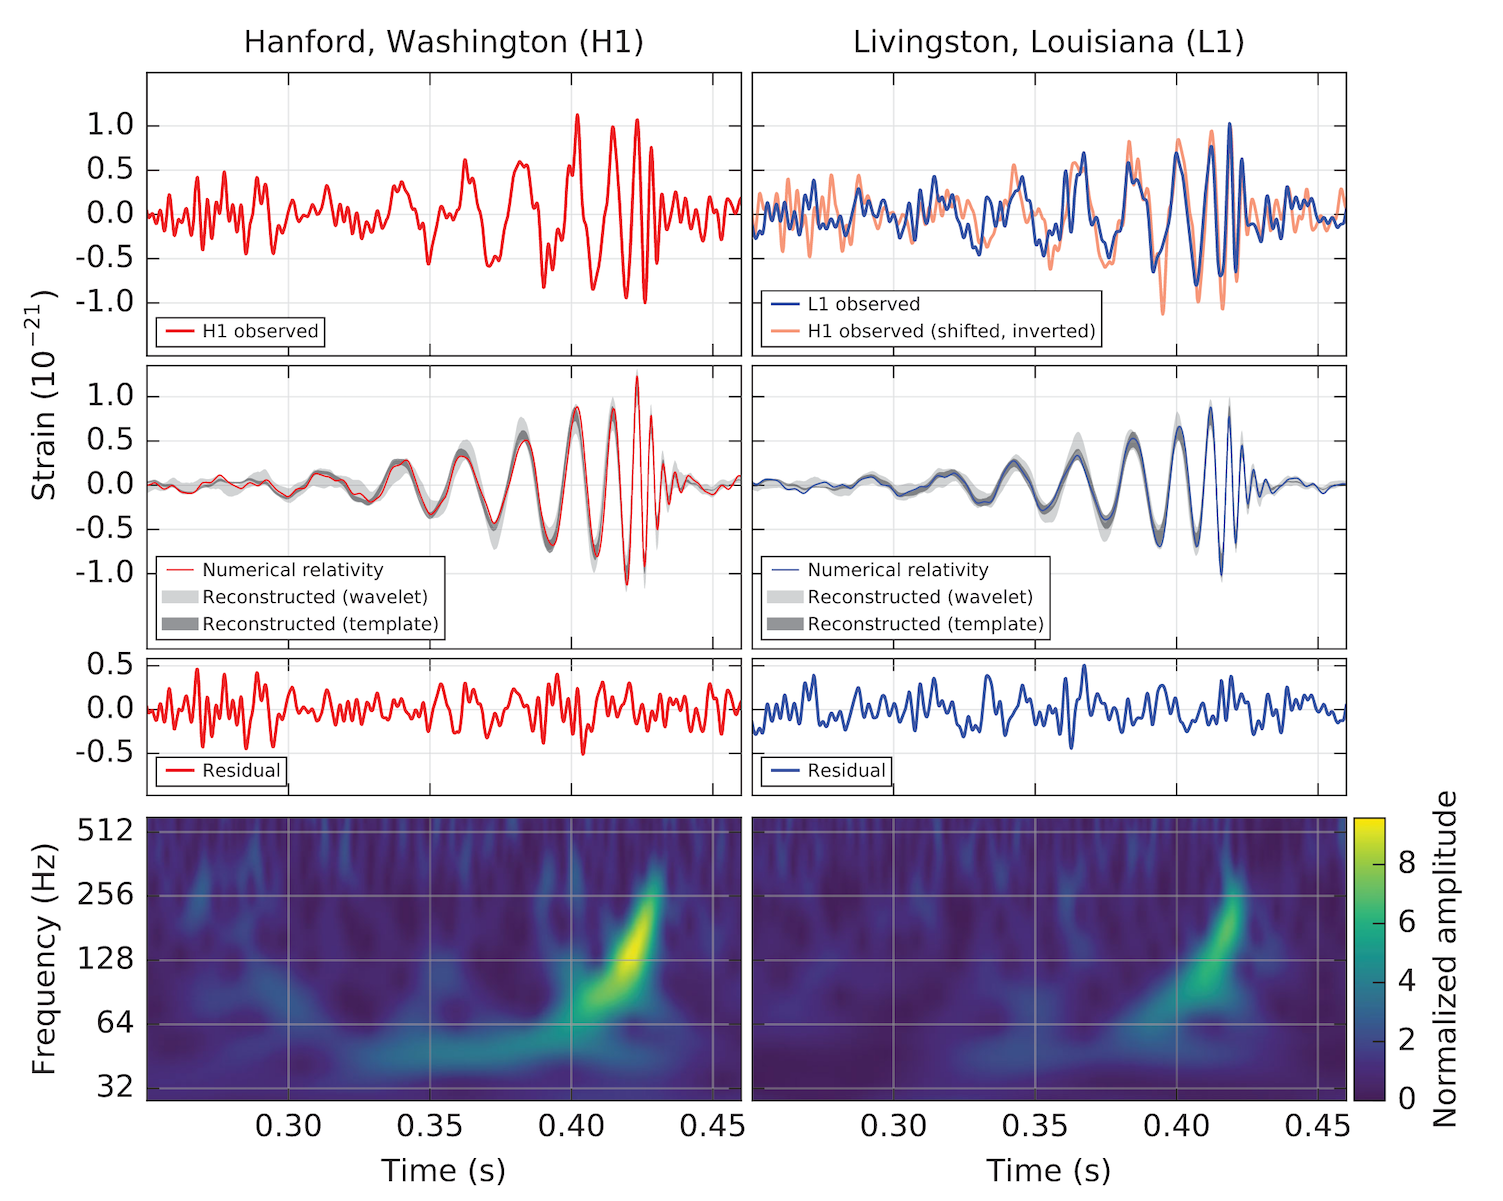
\includegraphics[width=\textwidth]{Assignments/figures/dc_fg.png}
  \end{center}
  \caption{The figure is from: B. P. Abbott et al. (LIGO Scientific Collaboration and Virgo Collaboration)
    Phys. Rev. Lett. 116, 061102 – Published 11 February 2016}
  \label{fig:ligo_result_plot}
\end{figure}


\section{7. Time delay}

Gravitational waves are expected to propagate at the speed of
light. The Hanford and Livingston detectors are separated by about
3000 km. A gravitational wave will propagate this distance in about 10 ms.

The gravitational wave angle of arrival is not known, but the relative
time delay between the signal detected at Hanford and Livingston is
expected to be $-10 < \tau < 10$ ms, if it is moving at the speed of
light in vacuum.
\begin{enumerate}[a)]

  \item Determine the time separation between the two signals \emph{by plotting the magnitudes}
        of the filtered gravitational wave signals ($|y_L[n]|$ and $|y_H[n+n_0]|$) with
        different delays $n_0$ on the same plot. Try different values of $n_0$ until the
        signals are approximately aligned in time. The magnitude of the signal is used to
        avoid phase-time ambiguities. Hint: Use magnitude, not amplitude.
        Magnitude can be obtained using \verb|numpy.abs|.

  \item What value do you obtain for the sample delay $n_0$?

  \item What time delay $\tau$ in seconds does the sample delay $n_0$ correspond to?

  \item Is the time delay $\tau$ in agreement with gravitational-wave
        propagation speed (i.e., that $-10 < \tau < 10$ ms)?

\end{enumerate}

\section{8. Dynamic spectrum}

\begin{marginfigure}
  \begin{center}
    \includegraphics[width=\textwidth]{Assignments/figures/dynspec.png}
  \end{center}
  \caption{A dynamic spectrum plot of the gravitational wave signal.}
  \label{fig:dynspec_ligo_ex}
\end{marginfigure}

Study the time-frequency behavior of the gravitational wave signal.
\begin{enumerate}[a)]

  \item Calculate the dynamic spectrum (spectrogram) of the low-pass
        filtered whitened signal $|\hat{x}[t,k]|$, where $t$ is time and $k$
        is frequency.

  \item Plot the dynamic power spectrum $|\hat{x}[t,k]|^2$ in dB scale.
        Perform this in such a way that you can see the time-frequency response
        behavior of the gravitational wave signal clearly. Plot your result at
        between $t=15.5$ s and $t=17$ s. Hint: You will need to use zero-padding,
        a tapered window, and overlapping windows. An example of the time-frequency
        domain behavior of the gravitational wave signal is shown in Figure \ref{fig:dynspec_ligo_ex}.


\end{enumerate}


\section{9. Extra task}
For earning an extra point, improve any part of the signal processing
in a way that you see fit. Document your improvements. You can, e.g.,
try to create a filter that removes only the strong frequency
components from the signal, or you can use a better low-pass filter.

\begin{figure}
  \begin{center}
    \includegraphics[width=\textwidth]{Assignments/figures/ligo_nobel.jpg}
  \end{center}
  \caption{The gravitational wave measurement using a Michelson-Morley interferometer. Credits: Johan Jarnestad, The Royal Swedish Academy of Sciences.}
  \label{fig:ligo_nobel_diag}
\end{figure}


\fi

\ifSpZFIR
\chapter{Z-transform}
\input{ch18/text18}
\input{ch18/exercises18}
 \ifSpExerciseSol
 \input{ch18/solutions18}
 \fi
\fi

\ifSpZIIR
\chapter{Infinite Impulse Response Filters}
\input{ch19/text19}
\input{ch19/exercises19}
 \ifSpExerciseSol
 \input{ch19/solutions19}
 \fi
\fi

\backmatter
\bibliography{bibliography} % Use the bibliography.bib file for the bibliography
\bibliographystyle{plainnat} % Use the plainnat style of referencing
\printindex

\end{document}
